% oneside + openany: sin páginas en blanco antes de cada capítulo (entrega en digital)
\documentclass[a4paper,11pt,oneside,openany]{book}
%\documentclass[a4paper,twoside,11pt,titlepage]{book}
\usepackage{listings}
\usepackage[utf8]{inputenc}
\usepackage[spanish,es-tabla]{babel}
\addto\captionsspanish{\renewcommand{\appendixname}{Anexo}}
\usepackage{float}
\raggedbottom
\usepackage{amsmath}
\usepackage{amssymb}
\usepackage{booktabs}
\usepackage{xspace}
\usepackage{xcolor}
\usepackage{adjustbox}
\usepackage{pgfgantt}          % diagrama de Gantt (Capítulo 4)
\usetikzlibrary{patterns,arrows.meta,positioning,fit,backgrounds,babel} % babel: evita conflictos de < > con el español
% Marca para contenido pendiente de completar (buscar "pendiente" en los .tex)
\newcommand{\pendiente}[1]{\textcolor{red}{\textbf{[PENDIENTE: #1]}}}
\usepackage{url}

% \usepackage[style=list, number=none]{glossary} %
%\usepackage{titlesec}
%\usepackage{pailatino}

\decimalpoint
\usepackage{dcolumn}
\newcolumntype{.}{D{.}{\esperiod}{-1}}
\makeatletter
\addto\shorthandsspanish{\let\esperiod\es@period@code}
\makeatother


%\usepackage[chapter]{algorithm}
\RequirePackage{verbatim}
%\RequirePackage[Glenn]{fncychap}
\usepackage{fancyhdr}
\usepackage{graphicx}
\usepackage{afterpage}

\usepackage{longtable}

\usepackage[pdfborder={0 0 0}]{hyperref} %referencia

% ********************************************************************
% Re-usable information
% ********************************************************************
\newcommand{\myTitle}{Compresión de agentes de Aprendizaje por Refuerzo Profundo para la Ingeniería de Tráfico\xspace}
\newcommand{\myDegree}{Grado en Ingeniería en Tecnologías de Telecomunicación\xspace}
\newcommand{\myName}{Marino Ramírez Pulido\xspace}
\newcommand{\myProf}{José Camacho Páez\xspace}
%\newcommand{\mySupervisor}{Put name here\xspace}
\newcommand{\myFaculty}{Escuela Técnica Superior de Ingenierías Informática y de
Telecomunicación\xspace}
\newcommand{\myFacultyShort}{E.T.S. de Ingenierías Informática y de
Telecomunicación\xspace}
\newcommand{\myDepartment}{Departamento de Teoría de la Señal, Telemática y Comunicaciones\xspace}
\newcommand{\myUni}{\protect{Universidad de Granada}\xspace}
\newcommand{\myLocation}{Granada\xspace}
\newcommand{\myTime}{\today\xspace}


\hypersetup{
	pdfauthor = {\myName},
	pdftitle = {\myTitle},
	pdfsubject = {},
	pdfkeywords = {redes autónomas, ingeniería de tráfico, aprendizaje por refuerzo profundo, redes neuronales de grafos, compresión de redes neuronales, poda, cuantización, destilación de conocimiento, programación lineal entera mixta, eficiencia energética},
	pdfcreator = {LaTeX},
	pdfproducer = {pdflatex}
}

%\hyphenation{}


%\usepackage{doxygen/doxygen}
%\usepackage{pdfpages}
\usepackage{url}
\usepackage{colortbl,longtable}
\usepackage[stable]{footmisc}
%\usepackage{index}

%\makeindex
%\usepackage[style=long, cols=2,border=plain,toc=true,number=none]{glossary}
% \makeglossary

% Definición de comandos que me son tiles:
%\renewcommand{\indexname}{Índice alfabético}
%\renewcommand{\glossaryname}{Glosario}

\pagestyle{fancy}
\fancyhf{}
% Cabeceras para impresión a una cara (oneside)
\fancyhead[L]{\leftmark}
\fancyhead[R]{\textbf{\thepage}}
\renewcommand{\chaptermark}[1]{\markboth{\textbf{#1}}{}}
\renewcommand{\sectionmark}[1]{\markright{\textbf{\thesection. #1}}}

\setlength{\headheight}{1.5\headheight}

\newcommand{\HRule}{\rule{\linewidth}{0.5mm}}
%Definimos los tipos teorema, ejemplo y definición podremos usar estos tipos
%simplemente poniendo \begin{teorema} \end{teorema} ...
\newtheorem{teorema}{Teorema}[chapter]
\newtheorem{ejemplo}{Ejemplo}[chapter]
\newtheorem{definicion}{Definición}[chapter]

\definecolor{gray97}{gray}{.97}
\definecolor{gray75}{gray}{.75}
\definecolor{gray45}{gray}{.45}
\definecolor{gray30}{gray}{.94}

\lstset{ frame=Ltb,
     framerule=0.5pt,
     aboveskip=0.5cm,
     framextopmargin=3pt,
     framexbottommargin=3pt,
     framexleftmargin=0.1cm,
     framesep=0pt,
     rulesep=.4pt,
     backgroundcolor=\color{gray97},
     rulesepcolor=\color{black},
     %
     stringstyle=\ttfamily,
     showstringspaces = false,
     basicstyle=\scriptsize\ttfamily,
     commentstyle=\color{gray45},
     keywordstyle=\bfseries,
     %
     numbers=left,
     numbersep=6pt,
     numberstyle=\tiny,
     numberfirstline = false,
     breaklines=true,
   }
 
% minimizar fragmentado de listados
\lstnewenvironment{listing}[1][]
   {\lstset{#1}\pagebreak[0]}{\pagebreak[0]}

\lstdefinestyle{CodigoC}
   {
	basicstyle=\scriptsize,
	frame=single,
	language=C,
	numbers=left
   }
\lstdefinestyle{CodigoC++}
   {
	basicstyle=\small,
	frame=single,
	backgroundcolor=\color{gray30},
	language=C++,
	numbers=left
   }

% Listados de Python (Capítulo 6). Los comentarios del código van sin tildes.
\lstdefinestyle{Python}
   {
	language=Python,
	basicstyle=\scriptsize\ttfamily,
	keywordstyle=\bfseries,
	commentstyle=\color{gray45}\itshape,
	frame=single,
	backgroundcolor=\color{gray97},
	numbers=left,
	numberstyle=\tiny,
	xleftmargin=1.5em,
	columns=fullflexible,
	keepspaces=true,
	showstringspaces=false
   }
\renewcommand{\lstlistingname}{Código}
\renewcommand{\lstlistlistingname}{Índice de códigos}

\lstdefinestyle{Consola}
   {basicstyle=\scriptsize\bf\ttfamily,
    backgroundcolor=\color{gray30},
    frame=single,
    numbers=none
   }


\newcommand{\bigrule}{\titlerule[0.5mm]}


%Para conseguir que en las páginas en blanco no ponga cabecerass
\makeatletter
\def\clearpage{%
  \ifvmode
    \ifnum \@dbltopnum =\m@ne
      \ifdim \pagetotal <\topskip
        \hbox{}
      \fi
    \fi
  \fi
  \newpage
  \thispagestyle{empty}
  \write\m@ne{}
  \vbox{}
  \penalty -\@Mi
}
\makeatother

\usepackage{pdfpages}
\begin{document}
\begin{titlepage}
 
 
\newlength{\centeroffset}
\setlength{\centeroffset}{-0.5\oddsidemargin}
\addtolength{\centeroffset}{0.5\evensidemargin}
\thispagestyle{empty}

\noindent\hspace*{\centeroffset}\begin{minipage}{\textwidth}

\centering

\includegraphics[width=0.9\textwidth]{imagenes/logo_ugr.jpg}\\[1.4cm]

\textsc{ \Large TRABAJO FIN DE GRADO\\[0.2cm]}
\textsc{ INGENIERÍA EN TECNOLOGÍAS DE TELECOMUNICACIÓN}\\[1cm]
% Upper part of the page
% 
% Title
{\Huge\bfseries Compresión de agentes de Aprendizaje por Refuerzo Profundo para la Ingeniería de Tráfico\\}
\noindent\rule[-1ex]{\textwidth}{3pt}\\[3.5ex]
{\large\bfseries Poda, Cuantización y Destilación del optimizador ENERO}
\end{minipage}

\vspace{0.8cm}
\noindent\hspace*{\centeroffset}
\begin{minipage}{\textwidth}
\centering
\textbf{Autor}\\ {Marino Ramírez Pulido}\\[2.5ex]
\textbf{Director}\\
{José Camacho Páez}\\[0.8cm]

\includegraphics[width=0.3\textwidth]{imagenes/etsiit_logo.png}\\[0.1cm]
\textsc{Escuela Técnica Superior de Ingenierías Informática y de Telecomunicación}\\
\textsc{---}\\
Granada, Noviembre de 2026
\end{minipage}
%\addtolength{\textwidth}{\centeroffset}
%\vspace{\stretch{2}}
\end{titlepage}



% =====================================================================
% prefacio.tex  (versión sin páginas en blanco innecesarias)
%  - Se elimina el \chapter*{} vacío del principio (generaba una página
%    sin contenido antes de la segunda portada).
%  - \cleardoublepage -> \clearpage (ya no se fuerza página impar).
%  - Las páginas de autorización e informe usan \clearpage en lugar de
%    \chapter*{} vacío.
% =====================================================================

% ---------------------------------------------------------------------
\clearpage
\thispagestyle{empty}

\noindent{\textbf{Palabras clave}: redes autónomas, ingeniería de tráfico, aprendizaje por refuerzo profundo, redes neuronales de grafos, compresión de redes neuronales, poda, cuantización, destilación de conocimiento, programación lineal entera mixta, eficiencia energética.}\\

\vspace{0.7cm}
\noindent{\textbf{Resumen}}\\

Las redes autónomas necesitan optimizar su configuración de forma continua, y el aprendizaje por refuerzo profundo (DRL) combinado con redes neuronales de grafos (GNN) se ha propuesto como alternativa rápida a los métodos clásicos de ingeniería de tráfico. ENERO es un ejemplo destacado: un agente DRL+GNN elige un nodo intermedio para cada demanda crítica y una búsqueda local refina después la solución. Sin embargo, la inferencia del agente se repite en cada ejecución del optimizador y su coste en memoria, tiempo y energía crece con el tamaño de la red. Este trabajo estudia si las técnicas de compresión de redes neuronales permiten reducir ese coste sin degradar la calidad del enrutamiento.

Para ello, se migró el entorno de simulación de ENERO a Gymnasium, se adaptó el entrenamiento a la ejecución en CPU y se entrenó un agente base. En el proceso se añadió a la recompensa un término de dispersión de la carga y se detectó, cuantificó y corrigió un sesgo sistemático en su primera implementación. Sobre el agente base se aplicaron la poda por magnitud con reentrenamiento, dos variantes de cuantización posterior al entrenamiento y la destilación de conocimiento hacia un estudiante 4,6 veces más pequeño, y todos los modelos se evaluaron en diez topologías no vistas, de 20 a 43 nodos, frente a OSPF, la búsqueda local, una cota de programación lineal y la formulación exacta del problema (MILP).

Los resultados muestran que la compresión conserva la calidad del enrutamiento: con la búsqueda local, los modelos comprimidos mejoran en media la utilización máxima de enlace de OSPF entre un 32,6 y un 35,0\,\% en las tres topologías principales, frente al 34,3\,\% del original, y rinden como él en siete redes mayores. La destilación es la técnica más adecuada para un procesador convencional: el estudiante acelera la inferencia 3,2 veces y reduce hasta un 25\,\% la energía por optimización, mientras que la poda y la cuantización solo reducen el tamaño del modelo. Sin embargo, al valorar también la aplicabilidad práctica, la metodología más adecuada para redes de este tamaño es la formulación exacta: resuelto sobre las mismas demandas críticas, el MILP supera a ENERO en las diez topologías, unas 70 veces más rápido y sin entrenamiento previo, y sobre todas las demandas alcanza prácticamente la cota de programación lineal. El agente, que requiere días de entrenamiento y generaliza mal, solo compensaría en redes mucho mayores, y comprimirlo no cambia esta conclusión.

% ---------------------------------------------------------------------
\clearpage
\thispagestyle{empty}

\noindent{\textbf{Keywords}: autonomous networks, traffic engineering, deep reinforcement learning, graph neural networks, neural network compression, pruning, quantization, knowledge distillation, mixed integer linear programming, energy efficiency.}\\

\vspace{0.7cm}
\noindent{\textbf{Abstract}}\\

Autonomous networks need to optimize their configuration continuously, and deep reinforcement learning (DRL) combined with graph neural networks (GNN) has been proposed as a fast alternative to classical traffic engineering methods. ENERO is a prominent example: a DRL+GNN agent selects a middlepoint for each critical demand, and a local search then refines the solution. However, the agent's inference is repeated every time the optimizer runs, and its memory, time and energy cost grows with the size of the network. This work studies whether neural network compression techniques can reduce that cost without degrading routing quality.

To this end, ENERO's simulation environment was migrated to Gymnasium, training was adapted to run on CPU, and a base agent was trained. In the process, a load-dispersion term was added to the reward, and a systematic bias in its first implementation was detected, quantified and corrected. Magnitude pruning with fine-tuning, two post-training quantization variants and knowledge distillation into a student 4.6 times smaller were applied to the base agent, and all models were evaluated on ten unseen topologies with 20 to 43 nodes, against OSPF, local search, a linear programming bound and the exact formulation of the problem (MILP).

The results show that compression preserves routing quality: combined with local search, the compressed models improve OSPF's maximum link utilization by 32.6 to 35.0\,\% on average on the three main topologies, compared with 34.3\,\% for the original, and perform like it on seven larger networks. Distillation is the most suitable technique for a general-purpose processor: the student speeds up inference by a factor of 3.2 and reduces energy per optimization by up to 25\,\%, whereas pruning and quantization only reduce model size. However, when practical applicability is also considered, the most suitable methodology for networks of this size is the exact formulation: solved over the same critical demands as the agent, the MILP outperforms ENERO on all ten topologies, about 70 times faster and without prior training, and over all demands it practically reaches the linear programming bound. The agent, which requires days of training and generalizes poorly, would only pay off on much larger networks, and compressing it does not change this conclusion.

% ---------------------------------------------------------------------
\frontmatter
\tableofcontents
\listoffigures
\listoftables
% \lstlistoflistings   % índice de códigos eliminado para cumplir el límite de 100 páginas
%
\mainmatter
\setlength{\parskip}{5pt}

\chapter{Introducción}\label{cap:int}

Las redes de telecomunicaciones se han convertido en una infraestructura crítica sobre la que se apoyan prácticamente todos los servicios digitales. El crecimiento sostenido del tráfico, la aparición de servicios con requisitos muy dispares y el despliegue de arquitecturas 5G y, en el futuro, 6G han multiplicado la complejidad de su operación. En este escenario, la configuración manual de la red resulta cada vez menos viable, y tanto la industria como los organismos de estandarización trabajan hacia el concepto de \textit{red autónoma}: una red capaz de monitorizarse, analizar su estado y tomar decisiones de reconfiguración con una intervención humana mínima \cite{coronado2022zero,etsi_zsm011}.

Este Trabajo Fin de Grado toca tres temas que suelen estudiarse por separado: la optimización del enrutamiento en redes de área extensa (WAN), el aprendizaje por refuerzo profundo (\textit{Deep Reinforcement Learning}, DRL) como forma de tomar esas decisiones de enrutamiento, y la compresión de redes neuronales para que un agente de DRL gaste menos memoria, tiempo y energía al ejecutarse.

\section{Contexto y motivación}\label{sec:int_motivacion}

En una red autónoma, la optimización deja de ser una tarea puntual realizada por un ingeniero para convertirse en una fase más de un bucle cerrado de control que se ejecuta de forma continua: se observa el estado de la red, se detecta una desviación respecto al objetivo del operador y se calcula y aplica una nueva configuración \cite{etsi_zsm016}. Uno de los problemas más representativos que se resuelven en ese bucle es la \textit{ingeniería de tráfico} (\textit{Traffic Engineering}, TE) intradominio: dado un conjunto de demandas de tráfico entre pares de nodos, decidir por qué caminos se cursa cada una para repartir la carga y evitar la congestión. Una métrica habitual para medir la calidad de una solución es la utilización máxima de enlace (\textit{Maximum Link Utilization}, MLU), es decir, la carga relativa del enlace más ocupado de la red.

El problema concreto que se aborda en este trabajo es el de \textbf{mínima congestión}: dadas una topología y una matriz de tráfico, encontrar el enrutamiento que minimiza la MLU, es decir, que reduce lo más posible la congestión del enlace más cargado. Si el tráfico de cada demanda pudiera dividirse libremente entre varios caminos, el problema sería lineal, y su solución óptima se obtendría de forma exacta mediante programación lineal (\textit{Linear Programming}, LP). En una red real, sin embargo, lo habitual es configurar un único camino por demanda, o a lo sumo unos pocos, y entonces el problema pasa a ser combinatorio. Para resolverlo se pueden utilizar métodos exactos de programación lineal entera mixta (\textit{Mixed Integer Linear Programming}, MILP), heurísticas como la búsqueda local o, más recientemente, aprendizaje por refuerzo. Este trabajo evalúa un método de este último tipo, ENERO, que combina un agente de aprendizaje por refuerzo profundo con una búsqueda local, y versiones comprimidas de su agente, y los compara con la solución exacta del problema.

Los protocolos de enrutamiento por el camino más corto, como OSPF, son sencillos y robustos, pero no tienen en cuenta la carga: todo el tráfico entre dos nodos sigue la misma ruta aunque esta atraviese enlaces saturados. Ajustar los pesos de OSPF para minimizar la congestión es un problema NP-hard \cite{fortz2000internet}, y los métodos exactos basados en programación entera escalan mal: su tiempo de resolución puede dispararse en redes grandes, lo que encaja mal en un bucle de control que tiene que reaccionar a los cambios del tráfico.

El DRL ofrece una alternativa: un agente aprende, mediante interacción con un entorno simulado, una política que propone buenas configuraciones en un tiempo muy reducido. Combinado con las redes neuronales de grafos (\textit{Graph Neural Networks}, GNN), capaces de procesar topologías de tamaño y forma arbitrarios, este enfoque ha dado lugar a optimizadores que generalizan a redes no vistas durante el entrenamiento. Un ejemplo destacado es ENERO \cite{ALMASAN2022109166}, que resuelve el problema de TE mediante enrutamiento por punto intermedio (\textit{middlepoint routing}): un agente DRL con una GNN elige, para cada demanda crítica, un nodo intermedio por el que forzar su paso y, a continuación, una búsqueda local (\textit{Local Search}, LS) refina la solución. ENERO constituye el caso de uso de este trabajo.

La ventaja temporal del DRL depende de que la inferencia del agente sea rápida, y esa inferencia tiene un coste. En ENERO, para cada demanda que se reubica, el actor evalúa la GNN sobre un grafo por cada nodo intermedio candidato, así que el número de pasadas por la red neuronal en una optimización crece con el número de nodos y con el de demandas críticas. Si el optimizador se ejecuta de forma continua dentro de un bucle de control, cada milisegundo y cada kilobyte se repiten miles de veces a lo largo de su vida útil. A ello se suma la preocupación creciente por el consumo energético de las tecnologías de la información y de los propios modelos de aprendizaje profundo, que ha dado lugar a la línea de trabajo conocida como \textit{Green Networking} \cite{bianzino2012survey,du2020green}, y la posibilidad de desplegar estos agentes en equipos con recursos limitados, más cerca de los elementos de red que controlan.

La compresión de redes neuronales, mediante técnicas como la poda de pesos, la cuantización o la destilación de conocimiento, persigue precisamente reducir el tamaño, la latencia y el consumo de los modelos manteniendo su calidad \cite{han2016deep,jacob2018quantization,hinton2015distilling}. Estas técnicas están muy maduras en aprendizaje supervisado, pero su aplicación a agentes de DRL está mucho menos estudiada \cite{ivanov2025neural}. En un agente de DRL hay una dificultad añadida: las decisiones son secuenciales y cada acción cambia el estado sobre el que se toman las siguientes, así que una pequeña desviación al principio puede alterar toda la trayectoria. En ENERO, reubicar una demanda cambia la carga de los enlaces y con ello las decisiones posteriores. No basta, por tanto, con medir cuánto se reduce el modelo; hay que comprobar si el agente comprimido sigue enrutando igual de bien.

Esta es la pregunta que motiva el trabajo: \textbf{¿es posible reducir de forma significativa el coste de ejecución de un agente DRL+GNN para ingeniería de tráfico sin degradar de manera apreciable la calidad del enrutamiento que produce?} Para valorar el alcance práctico de la respuesta, el trabajo plantea también una segunda pregunta: si un agente así, comprimido o no, compensa frente a resolver el mismo problema de forma exacta.

\section{Objetivos}\label{sec:int_objetivos}

El \textbf{objetivo general} de este trabajo es evaluar la aplicación de técnicas de compresión de redes neuronales al agente de DRL de ENERO, cuantificando el compromiso entre la reducción del coste computacional (memoria, latencia y energía) y la pérdida de calidad en la optimización del enrutamiento.

Para alcanzarlo se plantean los siguientes \textbf{objetivos específicos}:

\begin{enumerate}
	\item Estudiar la optimización en redes autónomas y las técnicas de compresión aplicables a agentes de DRL.
	\item Reproducir el agente de ENERO en un entorno software actual, adaptando su código a las bibliotecas vigentes, y entrenar un agente base que sirva de referencia.
	\item Analizar el diseño del entorno de simulación y de la función de recompensa, y corregir los problemas que puedan sesgar el aprendizaje o su interpretación.
	\item Aplicar al agente base tres familias de técnicas de compresión: poda de pesos con reentrenamiento, cuantización posterior al entrenamiento y destilación de conocimiento hacia un modelo estudiante de menor tamaño.
	\item Definir una metodología de evaluación que mida tanto el coste de los modelos (tamaño, número de parámetros y latencia de inferencia) como la calidad del enrutamiento (MLU, mejora frente a OSPF, distancia a una cota inferior obtenida por programación lineal y grado de coincidencia con las decisiones del modelo original).
	\item Comparar ENERO, con el modelo original y con los comprimidos, con la formulación exacta del mismo problema como programa lineal entero mixto (MILP), tanto en calidad del enrutamiento como en aplicabilidad práctica: tiempo de optimización, coste de entrenamiento y capacidad de generalizar a redes distintas.
	\item Estimar el impacto energético de cada alternativa y extraer conclusiones sobre la viabilidad de desplegar agentes comprimidos en redes autónomas y sobre la metodología más adecuada para este problema.
\end{enumerate}

\section{Contribuciones}\label{sec:int_contribuciones}

Las principales aportaciones de este trabajo son las siguientes:

\begin{itemize}
	\item La migración del entorno de simulación de ENERO (\textit{gym-graph}) de OpenAI Gym a Gymnasium y la adaptación del proceso de entrenamiento para que pueda ejecutarse de forma estable y más eficiente en un ordenador personal con GPU no compatible. 
	\item La incorporación a la recompensa de ENERO de un término de dispersión de la carga, que densifica la señal de aprendizaje, y la detección, explicación y corrección del sesgo que introducía su primera implementación, en una nueva versión del entorno. Con la recompensa corregida, el retorno de un episodio pasa a medir directamente la mejora respecto al enrutamiento inicial de OSPF, combinando la reducción de la MLU y la de la dispersión de la carga, y es positivo si y solo si esa combinación mejora. Esto facilita la interpretación del entrenamiento.
	\item La aplicación y comparación, sobre un mismo agente DRL+GNN, de poda por magnitud con reentrenamiento mediante PPO, de dos variantes de cuantización posterior al entrenamiento y de destilación de conocimiento hacia un estudiante con menos parámetros.
	\item Una metodología de evaluación centrada en la compresión, que separa el coste de la fase neuronal del coste de la optimización completa e incorpora métricas específicas, como la coincidencia de decisiones con el modelo original y la distancia a la cota de programación lineal.
	\item Una estimación del consumo energético asociado a cada variante, en línea con los objetivos de \textit{Green Networking}.
	\item Una comparación de ENERO, original y comprimido, con la formulación exacta del enrutamiento por punto intermedio, en dos variantes, que muestra que en redes de hasta 43 nodos el método exacto obtiene mejores soluciones, unas 70 veces más rápido y sin entrenamiento previo.
	\item Una evaluación adicional en siete topologías de 30 a 43 nodos, seis de ellas mayores que las utilizadas en el artículo original, para medir la generalización del agente original y de los comprimidos y su distancia a la cota de programación lineal a medida que crece la red.
\end{itemize}

\section{Alcance y limitaciones}\label{sec:int_alcance}

El trabajo se desarrolla íntegramente en simulación, sobre las topologías y matrices de tráfico del conjunto de datos publicado con ENERO, y no incluye un despliegue en equipos de red reales. La compresión se aplica únicamente al actor, que es la única red neuronal necesaria durante la inferencia; el crítico solo interviene en el entrenamiento. Todas las medidas de latencia se realizan en CPU de propósito general, por lo que no reflejan las aceleraciones que podría aportar hardware especializado, por ejemplo para explotar la dispersión de los modelos podados. Por último, el objetivo no es mejorar los resultados de ENERO, sino estudiar cuánto de su calidad se conserva al reducir el coste del agente y si, una vez comprimido, compensa frente a la formulación exacta del mismo problema. La comparación con otros optimizadores, como los que utiliza el artículo original, queda fuera del alcance.

\section{Uso de herramientas de inteligencia artificial generativa}\label{sec:int_ia}

Durante el desarrollo de este Trabajo Fin de Grado se ha utilizado una herramienta de inteligencia artificial generativa como apoyo en tareas de programación, análisis y redacción. Su uso se ha concentrado en los siguientes aspectos:

\begin{itemize}
	\item \textbf{Código}. Apoyo en errores en la adaptación del código de ENERO a las versiones actuales de las bibliotecas y en la localización de errores. Todas las figuras de resultados se han generado con estos scripts, en Python, a partir de los datos de los experimentos; no se han utilizado imágenes generadas por inteligencia artificial.
	\item \textbf{Análisis}. Revisión de cálculos y comprobación de que las cifras de la memoria coinciden con los ficheros de resultados.
	\item \textbf{Redacción}. Revisión de la estructura de la memoria, de la coherencia entre capítulos y de las referencias cruzadas.
\end{itemize}

El planteamiento del trabajo, el diseño de los experimentos, su ejecución y la interpretación de los resultados son del autor, y todos los resultados proceden de experimentos ejecutados por él. Cada propuesta de la herramienta se ha revisado antes de incorporarla, y se ha rechazado o modificado cuando no era correcta o no reflejaba el criterio del autor. Las cifras se han contrastado con los datos originales y el código se ha probado en el entorno del trabajo. Por tanto, el autor asume la plena responsabilidad del contenido de la memoria, de la corrección técnica del sistema implementado y de las conclusiones presentadas.

\section{Estructura de la memoria}\label{sec:int_estructura}

El resto del documento se organiza de la siguiente manera:

\begin{itemize}
	\item El \textbf{Capítulo~\ref{cap:opt}} presenta el marco de las redes autónomas, formaliza el problema de ingeniería de tráfico y revisa los métodos tradicionales para resolverlo y sus limitaciones. Introduce también los fundamentos del aprendizaje por refuerzo profundo, del algoritmo PPO y de las redes neuronales de grafos, y cómo se combinan en ENERO.
	\item El \textbf{Capítulo~\ref{cap:comp}} revisa las técnicas de compresión de redes neuronales (poda, cuantización y destilación de conocimiento), las particularidades de aplicarlas a agentes de DRL y su relación con la eficiencia energética.
	\item El \textbf{Capítulo~\ref{cap:plan}} recoge la planificación temporal del trabajo y la estimación de sus costes.
	\item El \textbf{Capítulo~\ref{cap:mat}} describe los materiales y métodos: el entorno software y hardware, ENERO, el entorno de simulación, el agente PPO, la cota de programación lineal, la formulación exacta MILP y las métricas de evaluación.
	\item El \textbf{Capítulo~\ref{cap:exp}} detalla el desarrollo experimental: la migración del entorno, la aceleración del entrenamiento, la corrección de la recompensa y la implementación del entrenamiento y de las tres técnicas de compresión.
	\item El \textbf{Capítulo~\ref{cap:pru}} presenta y analiza los resultados: el entrenamiento del agente base, el resultado de cada técnica de compresión, el coste de los modelos comprimidos, la calidad del enrutamiento que producen en topologías no vistas y en redes mayores, su impacto en el tiempo de optimización y en el consumo energético, su comparación con la formulación exacta del problema y qué metodología conviene según el tipo de red.
	\item El \textbf{Capítulo~\ref{cap:con}} expone las conclusiones y las líneas de trabajo futuro.
\end{itemize}

Finalmente, el Anexo~\ref{anx:topologias} muestra la estructura de las topologías de la evaluación principal.

%
\chapter{Optimización en redes autónomas}\label{cap:opt}

Este capítulo establece el marco teórico sobre el que se construye el trabajo. En primer lugar, se presenta el concepto de red autónoma y el papel que desempeña la optimización dentro de sus bucles de control (Sección~\ref{sec:redes_autonomas}). A continuación, se formaliza el problema de ingeniería de tráfico en redes WAN, que es el problema concreto que resuelve el caso de uso (Sección~\ref{sec:te}), y se revisan los métodos tradicionales para abordarlo junto con sus limitaciones (Sección~\ref{sec:metodos_trad}). Por último, se introducen los fundamentos del aprendizaje por refuerzo profundo (Sección~\ref{sec:drl}) y de las redes neuronales de grafos (Sección~\ref{sec:gnn}), y se describe cómo ambos se combinan para resolver problemas de ingeniería de tráfico (Sección~\ref{sec:drl_te}).

% =====================================================================
\section{Redes autónomas}\label{sec:redes_autonomas}

\subsection{Del paradigma manual a la autonomía}

Las redes 5G, y previsiblemente las 6G, conectan muchos más dispositivos que las generaciones anteriores, ofrecen servicios muy distintos entre sí y, en muchos casos, con requisitos de latencia estrictos. Operarlas a mano o con configuraciones estáticas deja de ser viable: hay demasiados parámetros que ajustar y cambian demasiado deprisa. Para abordar este desafío, la industria ha adoptado el paradigma de gestión de redes y servicios \textit{Zero-Touch} (\textit{Zero-Touch Network and Service Management}, ZSM), promovido por el ETSI.

La gestión \textit{Zero-Touch} se entiende como una gestión de red completamente autónoma, aunque sujeta a cierta supervisión humana. Su objetivo es minimizar la intervención de los operadores, evolucionando desde la simple automatización de tareas repetitivas hacia una autonomía completa en la que el sistema se gestiona a sí mismo para cumplir los objetivos de servicio \cite{coronado2022zero}.

\subsection{Intención y propiedades Self-X}

Es importante distinguir entre una red \textit{automatizada} y una red \textit{autónoma}. La automatización ejecuta tareas predefinidas conforme a reglas específicas; la autonomía, en cambio, implica la capacidad de decidir qué acciones tomar y ejecutarlas.

El pilar de esta autonomía es la gestión basada en intenciones (\textit{Intent-Driven Management}). El ETSI define una intención como la especificación de todas las expectativas, incluidos requisitos, objetivos y restricciones, que se proporcionan a un sistema técnico. A diferencia de la gestión tradicional, en la que se indica a la red \textit{cómo} ejecutar una tarea paso a paso, la intención es declarativa: especifica \textit{qué} resultado se desea y deja al sistema autónomo los detalles de su implementación. Esto da al sistema la flexibilidad necesaria para explorar distintas soluciones y elegir la más adecuada sin intervención humana directa \cite{etsi_zsm011}.

La autonomía se materializa a través de un conjunto de capacidades conocidas como propiedades \textit{Self-X}:

\begin{itemize}
	\item \textit{Self-configuration}: capacidad de desplegar, integrar y configurar automáticamente nuevos componentes o funciones de red, físicos o virtuales, en cuanto se conectan.
	\item \textit{Self-healing}: capacidad de detectar, diagnosticar y recuperarse de fallos o degradaciones del servicio, aislando el problema y ejecutando acciones correctivas.
	\item \textit{Self-protection}: capacidad de defender la infraestructura y los datos frente a ataques o accesos no autorizados, identificando patrones anómalos y mitigando amenazas.
	\item \textit{Self-optimization}: capacidad de monitorizar continuamente el rendimiento y ajustar dinámicamente la asignación de recursos (espectro, potencia, enrutamiento, etc.) para maximizar la eficiencia y cumplir los acuerdos de nivel de servicio (\textit{Service Level Agreements}, SLA) ante las fluctuaciones del tráfico.
\end{itemize}

Este trabajo se enmarca en la última de ellas: la optimización automática del enrutamiento ante cambios en la demanda de tráfico.

\subsection{Bucles cerrados y el ciclo MAPE-K}\label{sec:mapek}

Para hacer operativas estas propiedades y mantener la red alineada con las intenciones del operador, la arquitectura ZSM se apoya en bucles cerrados de control (\textit{closed loops}). Un bucle cerrado persigue un objetivo concreto monitorizando y regulando de forma continua un conjunto de entidades gestionadas: observa el estado de la red, analiza su discrepancia con la intención, decide las acciones correctivas y las ejecuta \cite{etsi_zsm016}.

El modelo de referencia que describe este comportamiento es el ciclo MAPE-K (\textit{Monitor, Analyze, Plan, Execute, Knowledge}), propuesto originalmente por IBM en el contexto de la computación autonómica \cite{kephart2003vision}. El ciclo descompone la autonomía en cuatro fases que operan sobre una base de conocimiento compartida:

\begin{itemize}
	\item \textbf{Monitorización}: recogida continua de métricas y telemetría para capturar el estado del sistema.
	\item \textbf{Análisis}: procesamiento de esos datos para detectar patrones, anomalías o desviaciones respecto a la intención.
	\item \textbf{Planificación}: selección de las acciones que corrigen el estado de la red. Es aquí donde reside la optimización: ya sea mediante algoritmos exactos, heurísticas o agentes de aprendizaje, el optimizador es el componente que decide qué hacer para cumplir el objetivo.
	\item \textbf{Ejecución}: aplicación de los cambios de configuración en la infraestructura física o virtual.
\end{itemize}

El componente de conocimiento almacena tanto el historial de la red como los modelos que guían las decisiones. En el paradigma de las redes definidas por conocimiento (\textit{Knowledge-Defined Networking}, KDN), este plano de conocimiento se apoya en técnicas de aprendizaje automático para que el sistema no solo reaccione, sino que aprenda de experiencias pasadas y mejore sus decisiones futuras \cite{mestres2017knowledge,he2023routing}. Los estándares ZSM reconocen explícitamente la inteligencia artificial como un habilitador de esta automatización y definen servicios de gestión para el entrenamiento, la inferencia y la validación de modelos dentro del ciclo de vida de la red \cite{etsi_zsm012}.

Desde el punto de vista de este trabajo, la consecuencia más relevante del modelo MAPE-K es que la optimización no es una tarea que se ejecute una vez, sino una fase que se repite cada vez que el bucle detecta un cambio. El coste de cada ejecución del optimizador, en tiempo y en energía, se multiplica por el número de veces que se ejecuta el bucle a lo largo de la vida de la red.

% =====================================================================
\section{Ingeniería de tráfico en redes WAN}\label{sec:te}

Una red autónoma debe resolver problemas de optimización de naturaleza muy diversa. Este trabajo se centra en uno de los más estudiados: la ingeniería de tráfico (\textit{Traffic Engineering}, TE) intradominio en redes de área extensa (WAN), es decir, la decisión de por qué caminos se cursa el tráfico dentro de la red de un operador para aprovechar sus recursos y evitar la congestión.

\subsection{Modelo de red y utilización máxima de enlace}\label{sec:mlu}

La red se modela como un grafo dirigido $G=(V,E)$, donde $V$ es el conjunto de nodos (enrutadores) y $E$ el conjunto de enlaces. Cada enlace físico bidireccional se representa mediante dos enlaces dirigidos, y cada enlace $e \in E$ tiene una capacidad $c_e > 0$. El tráfico se describe mediante una matriz de tráfico (\textit{Traffic Matrix}, TM), que puede verse como un conjunto de demandas $\mathcal{D}$, donde cada demanda $k \in \mathcal{D}$ se caracteriza por un nodo origen $s_k$, un nodo destino $d_k$ y un ancho de banda $b_k$. En una red de $|V|$ nodos puede haber hasta $|V|(|V|-1)$ demandas, un número que crece de forma cuadrática con el tamaño de la red.

Una configuración de enrutamiento asigna a cada demanda uno o varios caminos. Si $x_{k,e} \in [0,1]$ denota la fracción del tráfico de la demanda $k$ que atraviesa el enlace $e$, la carga y la utilización del enlace son:
\begin{equation}
	L_e = \sum_{k \in \mathcal{D}} x_{k,e}\, b_k, \qquad u_e = \frac{L_e}{c_e}.
\end{equation}

Un enlace está congestionado cuando $u_e > 1$, es decir, cuando la carga que recibe supera su capacidad y el exceso de paquetes se descarta. El objetivo clásico de la TE, y el que se adopta en este trabajo siguiendo a \cite{ALMASAN2022109166}, es minimizar la utilización máxima de enlace (\textit{Maximum Link Utilization}, MLU):
\begin{equation}\label{eq:mlu}
	\mathrm{MLU} = \max_{e \in E} u_e .
\end{equation}

La MLU es adimensional, porque es un cociente entre carga y capacidad. En una red bien dimensionada suele mantenerse por debajo de 0,5--0,6, para dejar margen ante picos de tráfico; un valor superior a 1 indica que el enlace más cargado recibe más tráfico del que puede cursar.

Minimizar la MLU equivale a alejar el enlace más cargado de la saturación, lo que reduce el riesgo de congestión y de pérdidas. Es una métrica sencilla e interpretable, aunque solo depende del peor enlace: dos configuraciones con la misma MLU pueden repartir la carga de forma muy distinta en el resto de la red. Por este motivo, es habitual acompañarla de alguna medida de la dispersión de las utilizaciones, como su desviación típica.

\subsection{Enrutamiento por el camino más corto: OSPF}\label{sec:ospf}

En las redes IP, el enrutamiento intradominio suele realizarse con protocolos de estado de enlace como OSPF (\textit{Open Shortest Path First}). Cada enlace tiene asignado un peso y cada enrutador calcula, mediante el algoritmo de Dijkstra, el camino de menor coste hacia cada destino. Cuando existen varios caminos con el mismo coste, el tráfico puede repartirse entre ellos (\textit{Equal-Cost Multi-Path}, ECMP).

OSPF es sencillo, distribuido y robusto, pero no tiene en cuenta la carga: todo el tráfico hacia un destino sigue el mismo camino aunque atraviese enlaces saturados mientras otros permanecen infrautilizados. La única forma de influir en el reparto es modificar los pesos de los enlaces. Sin embargo, encontrar el conjunto de pesos que minimiza la congestión para una matriz de tráfico dada es un problema NP-hard, y los pesos óptimos para una matriz pueden ser malos para otra \cite{fortz2000internet}. Además, cambiar un peso modifica simultáneamente el camino de todas las demandas que atraviesan ese enlace, lo que dificulta un control fino. En este trabajo, OSPF se utiliza como configuración de partida y como referencia mínima que cualquier optimizador debe mejorar.

\subsection{Segment Routing y enrutamiento por punto intermedio}\label{sec:sr}

El enrutamiento por segmentos (\textit{Segment Routing}, SR) permite un control mucho más fino sin sustituir el enrutamiento por el camino más corto \cite{rfc8402}. En SR, el nodo de entrada incluye en la cabecera de cada paquete una lista de segmentos que debe recorrer; dentro de cada segmento, el paquete se encamina por el camino más corto habitual. De esta forma, un controlador centralizado puede desviar una demanda concreta por un nodo determinado sin modificar los pesos de la red ni el camino del resto de demandas.

Un caso particular especialmente útil es el enrutamiento por punto intermedio (\textit{middlepoint routing}), en el que cada demanda se desvía como máximo por un nodo intermedio $m \in V$. El camino resultante es la concatenación del camino más corto de $s_k$ a $m$ y del camino más corto de $m$ a $d_k$:
\begin{equation}
	P_k(m) = \mathrm{SP}(s_k, m) \oplus \mathrm{SP}(m, d_k),
\end{equation}
donde elegir $m = s_k$ o $m = d_k$ equivale a mantener el camino de OSPF. Se ha demostrado que las rutas de dos segmentos ofrecen flexibilidad suficiente para alcanzar un rendimiento cercano al óptimo en muchas redes \cite{bhatia2015optimized}.

Este planteamiento convierte la TE en un problema combinatorio: para cada demanda hay $|V|$ opciones y el número total de configuraciones posibles es del orden de $|V|^{|\mathcal{D}|}$. Además, las decisiones no son independientes, porque desviar una demanda cambia la carga de los enlaces y, con ello, la conveniencia de desviar las demás. Este es el problema que resuelve ENERO \cite{ALMASAN2022109166}, el caso de uso de este trabajo, descrito en detalle en la Sección~\ref{sec:enero}.

% =====================================================================
\section{Métodos tradicionales de optimización y sus limitaciones}\label{sec:metodos_trad}

Antes de la irrupción del aprendizaje profundo, la optimización de redes se basaba en técnicas matemáticas y algorítmicas que no requieren entrenamiento, sino que operan con reglas explícitas o modelos definidos por expertos. Para el problema de mínima congestión de la Sección~\ref{sec:mlu}, lo que más condiciona el método es si se admite que el tráfico de una demanda se divida entre varios caminos, caso en el que la programación lineal da la solución óptima, o si, como en una red real, cada demanda sigue un único camino o unos pocos. Para este segundo caso hay métodos exactos (Sección~\ref{sec:prog_mat}), heurísticos (Sección~\ref{sec:heuristicas}) y, más recientemente, basados en aprendizaje por refuerzo (Sección~\ref{sec:drl_te}).

\subsection{Programación matemática}\label{sec:prog_mat}

La aproximación más rigurosa consiste en formular el problema como un programa matemático, con una función objetivo y un conjunto de restricciones sobre variables de decisión \cite{zhu2021network}. Conviene distinguir dos casos, porque su coste es muy diferente:

\begin{itemize}
	\item Si se permite que el tráfico de cada demanda se reparta de forma arbitraria entre varios caminos, minimizar la MLU es un problema de flujo multicomodidad (\textit{Multi-Commodity Flow}, MCF) que puede formularse como un programa lineal (\textit{Linear Programming}, LP) con variables continuas. Un LP se resuelve en tiempo polinómico, aunque el número de variables crece con el producto del número de demandas y de enlaces, por lo que en redes grandes su resolución puede requerir segundos o más. Existen formulaciones alternativas que reducen ese número, agregando las demandas por destino o limitando cada demanda a un conjunto de caminos predefinidos.
	\item Si el enrutamiento está restringido a mecanismos realistas, como un único camino por demanda, los pesos de OSPF o el enrutamiento por punto intermedio, aparecen variables enteras y el problema pasa a ser de programación lineal entera (\textit{Integer Linear Programming}, ILP) o normalmente programación lineal entera mixta (\textit{Mixed Integer Linear Programming}, MILP), en general NP-hard. Su tiempo de resolución puede crecer de forma exponencial con el tamaño de la red, aunque los \textit{solvers} actuales resuelven en poco tiempo muchas instancias de tamaño moderado, como se comprueba en la Sección~\ref{sec:res_milp}.
\end{itemize}

La solución del LP de flujo multicomodidad tiene una propiedad muy útil: como es la relajación de cualquier esquema de enrutamiento más restrictivo, su MLU es una \textbf{cota inferior} de la MLU alcanzable con OSPF, con enrutamiento por punto intermedio o con cualquier otro esquema. Por eso se utiliza en este trabajo como referencia de lo que sería posible en el mejor caso (Sección~\ref{sec:lp}), aunque no sea directamente desplegable.

\subsection{Heurísticas y metaheurísticas}\label{sec:heuristicas}

Para superar las limitaciones de escalabilidad de los métodos exactos, la ingeniería de redes ha recurrido históricamente a heurísticas: algoritmos diseñados por expertos que renuncian a garantizar el óptimo a cambio de encontrar una solución suficientemente buena en un tiempo razonable, a menudo reduciendo el espacio de búsqueda con reglas específicas del problema \cite{meng2020topology}. El propio problema de ajuste de pesos de OSPF se abordó con una heurística de LS \cite{fortz2000internet}.

Las metaheurísticas, como la LS, el recocido simulado, la búsqueda tabú o los algoritmos genéticos, exploran el espacio de soluciones sin depender tanto de la estructura del problema \cite{bello2016neural}. En el ámbito de la TE con \textit{Segment Routing} destaca DEFO \cite{hartert2015declarative}, que utiliza programación con restricciones para encontrar configuraciones de alta calidad. Estos métodos son más flexibles que los exactos, pero su tiempo de ejecución crece rápidamente con el tamaño de la red, requieren un ajuste manual considerable y pueden estancarse en óptimos locales.

\subsection{Limitaciones en redes dinámicas}\label{sec:limitaciones}

Los métodos anteriores han sido la base de la gestión de redes durante décadas, pero presentan tres limitaciones importantes cuando la optimización debe ejecutarse dentro de un bucle cerrado:

\begin{itemize}
	\item \textbf{Dependencia de modelos explícitos}. La programación matemática y la teoría de control necesitan un modelo analítico del sistema, que a menudo recurre a simplificaciones. Cuando el modelo se aleja de la realidad (interferencias, movilidad, ráfagas de tráfico), la calidad de la solución se degrada \cite{yang2022comparative}.
	\item \textbf{Coste computacional}. Los métodos exactos con variables enteras y las metaheurísticas escalan mal con el tamaño de la red (Sección~\ref{sec:prog_mat}). En redes grandes, el tiempo que requieren puede ser incompatible con la frecuencia a la que cambia el tráfico \cite{li2023topology}.
	\item \textbf{Falta de aprendizaje}. Cada nueva matriz de tráfico se resuelve desde cero, sin aprovechar la experiencia acumulada en situaciones anteriores. Los protocolos como OSPF, por su parte, reaccionan con información local y sin capacidad de anticipación \cite{he2023routing,xiao2023cognitive}. En un bucle que debe reaccionar en tiempo real, se requieren métodos capaces de optimizar de forma continua sin recalcular todo ante cada cambio \cite{abo2024toward}.
\end{itemize}

Estas limitaciones motivan el uso de métodos basados en aprendizaje, y en particular del aprendizaje por refuerzo: un agente puede aprender, mediante interacción con un entorno, una política que proponga buenas configuraciones en un tiempo muy reducido, sin necesidad de un modelo explícito del sistema. El coste se traslada así de la fase de decisión a una fase de entrenamiento previa, que solo se realiza una vez.

% =====================================================================
\section{Aprendizaje por refuerzo profundo}\label{sec:drl}

El aprendizaje por refuerzo (\textit{Reinforcement Learning}, RL) es la rama del aprendizaje automático que estudia cómo un agente aprende a tomar decisiones secuenciales mediante la interacción con un entorno, guiado por una señal de recompensa \cite{sutton2018reinforcement}. A diferencia del aprendizaje supervisado, no necesita ejemplos etiquetados con la decisión correcta, que en la operación de redes serían muy costosos de obtener: le basta con poder evaluar las consecuencias de sus acciones.

\subsection{Procesos de decisión de Markov}

El problema se formaliza como un proceso de decisión de Markov (\textit{Markov Decision Process}, MDP), definido por la tupla $(\mathcal{S}, \mathcal{A}, P, R, \gamma)$: un conjunto de estados $\mathcal{S}$, un conjunto de acciones $\mathcal{A}$, una función de transición $P(s' \mid s, a)$, una función de recompensa $R(s,a)$ y un factor de descuento $\gamma \in [0,1)$. En cada instante $t$, el agente observa el estado $s_t$, elige una acción $a_t$ según su política $\pi(a \mid s)$, recibe una recompensa $r_t$ y el entorno pasa a un nuevo estado $s_{t+1}$. El objetivo es encontrar la política que maximiza el retorno esperado:
\begin{equation}\label{eq:retorno}
	G_t = \sum_{i=0}^{\infty} \gamma^{i}\, r_{t+i}, \qquad \pi^{*} = \arg\max_{\pi}\, \mathbb{E}_{\pi}\left[ G_0 \right].
\end{equation}

Para valorar estados y acciones se definen la función de valor $V^{\pi}(s) = \mathbb{E}_{\pi}[G_t \mid s_t = s]$, que mide el retorno esperado desde un estado, y la función de valor de acción $Q^{\pi}(s,a) = \mathbb{E}_{\pi}[G_t \mid s_t = s, a_t = a]$. Su diferencia, la \textit{ventaja} $A^{\pi}(s,a) = Q^{\pi}(s,a) - V^{\pi}(s)$, indica cuánto mejor es una acción que el comportamiento medio de la política en ese estado.

Los métodos que se estudian en este trabajo son \textit{model-free}: el agente no conoce ni intenta aprender $P$, sino que aprende directamente la política o las funciones de valor a partir de las transiciones que observa. En el caso de la TE, esto significa que el agente no necesita un modelo analítico de la red, solo un entorno (real o simulado) que le devuelva el nuevo estado de carga y la recompensa tras cada decisión.

\subsection{Del aprendizaje por refuerzo al DRL}\label{sec:actor_critico}

Cuando el espacio de estados es grande o continuo, como ocurre con el estado de carga de una red, no es posible representar la política o las funciones de valor mediante tablas. El aprendizaje por refuerzo profundo (\textit{Deep Reinforcement Learning}, DRL) utiliza redes neuronales profundas como aproximadores de estas funciones. Su éxito en tareas de gran complejidad, como el control de videojuegos a partir de píxeles \cite{mnih2015human}, impulsó su aplicación a numerosos problemas de ingeniería, entre ellos la optimización de redes \cite{he2023routing,abo2024toward}.

Existen dos grandes familias de métodos. Los métodos basados en valor, como DQN \cite{mnih2015human}, aprenden $Q(s,a)$ y eligen la acción de mayor valor. Los métodos de gradiente de política, en cambio, parametrizan directamente la política $\pi_\theta$ mediante una red neuronal de parámetros $\theta$ y la mejoran siguiendo el gradiente del retorno esperado:
\begin{equation}\label{eq:policy_gradient}
	\nabla_\theta J(\theta) = \mathbb{E}_{\pi_\theta}\left[ \nabla_\theta \log \pi_\theta(a_t \mid s_t)\, \hat{A}_t \right],
\end{equation}
donde $\hat{A}_t$ es una estimación de la ventaja. Los métodos \textbf{actor-crítico} combinan ambas ideas mediante dos redes: el \textit{actor}, que implementa la política $\pi_\theta$ y decide las acciones, y el \textit{crítico}, que estima la función de valor $V_\phi(s)$ y se utiliza para calcular $\hat{A}_t$, reduciendo la varianza del gradiente.

Esta separación tiene una consecuencia importante para este trabajo: el crítico solo se necesita durante el entrenamiento. Una vez desplegado, el agente toma decisiones utilizando únicamente el actor, por lo que es el actor el que determina el coste de inferencia y el que tiene sentido comprimir.

\subsection{Proximal Policy Optimization}\label{sec:ppo}

\textit{Proximal Policy Optimization} (PPO) \cite{schulman2017proximal} es uno de los algoritmos actor-crítico más utilizados por su estabilidad y sencillez, y es el que emplea ENERO. Los métodos de gradiente de política son sensibles al tamaño de cada actualización: un paso demasiado grande puede alejar la política de la región en la que se recogieron los datos y degradarla de forma irreversible. PPO limita este efecto mediante un objetivo recortado. Sea
\begin{equation}
	\rho_t(\theta) = \frac{\pi_\theta(a_t \mid s_t)}{\pi_{\theta_{\text{old}}}(a_t \mid s_t)}
\end{equation}
el cociente entre la probabilidad de la acción con la política actual y con la política que recogió los datos. PPO maximiza:
\begin{equation}\label{eq:ppo_clip}
	L^{\text{CLIP}}(\theta) = \mathbb{E}_t\left[ \min\left( \rho_t(\theta)\,\hat{A}_t,\ \operatorname{clip}\left(\rho_t(\theta), 1-\epsilon, 1+\epsilon\right)\hat{A}_t \right) \right],
\end{equation}
donde $\epsilon$ (típicamente 0,1--0,2) acota cuánto puede cambiar la probabilidad de cada acción en una actualización. Gracias a ello, los mismos datos pueden reutilizarse durante varias épocas de optimización con minilotes.

La función de pérdida completa combina el objetivo del actor, el error cuadrático del crítico y un término de entropía que favorece la exploración:
\begin{equation}\label{eq:ppo_loss}
	L(\theta, \phi) = -L^{\text{CLIP}}(\theta) + c_1\, \mathbb{E}_t\left[ \left(V_\phi(s_t) - \hat{G}_t\right)^2 \right] - c_2\, \mathbb{E}_t\left[ \mathcal{H}\left(\pi_\theta(\cdot \mid s_t)\right) \right],
\end{equation}
donde $\hat{G}_t$ es el retorno estimado, $\mathcal{H}$ es la entropía de la distribución de acciones y $c_1$, $c_2$ son coeficientes de ponderación.

La ventaja se estima habitualmente con el estimador GAE (\textit{Generalized Advantage Estimation}) \cite{schulman2016high}, que combina diferencias temporales de distintos horizontes:
\begin{equation}\label{eq:gae}
	\delta_t = r_t + \gamma V_\phi(s_{t+1}) - V_\phi(s_t), \qquad \hat{A}_t = \sum_{i=0}^{\infty} (\gamma\lambda)^{i}\, \delta_{t+i},
\end{equation}
donde $\lambda \in [0,1]$ regula el compromiso entre sesgo y varianza. Los valores concretos de estos hiperparámetros en el entrenamiento del agente base se detallan en la Sección~\ref{sec:hiperparametros_base}.

% =====================================================================
\section{Redes neuronales de grafos}\label{sec:gnn}

Las redes neuronales convencionales, como los perceptrones multicapa o las redes convolucionales, esperan entradas de tamaño y estructura fijos. Una red de comunicaciones, en cambio, es un grafo cuyo número de nodos y enlaces varía de una topología a otra. Las redes neuronales de grafos (\textit{Graph Neural Networks}, GNN) \cite{scarselli2009graph} están diseñadas para procesar directamente este tipo de datos.

\subsection{Paso de mensajes}\label{sec:mpnn}

La formulación más extendida es la de paso de mensajes (\textit{Message Passing Neural Network}, MPNN) \cite{gilmer2017neural}. Cada elemento del grafo $v$ tiene asociado un estado oculto $h_v$, inicializado a partir de sus características. Durante $T$ iteraciones, cada elemento recibe mensajes de sus vecinos $\mathcal{N}(v)$ y actualiza su estado:
\begin{align}
	m_v^{(t+1)} &= \sum_{w \in \mathcal{N}(v)} M\left(h_v^{(t)}, h_w^{(t)}\right), \label{eq:mp_msg}\\
	h_v^{(t+1)} &= U\left(h_v^{(t)}, m_v^{(t+1)}\right), \label{eq:mp_upd}
\end{align}
donde $M$ es la función de mensaje y $U$ la función de actualización, ambas implementadas con redes neuronales (por ejemplo, una capa densa y una celda recurrente GRU). Tras las $T$ iteraciones, una función de lectura (\textit{readout}) $R$ agrega los estados de todos los elementos y produce la salida:
\begin{equation}\label{eq:readout}
	y = R\left(\left\{ h_v^{(T)} \mid v \in G \right\}\right).
\end{equation}

Esta formulación tiene dos propiedades clave. Las funciones $M$, $U$ y $R$ son las mismas para todos los elementos, por lo que el número de parámetros no depende del tamaño del grafo y un mismo modelo puede aplicarse a topologías distintas. Además, al agregar mediante sumas, el resultado no depende del orden en que se numeren los elementos. Como contrapartida, el coste de inferencia sí crece con el tamaño del grafo y con el número de iteraciones $T$: cada iteración aplica $M$ y $U$ a todos los elementos.

\subsection{GNN en redes de comunicaciones}

Las GNN se han consolidado como la herramienta de referencia para modelar redes de comunicaciones. RouteNet \cite{rusek2020routenet}, por ejemplo, utiliza paso de mensajes entre enlaces y caminos para estimar el retardo y las pérdidas de una configuración, y generaliza a topologías no vistas durante el entrenamiento. En los problemas de enrutamiento es habitual asociar los estados ocultos a los \textit{enlaces}, cuyas características (capacidad, utilización) son las que determinan la congestión, e intercambiar mensajes entre enlaces vecinos. Esta es la representación que utiliza el agente de ENERO, descrito en la Sección~\ref{sec:agente}.

% =====================================================================
\section{Aprendizaje por refuerzo aplicado a la ingeniería de tráfico}\label{sec:drl_te}

La naturaleza secuencial de muchas decisiones de red, en las que cada acción modifica el estado sobre el que se toman las siguientes, encaja de forma natural con el DRL. Se han propuesto agentes de DRL para el enrutamiento en redes definidas por conocimiento \cite{he2023routing} y para el enrutamiento cognitivo en redes autónomas \cite{xiao2023cognitive}, entre otros. Sin embargo, los agentes basados en redes neuronales convencionales tienen dificultades para generalizar a topologías distintas de las de entrenamiento, ya que su entrada tiene un tamaño fijo ligado a una red concreta.

La combinación de DRL y GNN resuelve esta limitación. ENERO \cite{ALMASAN2022109166} aborda el problema de TE con enrutamiento por punto intermedio (Sección~\ref{sec:sr}) en dos etapas. En la primera, un agente DRL entrenado con PPO recorre las demandas críticas, que son una fracción de las demandas que atraviesan los enlaces más cargados, y asigna a cada una un nodo intermedio. Para elegirlo, el actor evalúa la GNN sobre una copia del grafo por cada nodo intermedio candidato, en la que se marcan los enlaces del camino resultante, y obtiene una distribución de probabilidad sobre las acciones. En la segunda etapa, una LS refina la solución. El agente parte siempre de la configuración de OSPF y, si no consigue mejorarla, se conserva la configuración inicial, lo que garantiza que el resultado nunca es peor que el de partida.

Este diseño tiene una implicación directa sobre el coste de inferencia. Si una optimización reubica $D_c$ demandas críticas en una red de $|V|$ nodos, el actor realiza del orden de $D_c \cdot |V|$ pasadas por la GNN, cada una con $T$ iteraciones de paso de mensajes sobre todos los enlaces del grafo. El tiempo de la fase neuronal crece, por tanto, con el tamaño de la red y con el tamaño del propio modelo, y se repite en cada ejecución del bucle de control (Sección~\ref{sec:mapek}). Reducir el coste de cada pasada mediante la compresión del actor, sin degradar la calidad de sus decisiones, es el objetivo del resto de este trabajo. Las técnicas disponibles para ello se revisan en el Capítulo~\ref{cap:comp}.

%
\chapter{Compresión en Deep Reinforcement Learning}\label{cap:comp}

Las redes neuronales profundas permiten a los agentes de DRL aprender políticas de control sofisticadas, pero su ejecución tiene un coste en memoria, tiempo de cálculo y energía. En el caso de un optimizador de red como ENERO, ese coste se paga en cada ejecución del bucle de control y crece con el tamaño de la red (Sección~\ref{sec:drl_te}). Además, la posibilidad de ejecutar estos agentes en equipos con recursos limitados, más cerca de los elementos de red que controlan, y la preocupación por el consumo energético de las redes y de los propios modelos de aprendizaje hacen deseable que sean lo más ligeros posible.

La compresión de redes neuronales agrupa un conjunto de técnicas que reducen el tamaño y el coste de ejecución de un modelo tratando de conservar su comportamiento \cite{han2016deep}. Casi todas nacieron en el aprendizaje supervisado, así que el capítulo empieza por lo que cambia al aplicarlas a un agente de DRL (Sección~\ref{sec:comp_part}). Después describe las tres familias que se usan en el trabajo, la poda, la cuantización y la destilación de conocimiento (Secciones~\ref{sec:poda} a~\ref{sec:kd}), resume la relación con la eficiencia energética (Sección~\ref{sec:comp_green}), y termina con una comparación de las tres técnicas (Sección~\ref{sec:comp_sintesis}).

% =====================================================================
\section{Particularidades de la compresión de agentes DRL}\label{sec:comp_part}

La mayoría de las técnicas de compresión se desarrollaron para modelos de aprendizaje supervisado, como los clasificadores de imágenes. Aplicarlas a un agente de DRL es posible, pero conviene tener en cuenta varias diferencias.

\textbf{Solo se comprime el actor.} En un agente actor-crítico, el crítico solo interviene durante el entrenamiento (Sección~\ref{sec:actor_critico}). La inferencia, que es la fase que se repite en operación, depende únicamente del actor, que es el modelo sobre el que tiene sentido actuar.

\textbf{La métrica relevante es la calidad de la tarea, no la precisión.} En un clasificador, la compresión se evalúa comparando la precisión antes y después. En un agente de DRL no existe una etiqueta correcta para cada estado: lo que importa es la calidad del resultado final de la secuencia de decisiones, que en este trabajo es la MLU alcanzada. Dos políticas pueden elegir acciones distintas en algunos estados y llegar a soluciones igual de buenas, y una pequeña diferencia en las probabilidades puede no cambiar la acción elegida.

\textbf{Los errores se propagan a lo largo del episodio.} Las decisiones del agente son secuenciales: cada acción modifica el estado sobre el que se toma la siguiente. Una decisión distinta en un paso temprano lleva al agente comprimido a estados que el modelo original nunca visitó, en los que su comportamiento puede alejarse aún más del original. Por ello, la calidad de un agente comprimido debe medirse ejecutando episodios completos y no solo comparando salidas sobre estados aislados.

\textbf{El reentrenamiento es más delicado.} Algunas técnicas necesitan reentrenar el modelo tras comprimirlo. En DRL, ese reentrenamiento se realiza con el propio algoritmo de aprendizaje por refuerzo, cuyos datos dependen de la política que se está modificando y cuyas actualizaciones son más ruidosas que las de un problema supervisado \cite{graesser2022state}.

\textbf{El beneficio depende del hardware.} Reducir el número de parámetros, el número de bits o las operaciones de un modelo no se traduce automáticamente en menor latencia o consumo: depende de que el hardware y las bibliotecas de inferencia sepan aprovechar la estructura resultante \cite{hoefler2021sparsity}. Por eso, en este trabajo se distinguen explícitamente el tamaño del modelo, el número de parámetros y la latencia medida.

% =====================================================================
\section{Poda}\label{sec:poda}

La poda (\textit{pruning}) elimina los parámetros de la red que menos contribuyen a su salida. La idea se remonta a los primeros trabajos sobre redes neuronales \cite{lecun1990optimal} y cobró relevancia con el aprendizaje profundo al demostrarse que muchas redes pueden reducirse en un orden de magnitud sin pérdida apreciable de precisión \cite{han2015learning}.

\subsection{Criterio y granularidad}

Formalmente, la poda de una matriz de pesos $W$ se expresa mediante una máscara binaria $M$ del mismo tamaño:
\begin{equation}\label{eq:mascara}
	\tilde{W} = W \odot M, \qquad M_{ij} \in \{0,1\},
\end{equation}
donde $\odot$ es el producto elemento a elemento. El nivel de dispersión (\textit{sparsity}) $s$ es la fracción de elementos de $M$ iguales a cero. El criterio más sencillo y extendido es la \textbf{poda por magnitud}, que elimina los pesos de menor valor absoluto, bajo la hipótesis de que son los que menos influyen en la salida \cite{han2015learning}.

Según la granularidad, se distingue entre:
\begin{itemize}
	\item \textbf{Poda no estructurada}, que elimina pesos individuales en cualquier posición. Es la más flexible y la que mejor conserva la calidad del modelo para un mismo nivel de dispersión, pero produce matrices dispersas con ceros repartidos irregularmente.
	\item \textbf{Poda estructurada}, que elimina bloques completos, como neuronas, filtros o canales. Produce matrices densas más pequeñas, que cualquier hardware procesa más rápido, pero suele degradar más el modelo para una misma reducción.
\end{itemize}

\subsection{Poda gradual y reentrenamiento}

Eliminar de golpe una fracción grande de los pesos suele degradar el modelo. Por ello, lo habitual es combinar la poda con un reentrenamiento (\textit{fine-tuning}) que permite a los pesos restantes compensar los eliminados, y aplicar la poda de forma gradual. Zhu y Gupta \cite{zhu2017prune} proponen aumentar la dispersión desde un valor inicial $s_i$ hasta un valor final $s_f$ a lo largo de $n$ pasos de poda separados por $\Delta t$ iteraciones:
\begin{equation}\label{eq:poda_gradual}
	s_t = s_f + (s_i - s_f)\left(1 - \frac{t - t_0}{n\,\Delta t}\right)^{3},
\end{equation}
de modo que la poda es rápida al principio, cuando hay muchos pesos redundantes, y más lenta al final. Una alternativa más sencilla es fijar desde el inicio la dispersión objetivo (dispersión constante) y dejar que el reentrenamiento recupere la calidad. La biblioteca \textit{TensorFlow Model Optimization} implementa ambas estrategias, aunque en este trabajo no pudo usarse con el actor de ENERO y la poda se programó a mano (Sección~\ref{sec:flujo_poda}).

\subsection{Poda en DRL}

La poda se ha aplicado con éxito a agentes de DRL. Ivanov et al. \cite{ivanov2025neural} estudian la poda y la cuantización en algoritmos como DQN y SAC y muestran que es posible reducir el tamaño de las redes hasta 400 veces manteniendo un rendimiento aceptable. Graesser et al. \cite{graesser2022state} analizan sistemáticamente la poda y el entrenamiento disperso en DRL y observan que la poda gradual por magnitud es uno de los métodos más robustos, aunque el comportamiento es más sensible a la tarea y a la arquitectura que en aprendizaje supervisado.

\subsection{Beneficio real de la poda}

La poda no estructurada reduce el número de parámetros no nulos, pero no el tamaño de las matrices. En memoria y en disco, un modelo podado solo ocupa menos si se almacena en un formato disperso o comprimido, que aprovecha la abundancia de ceros. En cuanto a la latencia, las bibliotecas de inferencia de propósito general realizan los productos matriciales de forma densa, multiplicando también por los ceros, por lo que un modelo con poda no estructurada se ejecuta en CPU prácticamente igual de rápido que el original. Las aceleraciones solo aparecen con núcleos de cálculo dispersos específicos, con hardware preparado para explotar la dispersión o con niveles de dispersión muy elevados \cite{hoefler2021sparsity}, algo que hay que tener presente al leer los resultados de la Sección~\ref{sec:res_coste}.

% =====================================================================
\section{Cuantización}\label{sec:cuantizacion}

La cuantización reduce la precisión numérica con la que se representan los pesos y, opcionalmente, las activaciones de la red. En lugar de números en coma flotante de 32 bits (FP32), se utilizan formatos de menor precisión, como coma flotante de 16 bits (FP16) o enteros de 8 bits (INT8) \cite{jacob2018quantization,nagel2021white}.

\subsection{Cuantización afín uniforme}

El esquema más utilizado es la cuantización afín uniforme, que relaciona cada valor real $r$ con un entero $q$ mediante una escala $S$ y un punto cero $Z$ \cite{jacob2018quantization}:
\begin{equation}\label{eq:cuant_afin}
	r \approx S\,(q - Z), \qquad q = \operatorname{clamp}\left(\operatorname{round}\left(\frac{r}{S}\right) + Z,\ q_{\min},\ q_{\max}\right).
\end{equation}
Para enteros de 8 bits, $[q_{\min}, q_{\max}] = [-128, 127]$ o $[0, 255]$. La escala se elige a partir del rango de valores $[r_{\min}, r_{\max}]$ que se quiere representar, $S = (r_{\max} - r_{\min})/(q_{\max} - q_{\min})$, y el punto cero garantiza que el valor real $0$ se represente exactamente. Los parámetros pueden calcularse para todo un tensor o para cada canal de salida por separado, lo que reduce el error cuando los rangos de los canales son muy diferentes.

El paso a INT8 reduce el tamaño de los pesos a la cuarta parte y permite utilizar aritmética entera, más rápida y eficiente en muchos procesadores. A cambio, introduce un error de redondeo y, si el rango está mal elegido, un error de saturación. Una reducción excesiva de la precisión puede hacer que el agente deje de distinguir entre estados parecidos o entre acciones con valores próximos \cite{ivanov2025neural}.

\subsection{Cuantización posterior al entrenamiento y durante el entrenamiento}

Existen dos enfoques principales \cite{nagel2021white}:
\begin{itemize}
	\item La \textbf{cuantización posterior al entrenamiento} (\textit{Post-Training Quantization}, PTQ) convierte un modelo ya entrenado sin volver a entrenarlo. Es rápida y no necesita el proceso de aprendizaje original, lo que la hace especialmente atractiva en DRL.
	\item La \textbf{cuantización durante el entrenamiento} (\textit{Quantization-Aware Training}, QAT) simula el efecto de la cuantización durante el entrenamiento para que el modelo aprenda a tolerarla. Suele conservar mejor la calidad con pocos bits, pero exige reentrenar.
\end{itemize}

Dentro de la PTQ, las herramientas de inferencia como TensorFlow Lite ofrecen varias variantes \cite{tflite_ptq}, que se diferencian en qué se cuantiza:
\begin{itemize}
	\item \textbf{Rango dinámico}: los pesos se almacenan en INT8 y las activaciones se cuantizan sobre la marcha durante la inferencia, a partir de su rango observado en cada ejecución. No requiere datos de calibración.
	\item \textbf{FP16}: los pesos se almacenan en coma flotante de 16 bits, lo que reduce el tamaño a la mitad con una pérdida de precisión normalmente despreciable. En CPU los valores suelen convertirse a FP32 antes de operar, por lo que su ventaja principal es el tamaño y no la velocidad.
\end{itemize}

\subsection{Cuantización en DRL}

El estudio QuaRL \cite{krishnan2022quarl} evalúa sistemáticamente la cuantización en distintos algoritmos y entornos de DRL. Sus resultados indican que la cuantización posterior al entrenamiento a 8 bits degrada poco el rendimiento de la mayoría de las políticas, mientras que con menos bits es necesario recurrir a QAT. Los autores muestran además que la cuantización reduce el tiempo de ejecución y el consumo de los agentes en plataformas con recursos limitados.

% =====================================================================
\section{Destilación de conocimiento}\label{sec:kd}

La destilación de conocimiento (\textit{Knowledge Distillation}, KD) transfiere el comportamiento de un modelo grande, el \textit{maestro}, a otro más pequeño, el \textit{estudiante}, entrenando a este último para imitar las salidas del primero \cite{hinton2015distilling,gou2021knowledge}. A diferencia de la poda y la cuantización, que modifican los parámetros de un modelo existente, la destilación permite elegir libremente la arquitectura del estudiante. Es, por tanto, la única de las tres técnicas que reduce el número de operaciones densas y, con ello, la latencia en cualquier hardware.

\subsection{Formulación}

Sea $z$ el vector de \textit{logits} (salidas previas a la función \textit{softmax}) de un modelo. La destilación utiliza una \textit{softmax} con temperatura $\tau$:
\begin{equation}\label{eq:softmax_temp}
	p_i^{\tau} = \frac{\exp(z_i / \tau)}{\sum_j \exp(z_j / \tau)} .
\end{equation}
Con $\tau = 1$ se obtiene la \textit{softmax} habitual; con $\tau > 1$ la distribución se suaviza y deja ver cómo valora el maestro las opciones que no son la mejor, información que Hinton et al. denominan \textit{conocimiento oscuro} (\textit{dark knowledge}) \cite{hinton2015distilling}. La pérdida de destilación mide la discrepancia entre las distribuciones suavizadas del maestro, $p^{\tau}_{T}$, y del estudiante, $p^{\tau}_{S}$, mediante la divergencia de Kullback-Leibler:
\begin{equation}\label{eq:kd_loss}
	\mathcal{L}_{\text{KD}} = \tau^{2}\, \mathrm{KL}\left(p^{\tau}_{T} \,\middle\|\, p^{\tau}_{S}\right) = \tau^{2} \sum_i p^{\tau}_{T,i} \log \frac{p^{\tau}_{T,i}}{p^{\tau}_{S,i}} .
\end{equation}
El factor $\tau^{2}$ compensa que los gradientes de la pérdida suavizada escalan como $1/\tau^{2}$, de modo que su magnitud no dependa de la temperatura elegida. En aprendizaje supervisado, esta pérdida suele combinarse con la pérdida habitual respecto a las etiquetas reales \cite{hinton2015distilling}:
\begin{equation}\label{eq:kd_total}
	\mathcal{L} = \alpha\, \mathcal{L}_{\text{KD}} + (1 - \alpha)\, \mathcal{L}_{\text{aux}},
\end{equation}
donde $\alpha \in [0,1]$ pondera ambos términos.

\subsection{Destilación de políticas}

Rusu et al. \cite{rusu2016policy} trasladaron la destilación al DRL con el nombre de \textit{policy distillation}. En este caso no hay etiquetas reales: el maestro es un agente ya entrenado y el objetivo es que el estudiante reproduzca su política. Los autores compararon varias pérdidas, entre ellas el error cuadrático medio sobre las salidas del maestro y la divergencia KL con temperatura, y obtuvieron estudiantes considerablemente más pequeños que el maestro con un rendimiento similar. En un agente de gradiente de política como el de este trabajo, las salidas del actor son directamente los \textit{logits} de la distribución sobre acciones, por lo que la Ecuación~\eqref{eq:kd_loss} se aplica de forma natural. Como término auxiliar $\mathcal{L}_{\text{aux}}$ puede utilizarse un error cuadrático entre los \textit{logits} del maestro y del estudiante, que obliga a este último a reproducir también su escala y no solo el orden de las acciones.

\subsection{Distribución de los estados de entrenamiento}\label{sec:kd_estados}

Una cuestión específica del DRL es de qué estados se extraen los ejemplos de destilación. Czarnecki et al. \cite{czarnecki2019distilling} distinguen dos opciones:
\begin{itemize}
	\item \textbf{Trayectorias guiadas por el maestro}: el entorno avanza con las acciones del maestro y el estudiante aprende a imitarlo en los estados que este visita. Es sencillo y estable, pero el estudiante solo ve estados propios de una buena política: si en operación comete un error y llega a un estado distinto, no ha aprendido qué hacer en él.
	\item \textbf{Trayectorias guiadas por el estudiante}: el entorno avanza con las acciones del estudiante y el maestro indica en cada estado qué habría hecho. El estudiante aprende así a corregir sus propios errores, a costa de un entrenamiento inicialmente más ruidoso.
\end{itemize}
Esta distinción está directamente relacionada con la propagación de errores descrita en la Sección~\ref{sec:comp_part}. La opción adoptada en este trabajo y su justificación se describen en la Sección~\ref{sec:flujo_destilacion}.

\subsection{Diseño del estudiante}\label{sec:kd_estudiante}

La destilación permite reducir el modelo en cualquiera de sus dimensiones. En una GNN de paso de mensajes (Sección~\ref{sec:gnn}), las más relevantes son la dimensión de los estados ocultos, el número de iteraciones $T$ y el número y tamaño de las capas de lectura. Reducir la dimensión disminuye de forma aproximadamente cuadrática el coste de las funciones de mensaje y actualización, y reducir $T$ lo disminuye de forma lineal. Como en ENERO la GNN se evalúa una vez por cada acción candidata (Sección~\ref{sec:drl_te}), cualquier reducción del coste por pasada se multiplica en cada decisión. El límite lo marca la capacidad del estudiante: si es demasiado pequeño, no será capaz de representar la política del maestro.

% =====================================================================
\section{Compresión y eficiencia energética en redes}\label{sec:comp_green}

El consumo energético de las redes de telecomunicaciones es una preocupación creciente, que ha dado lugar a la línea de investigación conocida como \textit{Green Networking} \cite{bianzino2012survey}. En paralelo, se ha puesto de manifiesto que los modelos de aprendizaje profundo tienen un coste energético considerable, tanto en su entrenamiento como en su uso \cite{strubell2019energy}. Cuando la inteligencia artificial se integra en la operación de la red, ambos costes se suman.

Du et al. \cite{du2020green} analizan esta cuestión para agentes de DRL aplicados a la gestión de recursos radio y proponen la compresión de los algoritmos como una de las vías para lograr un DRL ``verde''. El razonamiento es sencillo: si un agente se ejecuta de forma continua, su consumo es aproximadamente proporcional al tiempo de cálculo acumulado,
\begin{equation}\label{eq:energia}
	E \approx P \cdot t_{\text{inf}} \cdot N_{\text{ejec}},
\end{equation}
donde $P$ es la potencia del procesador durante el cálculo, $t_{\text{inf}}$ el tiempo de cada ejecución y $N_{\text{ejec}}$ el número de ejecuciones en el periodo considerado. Reducir $t_{\text{inf}}$ mediante la compresión reduce el consumo en la misma proporción, siempre que la potencia no aumente. Este modelo sencillo es el que se utiliza en la Sección~\ref{sec:res_energia} para estimar el impacto energético de cada variante.

% =====================================================================
\section{Síntesis y elección de técnicas}\label{sec:comp_sintesis}

La Tabla~\ref{tab:comp_tecnicas} resume las características de las tres técnicas aplicadas en este trabajo. Cada una actúa sobre un aspecto distinto del modelo: la poda sobre el número de parámetros, la cuantización sobre su precisión y la destilación sobre la arquitectura. Por ello no son excluyentes y pueden combinarse, aunque en este trabajo se evalúan por separado para aislar el efecto de cada una.

\begin{table}[H]
	\centering
	\small
	\begin{adjustbox}{max width=\textwidth}
	\begin{tabular}{p{2.2cm}p{2.85cm}p{2.85cm}p{2.85cm}}
		\hline
		& \textbf{Poda no estructurada} & \textbf{Cuantización PTQ} & \textbf{Destilación} \\
		\hline
		Qué reduce & Parámetros no nulos & Bits por parámetro & Tamaño de la arquitectura \\
		\hspace{0pt}Reentrenamiento & Sí (con el algoritmo de RL) & No & Sí (entrenamiento supervisado del estudiante) \\
		Tamaño en disco & Solo en formato disperso o comprimido & Hasta $\times 4$ (INT8) o $\times 2$ (FP16) & Proporcional a la reducción de la arquitectura \\
		Latencia en CPU & Sin mejora sin núcleos dispersos & Mejora si hay operaciones enteras & Mejora en cualquier hardware \\
		Riesgo principal & Pérdida de calidad a alta dispersión & Error de redondeo y saturación & Capacidad insuficiente del estudiante \\
		\hline
	\end{tabular}
	\end{adjustbox}
	\caption{Comparación cualitativa de las técnicas de compresión aplicadas en este trabajo.}
	\label{tab:comp_tecnicas}
\end{table}

La implementación y la configuración de cada técnica sobre el actor se describen en la Sección~\ref{sec:flujos_compresion}.

%
\chapter{Planificación y estimación de costes}\label{cap:plan}

Este capítulo describe cómo se ha organizado el trabajo a lo largo del tiempo y estima su coste. Se presentan la metodología de trabajo y el seguimiento con el director (Sección~\ref{sec:metodologia}), las fases en que se ha dividido (Sección~\ref{sec:fases}) y su cronograma (Sección~\ref{sec:cronograma}), las principales desviaciones respecto a lo previsto (Sección~\ref{sec:desviaciones}) y, por último, el presupuesto del proyecto (Sección~\ref{sec:costes}).

% =====================================================================
\section{Metodología y seguimiento}\label{sec:metodologia}

El trabajo se ha desarrollado de forma iterativa. Cada fase de desarrollo (puesta en marcha del código, entrenamiento, compresión, evaluación) ha dado lugar a resultados que se han revisado y que, en varios casos, han llevado a corregir fases anteriores. Este enfoque encaja con la naturaleza experimental del trabajo, en la que no es posible fijar de antemano todos los pasos: por ejemplo, la revisión del código permitió detectar el sesgo de la recompensa descrito en la Sección~\ref{sec:analisis_recompensa}, lo que obligó a volver a entrenar el agente base.

El seguimiento se ha realizado mediante reuniones mensuales con el director, celebradas el último lunes de cada mes. En ellas se revisaban los avances, se discutían los problemas encontrados y se acordaban los siguientes pasos. Además de estas reuniones, el director revisó las sucesivas versiones de la memoria.

El TFG tiene una carga de 12 créditos ECTS. Con la equivalencia de 25 a 30 horas de trabajo del estudiante por crédito establecida por el Real Decreto 1125/2003, corresponde a una dedicación de entre 300 y 360 horas, que es aproximadamente la dedicación real del trabajo. A ella se suman unas 700 horas de ejecución desatendida de los entrenamientos y las evaluaciones, que no requieren la atención del estudiante y se contabilizan como consumo eléctrico (Sección~\ref{sec:costes_energia}).

% =====================================================================
\section{Fases del trabajo}\label{sec:fases}

El trabajo se ha organizado en las siguientes fases:

\begin{enumerate}
	\item \textbf{Estudio del estado del arte y del caso de uso} (noviembre--diciembre de 2025). Lectura de la bibliografía sobre redes autónomas, optimización de redes, aprendizaje por refuerzo y compresión de redes neuronales, y estudio detallado del artículo y del código de ENERO.
	\item \textbf{Puesta en marcha del código} (diciembre de 2025--enero de 2026). Instalación del entorno de desarrollo, migración de \texttt{gym-graph} de Gym a Gymnasium y adaptación del código de entrenamiento para su ejecución en CPU.
	\item \textbf{Entrenamientos preliminares del agente base} (febrero--abril de 2026). Pruebas de entrenamiento para fijar la configuración y primeras evaluaciones frente a OSPF y a la LS. Con episodios de entre 45 y 57 minutos en esta fase, cada entrenamiento completo requería unas dos semanas de ejecución continua, lo que hizo de esta la fase más larga en tiempo de calendario.
	\item \textbf{Compresión} (abril--junio de 2026). Implementación de la poda con reentrenamiento, la cuantización y la destilación, desarrollo de la cota de programación lineal y evaluación de los modelos comprimidos.
	\item \textbf{Revisión, corrección y experimentos finales} (septiembre--octubre de 2026). A partir de las observaciones del director sobre el primer borrador, se reorientó la memoria para centrarla en la compresión, se revisó el código, se detectó y corrigió el sesgo de la recompensa, se entrenó el agente base que se utiliza en este trabajo, y se realizaron la compresión y la evaluación finales con una metodología de medida revisada, que incluye la comparación con la formulación exacta MILP.
	\item \textbf{Redacción de la memoria}, en tres etapas: el marco teórico (diciembre de 2025--enero de 2026), los capítulos de métodos, experimentos y resultados (mayo--julio de 2026), que dieron lugar al primer borrador completo, y la revisión y versión final (septiembre--noviembre de 2026).
\end{enumerate}

En enero y la primera mitad de febrero de 2026, coincidiendo con el periodo de exámenes, la dedicación al trabajo fue menor. En agosto, coincidiendo con el periodo vacacional, el trabajo se detuvo a la espera de la revisión del primer borrador, y se retomó en septiembre a partir de sus conclusiones.

% =====================================================================
\section{Cronograma}\label{sec:cronograma}

La Figura~\ref{fig:gantt} muestra el diagrama de Gantt del trabajo, con una resolución mensual.

\begin{figure}[H]
	\centering
	% adjustbox (entorno) en lugar de \resizebox: no lee la figura como argumento,
	% así la biblioteca babel de TikZ puede desactivar los atajos < > del español
	\begin{adjustbox}{width=\textwidth}
	\begin{ganttchart}[
		hgrid, vgrid,
		x unit=0.8cm, y unit chart=0.52cm,
		title label font=\footnotesize,
		title height=1,
		bar height=0.55,
		group height=0.3,
		bar label font=\small,
		group label font=\small\bfseries,
		milestone label font=\small\itshape,
		bar/.append style={fill=gray!45},
		group/.append style={fill=black},
		milestone/.append style={fill=black}
		]{1}{13}
		\gantttitle{2025}{2} \gantttitle{2026}{11} \\
		\gantttitle{Nov}{1} \gantttitle{Dic}{1} \gantttitle{Ene}{1} \gantttitle{Feb}{1}
		\gantttitle{Mar}{1} \gantttitle{Abr}{1} \gantttitle{May}{1} \gantttitle{Jun}{1}
		\gantttitle{Jul}{1} \gantttitle{Ago}{1} \gantttitle{Sep}{1} \gantttitle{Oct}{1}
		\gantttitle{Nov}{1} \\
		\ganttgroup{Estudio}{1}{2} \\
		\ganttbar{Estado del arte y ENERO}{1}{2} \\
		\ganttgroup{Desarrollo}{2}{12} \\
		\ganttbar{Puesta en marcha y migración}{2}{3} \\
		\ganttbar{Entrenamientos preliminares}{4}{6} \\
		\ganttbar{Compresión y evaluación}{6}{8} \\
		\ganttbar{Revisión y experimentos finales}{11}{12} \\
		\ganttgroup{Redacción}{2}{13} \\
		\ganttbar{Marco teórico}{2}{3} \\
		\ganttbar{Métodos, experimentos y resultados}{7}{9} \\
		\ganttbar{Revisión y versión final}{11}{13} \\
		\ganttbar[bar/.append style={fill=white, pattern=north east lines}]{Exámenes (dedicación reducida)}{3}{4} \\
		\ganttbar[bar/.append style={fill=white, pattern=north east lines}]{Periodo vacacional}{10}{10} \\
		\ganttmilestone{Primer borrador completo}{9} \\
		\ganttmilestone{Entrega (3 de noviembre)}{13}
	\end{ganttchart}
	\end{adjustbox}
	\caption{Diagrama de Gantt del trabajo.}
	\label{fig:gantt}
\end{figure}

% =====================================================================
\section{Desviaciones y riesgos}\label{sec:desviaciones}

A lo largo del trabajo se produjeron varias desviaciones respecto a lo previsto inicialmente, que conviene recoger porque explican la forma final del cronograma:

\begin{itemize}
	\item \textbf{Duración del entrenamiento}. Sin una GPU compatible, cada episodio de entrenamiento requería entre 45 y 57 minutos en modo \textit{eager}, por lo que cada entrenamiento completo ocupaba el equipo durante unas dos semanas y las pruebas preliminares se alargaron varios meses. Este riesgo se mitigó en parte con el entrenamiento por subprocesos, que permitía reanudar tras cualquier interrupción, y con la ejecución en modo grafo del entrenamiento (Sección~\ref{sec:ejecucion}).
	\item \textbf{Errores detectados en la revisión}. La revisión del código en la última fase reveló el sesgo de la recompensa (Sección~\ref{sec:analisis_recompensa}) y problemas en algunas mediciones de la evaluación. Su corrección supuso entrenar el agente base con la recompensa corregida y rehacer la compresión y la evaluación, lo que ocupó la mayor parte de septiembre y octubre.
\end{itemize}

% =====================================================================
\section{Estimación de costes}\label{sec:costes}

El presupuesto se estima como el coste que tendría el proyecto si lo realizara un equipo profesional, desglosado en costes de personal, de equipamiento, de software y de consumo eléctrico.

\subsection{Costes de personal}\label{sec:costes_personal}

Las horas del estudiante se valoran como las de un ingeniero de telecomunicación \textit{junior}. Los portales de empleo sitúan su salario bruto en España entre unos 20\,600 y 23\,250~€ anuales \cite{jobted_teleco,glassdoor_teleco_junior}. Tomando el valor superior, sumando las cotizaciones a la Seguridad Social a cargo de la empresa (en torno al 31\,\%) y considerando una jornada anual de unas 1\,760 horas, se obtiene un coste de unos 17~€/h. Para el director se toma un coste de 40~€/h, correspondiente a un perfil de ingeniero sénior o de profesor doctor.

La Tabla~\ref{tab:horas} recoge la estimación de horas por fase. El total se ajusta a la carga máxima que corresponde a los 12 créditos ECTS; no incluye el tiempo de ejecución desatendida de los entrenamientos, que se contabiliza como consumo eléctrico.

\begin{table}[H]
	\centering
	\small
	\begin{adjustbox}{max width=\textwidth}
	\begin{tabular}{lr}
		\toprule
		\textbf{Fase} & \textbf{Horas} \\
		\midrule
		Estudio del estado del arte y del caso de uso & 50 \\
		Puesta en marcha del código y migración & 60 \\
		Entrenamientos preliminares del agente base & 45 \\
		Compresión y evaluación & 60 \\
		Revisión, corrección y experimentos finales & 60 \\
		Redacción de la memoria & 85 \\
		\midrule
		\textbf{Total} & \textbf{360} \\
		\bottomrule
	\end{tabular}
	\end{adjustbox}
	\caption{Estimación de horas de trabajo del estudiante por fase.}
	\label{tab:horas}
\end{table}


La dedicación del director se estima en 17,5 horas: 5,5 horas de reuniones (11 reuniones mensuales de unos 30 minutos) y unas 12 horas de lectura y corrección de las sucesivas versiones de la memoria.

\subsection{Costes de equipamiento}\label{sec:costes_equipos}

El coste de los equipos se imputa mediante su amortización lineal durante el tiempo de uso en el proyecto:
\begin{equation}\label{eq:amortizacion}
	C_{\text{amort}} = P_{\text{compra}} \cdot \frac{t_{\text{uso}}}{t_{\text{vida}}},
\end{equation}
donde $t_{\text{vida}}$ es la vida útil del equipo. Se toman 4 años, que corresponden al coeficiente máximo de amortización del 25\,\% anual que las tablas de la Agencia Tributaria establecen para los equipos de procesamiento de información. La Tabla~\ref{tab:amortizacion} recoge la amortización de cada equipo.

\begin{table}[H]
	\centering
	\small
	\begin{adjustbox}{max width=\textwidth}
	\begin{tabular}{lccc}
		\toprule
		\textbf{Equipo} & \textbf{Precio} & \textbf{Uso en el proyecto} & \textbf{Amortización} \\
		\midrule
		MSI Bravo 17 (equipo A) & 1\,300~€ & 12 meses & 325,00~€ \\
		HP 250 G8 (equipo B) & 600~€ & 5 meses & 62,50~€ \\
		\midrule
		\textbf{Total} & & & \textbf{387,50~€} \\
		\bottomrule
	\end{tabular}
	\end{adjustbox}
	\caption{Amortización de los equipos utilizados.}
	\label{tab:amortizacion}
\end{table}

El equipo B se utilizó durante las fases de entrenamiento, en las que el equipo A permanecía ocupado (unos cinco meses en total), y su precio corresponde al valor aproximado de ese modelo en el momento de su compra, en 2023. El equipo A se adquirió en 2020, por lo que en términos contables ya estaría amortizado. Aun así, se imputa su coste de uso como si se tratara de un equipo equivalente adquirido para el proyecto, lo que refleja mejor el coste real de realizarlo.

\subsection{Costes de software}

Todo el software utilizado es libre o gratuito: Python y sus bibliotecas (TensorFlow, Gymnasium, NetworkX, PuLP, NumPy, SciPy, Pandas, Matplotlib), la distribución Anaconda, los \textit{solvers} CBC y HiGHS, Visual Studio Code y \LaTeX{}. Los sistemas operativos venían incluidos con los equipos. El coste imputable por software es, por tanto, nulo.

\subsection{Consumo eléctrico}\label{sec:costes_energia}

El consumo eléctrico más relevante corresponde a las ejecuciones largas: los entrenamientos del agente base, los reentrenamientos de la compresión y las evaluaciones. Se estima como:
\begin{equation}\label{eq:energia_proyecto}
	E = \bar{P} \cdot t_{\text{ejec}}, \qquad C_{\text{elec}} = E \cdot p_{\text{kWh}},
\end{equation}
donde $\bar{P}$ es la potencia media del equipo durante la ejecución, $t_{\text{ejec}}$ el tiempo total de ejecución y $p_{\text{kWh}}$ el precio de la electricidad, que se toma como 0,20~€/kWh.

La potencia del procesador se midió con HWiNFO durante 76 de las 87 horas que duró el entrenamiento del que procede el modelo base (Sección~\ref{sec:hiperparametros_base}); la medición se inició con el entrenamiento ya en marcha. La potencia media del encapsulado de la CPU (\textit{CPU Package Power}) fue de 23,9~W, con un máximo de 34,5~W, lo que supone un consumo del procesador de 1,82~kWh en ese periodo. Esta medida no incluye el resto del equipo (pantalla, memoria, almacenamiento, ventilación y pérdidas de alimentación), cuyo consumo se estima en unos 16~W adicionales, por lo que se toma una potencia media del equipo completo de unos 40~W.

Con unas 700 horas de ejecución en total, que incluyen los entrenamientos del agente base, los reentrenamientos de la compresión y las evaluaciones, el consumo es de unos 28~kWh y su coste de unos 5,60~€.

Durante la medición, la temperatura media del procesador fue de unos 95~$^\circ$C, cerca de su límite térmico. Esto indica que el portátil trabajó de forma sostenida en el límite de su refrigeración, lo que puede reducir la frecuencia del procesador y alargar los tiempos de ejecución, y es un factor a tener en cuenta en las medidas de latencia (Sección~\ref{sec:metricas}).

Aunque su coste económico es pequeño frente al de personal, este dato es relevante para el objetivo de eficiencia energética del trabajo: permite comparar la energía consumida una sola vez en el entrenamiento con la que se ahorra en cada inferencia gracias a la compresión (Sección~\ref{sec:res_energia}).

\subsection{Presupuesto total}\label{sec:presupuesto}

La Tabla~\ref{tab:presupuesto} resume el presupuesto. A los costes directos se añade un 10\,\% de costes indirectos, que cubre gastos como el espacio de trabajo, la conexión a Internet o el material de oficina, y el IVA vigente del 21\,\%.

\begin{table}[H]
	\centering
	\small
	\begin{adjustbox}{max width=\textwidth}
	\begin{tabular}{lrrr}
		\toprule
		\textbf{Concepto} & \textbf{Cantidad} & \textbf{Coste unitario} & \textbf{Importe} \\
		\midrule
		Ingeniero junior (estudiante) & 360~h & 17~€/h & 6\,120,00~€ \\
		Ingeniero sénior (director) & 17,5~h & 40~€/h & 700,00~€ \\
		Amortización de equipos & & & 387,50~€ \\
		Software & & & 0,00~€ \\
		Consumo eléctrico & 28~kWh & 0,20~€/kWh & 5,60~€ \\
		\midrule
		\textbf{Costes directos} & & & \textbf{7\,213,10~€} \\
		Costes indirectos (10\,\%) & & & 721,31~€ \\
		\midrule
		\textbf{Total sin IVA} & & & \textbf{7\,934,41~€} \\
		IVA (21\,\%) & & & 1\,666,23~€ \\
		\midrule
		\textbf{Total} & & & \textbf{9\,600,64~€} \\
		\bottomrule
	\end{tabular}
	\end{adjustbox}
	\caption{Presupuesto del proyecto.}
	\label{tab:presupuesto}
\end{table}


El coste del proyecto está dominado por el personal, que supone cerca del 95\,\% de los costes directos. El coste del equipamiento y de la energía es reducido porque todo el trabajo se ha realizado en ordenadores personales, sin necesidad de infraestructura de cálculo específica, lo que es coherente con el enfoque del trabajo: estudiar cómo hacer que los agentes de DRL sean ejecutables en hardware modesto.

%
\chapter{Materiales y métodos}\label{cap:mat}

Este capítulo reúne lo necesario para entender y reproducir los experimentos: con qué equipos y herramientas se ha trabajado (Sección~\ref{sec:entorno}), cómo funciona ENERO (Sección~\ref{sec:enero}), qué datos y topologías se usan (Sección~\ref{sec:datos}), cómo está construido el entorno de simulación (Sección~\ref{sec:gymgraph}) y el agente (Sección~\ref{sec:agente}), con qué se comparan los modelos comprimidos y el propio ENERO, incluida la formulación exacta del problema (Sección~\ref{sec:referencias}), y cómo se miden (Sección~\ref{sec:metricas}).

% =====================================================================
\section{Entorno de trabajo}\label{sec:entorno}

\subsection{Hardware}\label{sec:hardware}

El trabajo se ha realizado con dos equipos, cuyas características se resumen en la Tabla~\ref{tab:hardware}. Ninguno dispone de una GPU compatible con TensorFlow, por lo que todo el entrenamiento y la inferencia se ejecutan en CPU.

\begin{table}[H]
	\centering
	\small
	\begin{adjustbox}{max width=\textwidth}
	\begin{tabular}{p{2.8cm}p{4.6cm}p{4.6cm}}
		\toprule
		& \textbf{Equipo A (portátil)} & \textbf{Equipo B (HP)} \\
		\midrule
		Procesador & AMD Ryzen 7 4800H (8 núcleos, 16 hilos, 2,9--4,2~GHz) & Intel Core i5-1135G7 (4 núcleos, 8 hilos, 2,4--4,2~GHz) \\
		Potencia de diseño (TDP) & 45~W & 12--28~W (configurable) \\
		Memoria RAM & 16~GB & 8~GB \\
		GPU & AMD Radeon RX 5500M (no utilizada) & Intel Iris Xe integrada (no utilizada) \\
		Sistema operativo & Windows 11 & Windows 11 \\
		\midrule
		Uso & Entrenamiento del agente base, compresión y mediciones finales & Redacción, desarrollo de scripts y evaluaciones preliminares mientras el equipo A entrenaba \\
		\bottomrule
	\end{tabular}
	\end{adjustbox}
	\caption{Equipos utilizados en el trabajo.}
	\label{tab:hardware}
\end{table}

Todos los resultados finales del Capítulo~\ref{cap:pru} se obtienen en el equipo A y, salvo los tiempos de las tres semillas adicionales del estudiante (Sección~\ref{sec:res_calidad}), sin otras cargas de trabajo en ejecución, para que las medidas de tiempo y energía sean comparables. El equipo B solo se ha utilizado para depurar los scripts y obtener resultados provisionales. La ausencia de GPU alarga el entrenamiento, pero no afecta a las conclusiones sobre la compresión, ya que el escenario de interés es precisamente la ejecución del agente en hardware de propósito general.

\subsection{Software}\label{sec:software}

El desarrollo se ha realizado en Python, dentro de un entorno virtual de Anaconda, con Visual Studio Code como entorno de programación. La Tabla~\ref{tab:software} recoge las bibliotecas principales (aunque se utilizan más). Se utilizan versiones concretas, y no necesariamente las más recientes, porque el código de ENERO depende de la API de TensorFlow 2.x anterior a Keras~3.

\begin{table}[H]
	\centering
	\small
	\begin{adjustbox}{max width=\textwidth}
	\begin{tabular}{p{4.2cm}p{2.2cm}p{6.2cm}}
		\toprule
		\textbf{Biblioteca} & \textbf{Versión} & \textbf{Uso} \\
		\midrule
		Python (Anaconda) & 3.10.19 & Lenguaje de desarrollo y gestión del entorno \\
		TensorFlow (\texttt{tensorflow-cpu}) y Keras & 2.10.0 & Definición, entrenamiento e inferencia del actor y del crítico \\
		TensorFlow Lite & (incluida en TF) & Conversión y cuantización de modelos \\
		Gymnasium & 1.2.3 & Interfaz del entorno de simulación \\
		NetworkX & 3.2.1 & Representación de topologías y cálculo de caminos \\
		PuLP (con el \textit{solver} CBC) & 3.2.2 & Resolución de la cota de programación lineal \\
		NumPy / SciPy & 1.26.4 / 1.13.1 & Cálculo numérico, contrastes estadísticos y resolución del MILP con HiGHS \cite{virtanen2020scipy,huangfu2018parallelizing} \\
		Pandas & 2.3.0 & Análisis de resultados \\
		Matplotlib / Seaborn & 3.9.4 / 0.13.2 & Generación de figuras \\
		\bottomrule
	\end{tabular}
	\end{adjustbox}
	\caption{Bibliotecas software utilizadas.}
	\label{tab:software}
\end{table}

El código desarrollado, junto con el fichero de dependencias, se publica en un repositorio: \url{https://github.com/maarino02/enero-drl-compression}.

% =====================================================================
\section{El caso de uso: ENERO}\label{sec:enero}

ENERO (\textit{Efficient real-time WAN routing optimization with Deep Reinforcement Learning}) \cite{ALMASAN2022109166} es un optimizador de ingeniería de tráfico para redes WAN que combina un agente DRL con una LS. Su código es público y constituye el punto de partida de este trabajo.

\subsection{Funcionamiento}

ENERO minimiza la MLU (Sección~\ref{sec:mlu}) mediante enrutamiento por punto intermedio sobre \textit{Segment Routing} (Sección~\ref{sec:sr}): cada demanda puede desviarse, como máximo, por un nodo intermedio. Está pensado para integrarse en un controlador SDN, que lo ejecuta cada vez que detecta un cambio relevante en la red, como una nueva matriz de tráfico o un fallo de enlace. El proceso consta de cuatro pasos:

\begin{enumerate}
	\item \textbf{Configuración inicial}. Todas las demandas se enrutan por el camino más corto, como haría OSPF.
	\item \textbf{Selección de demandas críticas}. Reconfigurar todas las demandas sería demasiado costoso, porque su número crece con el cuadrado del número de nodos. ENERO toma las demandas que atraviesan los cinco enlaces más cargados, las ordena por ancho de banda y se queda con las mayores, hasta un 15\,\% del total de demandas. Los autores eligieron este porcentaje tras comparar varios valores (10, 15, 20 y 50\,\%) en experimentos preliminares, en los que ofreció la mejor relación entre calidad y tiempo de cálculo. Se trata, por tanto, de un valor empírico: el artículo no detalla en qué topologías se realizó esa comparación, y el porcentaje más adecuado podría depender del tamaño y de la estructura de la red. En este trabajo se mantiene el 15\,\% en todas las topologías, como en el artículo original.
	\item \textbf{Etapa DRL}. El agente recorre las demandas críticas una a una y elige para cada una un nodo intermedio, lo que modifica la carga de la red antes de pasar a la siguiente. Se guarda la mejor configuración encontrada durante el recorrido.
	\item \textbf{Etapa de LS}. Una heurística de ascenso de colinas (\textit{hill climbing}) parte de esa mejor configuración y prueba cambios de nodo intermedio en las demandas críticas, aceptando solo los que reducen la MLU, hasta que no encuentra ninguna mejora.
\end{enumerate}

Como la configuración que se conserva en la etapa DRL es la mejor de todo el recorrido, y el recorrido empieza en la configuración de OSPF, esa configuración nunca tiene una MLU mayor que la de OSPF. Y como la LS solo acepta cambios que reducen la MLU, la solución final de ENERO tampoco puede empeorar a OSPF. En su evaluación, los autores muestran que ENERO obtiene soluciones de calidad cercana a métodos de programación con restricciones como DEFO \cite{hartert2015declarative} con tiempos inferiores al minuto, y que generaliza a topologías no vistas durante el entrenamiento gracias a la GNN.

\subsection{Relación con este trabajo}

Este trabajo parte del código original de ENERO: su entorno de simulación, la arquitectura del actor y del crítico, el bucle de entrenamiento con PPO, la LS y el conjunto de datos. Ese código se ha modificado de forma considerable. Las aportaciones propias son:

\begin{itemize}
	\item La migración del entorno de OpenAI Gym a Gymnasium y la adaptación del entrenamiento para ejecutarse de forma estable y más rápida en CPU (Secciones~\ref{sec:migracion} y~\ref{sec:ejecucion}).
	\item La incorporación de normalización de capa en la GNN y un nuevo conjunto de hiperparámetros para el agente base.
	\item Un término de dispersión de la carga añadido a la recompensa de ENERO, que en el original solo mide la reducción de la MLU, y la corrección del sesgo que introducía su primera implementación (Sección~\ref{sec:analisis_recompensa}).
	\item Las tres técnicas de compresión, la cota de programación lineal, la formulación exacta del enrutamiento por punto intermedio y los scripts de evaluación con las métricas de la Sección~\ref{sec:metricas}.
\end{itemize}

El artículo original compara ENERO con otros optimizadores, como DEFO o la heurística SAP. Este trabajo no repite esa comparación, porque su pregunta principal es otra: qué parte de la calidad de ENERO se conserva cuando se reduce el coste del agente y en qué condiciones compensa cada técnica de compresión. Para responderla, cada modelo comprimido se compara con el original y con tres referencias sencillas: OSPF, la LS sin agente y una cota de programación lineal que indica el margen de mejora teórico. Además, para valorar si el agente, comprimido o no, compensa en la práctica, se compara con la formulación exacta del mismo problema de enrutamiento por punto intermedio (Sección~\ref{sec:referencias}).

% =====================================================================
\section{Conjunto de datos y topologías}\label{sec:datos}

Se utiliza el conjunto de datos publicado con ENERO \cite{ALMASAN2022109166}. Las topologías proceden de Topology Zoo, una colección de redes reales de operadores, y cada una se modela como un grafo dirigido en el que cada enlace físico da lugar a dos enlaces, uno por sentido. Para cada una de las tres topologías de entrenamiento hay 150 matrices de tráfico, cuyos anchos de banda se generan con una distribución uniforme entre 0,5 y 1 y se escalan a las unidades de la capacidad de los enlaces. El conjunto de datos de ENERO las divide en dos particiones: 100 matrices de entrenamiento (\texttt{TRAIN}) y 50 de evaluación (\texttt{EVALUATE}). Como se explica al final de esta sección, el nombre de la segunda puede llevar a confusión: en las topologías de entrenamiento, esas 50 matrices no se usan como conjunto de prueba, sino de validación.

Con estas matrices, el enrutamiento de OSPF lleva el enlace más cargado por encima de su capacidad en la mayoría de los casos: en las matrices de validación, la MLU media de OSPF es de 1,124. Se trata, por tanto, de escenarios de sobrecarga, en los que el reparto del tráfico tiene un efecto apreciable. El simulador trabaja con cargas agregadas y no modela las pérdidas de paquetes, de modo que una MLU superior a 1 indica sobrecarga, pero no tiene más consecuencias en la simulación. Como todos los métodos se comparan sobre las mismas matrices, los resultados se expresan como reducción relativa de la MLU respecto a OSPF, que no depende de la escala absoluta de la carga.

La Tabla~\ref{tab:topologias} recoge las topologías utilizadas. El agente se entrena con las mismas tres que en el artículo original y la evaluación principal se hace en otras tres, no vistas durante el entrenamiento, cuya estructura se muestra en el Anexo~\ref{anx:topologias}.

Como extensión respecto al trabajo original, se añadieron siete topologías más, de 30 a 43 nodos, del mismo conjunto de datos. En su evaluación más amplia, los autores de ENERO utilizaron las topologías de Topology Zoo con hasta 30 nodos y 100 enlaces \cite{ALMASAN2022109166}, por lo que estas redes quedan, salvo la de 30 nodos, fuera del rango evaluado en el artículo. Su objetivo es medir la generalización del agente, original y comprimido, a redes más grandes que las de entrenamiento, y comprobar cómo evoluciona su distancia a la cota de programación lineal a medida que crece la red, una comparación que el artículo original no incluye. Se eligieron para cubrir el intervalo de tamaños disponible, con dos redes del mismo número de nodos y densidad muy distinta. Algunas candidatas se descartaron porque su enlace más cargado no tiene camino alternativo: es un puente, cuya eliminación dejaría la red dividida en dos. En ellas, todo el tráfico que satura ese enlace está obligado a pasar por él, ningún método puede bajar la MLU de OSPF y, por tanto, no sirven para comparar. Es la misma situación que el artículo original señala en las topologías en anillo, estrella o línea, en las que no hay margen de optimización.

\begin{table}[H]
	\centering
	\small
	\begin{adjustbox}{max width=\textwidth}
	\begin{tabular}{lccc}
		\toprule
		\textbf{Topología} & \textbf{Nodos} & \textbf{Enlaces dirigidos} & \textbf{Uso} \\
		\midrule
		BtAsiaPac & 20 & 62 & Entrenamiento \\
		Garr199905 & 23 & 50 & Entrenamiento \\
		Goodnet & 17 & 62 & Entrenamiento \\
		\midrule
		EliBackbone & 20 & 60 & Evaluación \\
		HurricaneElectric & 24 & 74 & Evaluación \\
		Janetbackbone & 29 & 90 & Evaluación \\
		\midrule
		WideJpn, GtsPoland, Bics & 30, 33, 33 & 66, 74, 96 & Redes mayores \\
		Evolink, Cesnet200511 & 37, 39 & 90, 88 & Redes mayores \\
		LambdaNet, Sanet & 42, 43 & 92, 90 & Redes mayores \\
		\bottomrule
	\end{tabular}
	\end{adjustbox}
	\caption{Topologías utilizadas para el entrenamiento, la evaluación principal y la evaluación en redes mayores.}
	\label{tab:topologias}
\end{table}

Los datos se dividen en tres conjuntos independientes, con la función habitual en aprendizaje automático de entrenamiento, validación y prueba (\textit{test}):

\begin{itemize}
	\item \textbf{Entrenamiento}: las 100 matrices de la partición \texttt{TRAIN} de las tres topologías de entrenamiento (BtAsiaPac, Garr199905 y Goodnet). Son las únicas con las que el agente aprende, y también las que se usan para reentrenar los modelos podados, destilar el estudiante y medir la fidelidad de la cuantización.
	\item \textbf{Validación}: las matrices 0 a 19 de la partición \texttt{EVALUATE} de esas mismas tres topologías (60 en total). No se usan para aprender, sino para seguir el entrenamiento al final de cada episodio y elegir los mejores modelos. Para la elección final del modelo base se usan además las matrices 20 a 49 de esa partición, que no intervienen en el seguimiento (Sección~\ref{sec:res_seleccion}).
	\item \textbf{Prueba}: las 50 matrices de \texttt{EVALUATE} de las tres topologías de evaluación (EliBackbone, HurricaneElectric y Janetbackbone) y 10 matrices de cada una de las siete redes mayores. Estas topologías no intervienen en ninguna fase del entrenamiento, de la compresión ni de la selección de modelos, y con ellas se obtienen los resultados de las Secciones~\ref{sec:res_calidad} y~\ref{sec:res_mayores}.
\end{itemize}

Esta separación es importante. El conjunto de validación no se usa para aprender, pero guía el entrenamiento: con él se eligen el mejor modelo y su configuración, de modo que un resultado medido sobre él tiende a ser optimista. Por eso hace falta además un conjunto de prueba independiente, que no intervenga en ninguna decisión. El esquema de dos particiones de ENERO no hace esta distinción: el nombre \texttt{EVALUATE} sugiere que esas matrices sirven para evaluar el agente, cuando en su entrenamiento se usan para seguir el aprendizaje y elegir el modelo, es decir, como validación. En este trabajo, la prueba se hace siempre en topologías distintas de las de entrenamiento, lo que además es una prueba más exigente: no mide solo cómo se comporta el agente ante nuevas matrices de tráfico, sino también su capacidad de generalizar a redes que no ha visto.

% =====================================================================
\section{Entorno de simulación: gym-graph}\label{sec:gymgraph}

El paquete \texttt{gym-graph} implementa los entornos de simulación de ENERO con la interfaz estándar de Gymnasium: un método \texttt{reset()} que inicia un episodio y un método \texttt{step(acción)} que aplica una acción y devuelve el nuevo estado y la recompensa. En este trabajo se usan dos tipos de entorno, que comparten el mismo modelo de red: el del agente DRL y el de la LS.

Cada entorno se identifica por el nombre con el que se registra en Gymnasium (\texttt{GraphEnv-v}$N$). Este nombre no corresponde a una versión de la biblioteca, sino a una variante del entorno dentro del paquete. Los entornos \texttt{GraphEnv-v15} y \texttt{GraphEnv-v16} proceden del código original de ENERO; \texttt{GraphEnv-v17} se ha creado en este trabajo a partir de \texttt{GraphEnv-v16}.

\subsection{Modelo común de la red}

Al generar un entorno se carga la topología y se calcula el camino más corto entre cada par de nodos. Todos los enlaces tienen el mismo peso, de modo que el camino más corto es el de menor número de saltos, y se usa un único camino por par: cuando hay varios igual de cortos se toma el primero, sin repartir el tráfico entre ellos como haría el mecanismo ECMP (\textit{Equal-Cost Multi-Path}). Este es el enrutamiento que se denomina OSPF en el resto del trabajo.

Después se precalcula, para cada par origen-destino, la lista de nodos intermedios candidatos. Se excluyen el propio origen, los nodos cuyo camino pasaría de nuevo por el origen o el destino, formando un bucle, y los que darían exactamente el mismo camino que otro candidato, de modo que cada acción corresponde a un camino distinto. Al iniciar un episodio, el entorno carga una matriz de tráfico, enruta todas las demandas por el camino más corto y selecciona las demandas críticas (Sección~\ref{sec:enero}).

\subsection{Entorno del agente DRL}\label{sec:env17}

Un episodio corresponde a la optimización de una matriz de tráfico y tiene un paso por cada demanda crítica:

\begin{itemize}
	\item \textbf{Estado}. Antes de cada paso, el entorno retira de la red la demanda crítica que se va a reubicar. El estado es el grafo de enlaces con tres características por enlace: su utilización ($u_e = L_e/c_e$), su capacidad y el ancho de banda de la demanda en los enlaces por los que pasaría. Esta última es la que distingue una acción de otra: para cada candidato se construye una copia del grafo con los enlaces de su camino marcados.
	\item \textbf{Acción}. El índice del nodo intermedio elegido entre los candidatos de la demanda.
	\item \textbf{Transición}. La demanda se enruta por el camino más corto del origen al nodo intermedio y de este al destino, se actualiza la carga y se retira la siguiente demanda crítica. El episodio termina cuando se han reubicado todas.
	\item \textbf{Recompensa}. En ENERO es solo la reducción de la MLU, multiplicada por 10 \cite{ALMASAN2022109166}. En este trabajo se le añadió un segundo término con la reducción de la desviación típica $\sigma$ de las utilizaciones:
	\begin{equation}\label{eq:recompensa}
		r_t = 10\left(\mathrm{MLU}_{t-1} - \mathrm{MLU}_{t}\right) + 10\left(\sigma_{t-1} - \sigma_{t}\right).
	\end{equation}
	El primer término premia aliviar el enlace más cargado y el segundo, repartir la carga de forma más uniforme. El factor 10 amplía la escala de unos valores que, si no, serían muy pequeños.
\end{itemize}

La primera implementación del segundo término, añadida en este trabajo sobre el entorno \texttt{GraphEnv-v16} de ENERO, contenía un error que sesgaba la recompensa. Para entrenar se usa la versión corregida, \texttt{GraphEnv-v17}, idéntica en todo lo demás. Con la corrección, la recompensa de cada paso (Ecuación~\eqref{eq:recompensa}) compara siempre dos estados completos consecutivos. Al sumarla sobre los $N$ pasos de un episodio, los valores intermedios se cancelan dos a dos ($\mathrm{MLU}_1$ aparece con signo negativo en $r_1$ y positivo en $r_2$, y así sucesivamente), y solo quedan el estado inicial, que es la configuración de OSPF, y el final:
\begin{equation}\label{eq:retorno_v17}
	G = \sum_{t=1}^{N} r_t = 10\left(\mathrm{MLU}_{\text{OSPF}} - \mathrm{MLU}_{\text{final}}\right) + 10\left(\sigma_{\text{OSPF}} - \sigma_{\text{final}}\right).
\end{equation}
Mientras la recompensa de cada paso mide el efecto de una sola decisión, el retorno $G$ mide la mejora total del episodio respecto a OSPF: es positivo si el agente la mejora y negativo si la empeora. El error y su corrección se analizan en la Sección~\ref{sec:analisis_recompensa}.

\subsection{Entorno de LS}\label{sec:env15}

El entorno \texttt{GraphEnv-v15} comparte el modelo de red, pero está pensado para la LS. Sobre él se implementa la LS de ENERO: en cada iteración se prueban todos los candidatos de todas las demandas críticas, se aplica el cambio que más reduce la MLU y se repite hasta que ningún cambio la mejora.

% =====================================================================
\section{Arquitectura del agente}\label{sec:agente}

El agente es un actor-crítico entrenado con PPO (Sección~\ref{sec:ppo}). Tanto el actor como el crítico son GNN de paso de mensajes (Sección~\ref{sec:gnn}) en las que los estados ocultos se asocian a los enlaces y los mensajes se intercambian entre enlaces que comparten un nodo.

\subsection{Actor}

Para decidir el nodo intermedio de una demanda con $K$ candidatos, el actor procesa los $K$ grafos del estado, uno por candidato, en una sola llamada (Figura~\ref{fig:actor}):

\begin{enumerate}
	\item \textbf{Inicialización}. El estado oculto de cada enlace, de dimensión $d$, se inicializa con sus tres características completadas con ceros.
	\item \textbf{Paso de mensajes}. Durante $T$ iteraciones, cada enlace calcula un mensaje para cada enlace vecino con una capa densa; los mensajes recibidos se suman y el estado se actualiza con una celda GRU seguida de una normalización de capa (\textit{Layer Normalization}), que estabiliza el entrenamiento.
	\item \textbf{Lectura}. Los estados finales de los enlaces de cada grafo se suman y pasan por un perceptrón multicapa de $L$ capas ocultas con activación SELU, que produce un \textit{logit} por candidato.
	\item \textbf{Política}. Una \textit{softmax} sobre los $K$ \textit{logits} da la probabilidad de cada candidato. Durante el entrenamiento la acción se muestrea de esta distribución; en evaluación se elige la más probable.
\end{enumerate}

\begin{figure}[H]
	\centering
	% adjustbox (entorno) en lugar de \resizebox: no lee la figura como argumento,
	% así la biblioteca babel de TikZ puede desactivar los atajos < > del español
	\begin{adjustbox}{width=\textwidth}
\begin{tikzpicture}[
	font=\small,
	>={Stealth[length=2.2mm]},
	blk/.style={draw, rounded corners=2pt, align=center, minimum height=0.9cm, inner sep=3pt, fill=white},
	gnn/.style={blk, fill=gray!12, minimum width=2.1cm},
	nd/.style={circle, draw, fill=white, inner sep=0pt, minimum size=4pt},
	lk/.style={gray!70},
	pk/.style={black, line width=1.3pt},
	lab/.style={font=\footnotesize, align=center}
	]
	% ----- Grafos candidatos (K copias) -----
	\foreach \k/\y/\sh in {1/1.5/0, 2/0/1, K/-2.1/2} {
		\begin{scope}[shift={(0,\y)}]
			\draw[rounded corners=2pt, fill=gray!4] (-0.15,-0.55) rectangle (1.75,0.55);
			\coordinate (a) at (0.05,0.3);  \coordinate (b) at (0.6,0.4);
			\coordinate (c) at (1.2,0.3);   \coordinate (d) at (1.55,-0.2);
			\coordinate (e) at (0.9,-0.35); \coordinate (f) at (0.25,-0.3);
			\draw[lk] (a)--(b)--(c)--(d)--(e)--(f)--(a) (b)--(e) (c)--(e);
			\ifnum\sh=0 \draw[pk] (a)--(b)--(c); \fi
			\ifnum\sh=1 \draw[pk] (a)--(f)--(e)--(c); \fi
			\ifnum\sh=2 \draw[pk] (a)--(b)--(e)--(c); \fi
			\foreach \p in {a,b,c,d,e,f} \node[nd] at (\p) {};
			\node[lab, anchor=east] at (-0.2,0) {$m_{\k}$};
			\coordinate (g\k) at (1.75,0);
		\end{scope}
	}
	\node[font=\large] at (0.8,-1.0) {$\vdots$};
	\node[lab, above] at (0.8,2.1) {Estado por candidato\\(camino marcado)};

	% ----- GNN -----
	\node[gnn] (msg) at (4.1,1.1) {Mensaje\\[-1pt]{\footnotesize densa $2d\!\rightarrow\! d$}};
	\node[gnn] (agg) at (4.1,-0.2) {Suma de\\[-1pt]mensajes};
	\node[gnn] (upd) at (4.1,-1.5) {GRU +\\[-1pt]LayerNorm};
	\draw[->] (msg) -- (agg);
	\draw[->] (agg) -- (upd);
	\draw[->] (upd.east) -- ++(0.3,0) |- (msg.east);
	\node[lab, fill=white, inner sep=1pt] at (5.55,-0.2) {$\times T$};
	\begin{scope}[on background layer]
		\node[draw, dashed, rounded corners=4pt, fit=(msg)(agg)(upd), inner xsep=24pt, inner ysep=8pt, label={[lab]above:GNN (paso de mensajes\\ entre enlaces)}] (gnnbox) {};
	\end{scope}
	\foreach \k in {1,2,K} \draw[->] (g\k) -- (gnnbox.west |- g\k);

	% ----- Lectura -----
	\node[blk, minimum width=1.5cm] (sum) at (7.65,0) {$\sum$ enlaces\\[-1pt]{\footnotesize por grafo}};
	\node[blk, minimum width=1.5cm] (mlp) at (9.85,0) {MLP\\[-1pt]{\footnotesize $L$ capas SELU}};
	\draw[->] (gnnbox.east |- sum) -- (sum);
	\draw[->] (sum) -- (mlp);

	% ----- Logits y softmax -----
	\node[lab] (z) at (11.45,0) {$z_1$\\[-2pt]$z_2$\\[-2pt]$\vdots$\\[-2pt]$z_K$};
	\draw[->] (mlp) -- (z);
	\node[blk, minimum width=1.3cm] (sm) at (12.85,0) {softmax};
	\draw[->] (z) -- (sm);
	\node[lab, below=0.25cm of sm] {$\pi(m_k \mid s)$};

	% ----- Nota de parámetros compartidos -----
	\node[lab, text width=6.3cm] at (9.2,-2.1) {Los mismos pesos se aplican a los $K$ grafos, que se procesan en una sola llamada al actor.};
\end{tikzpicture}
	\end{adjustbox}
	\caption[Esquema de la arquitectura del actor]{Esquema de la arquitectura del actor. Para cada nodo intermedio candidato $m_k$ se construye un grafo en el que se marcan los enlaces del camino resultante (en trazo grueso). La GNN actualiza el estado de cada enlace durante $T$ iteraciones, la lectura produce un \textit{logit} $z_k$ por grafo y la \textit{softmax} los convierte en la probabilidad de elegir cada candidato.}
	\label{fig:actor}
\end{figure}

El crítico tiene la misma estructura, pero procesa un único grafo, el estado sin ninguna acción marcada, y su salida estima el valor $V(s)$. Como los parámetros son compartidos por todos los enlaces y grafos, su número no depende de la topología; el coste de una decisión, en cambio, crece con $K \cdot |E| \cdot T$ y con el tamaño de las capas.

\subsection{Tamaño del modelo base}

La Tabla~\ref{tab:parametros_actor} desglosa los parámetros del actor base, con $d = 32$, $T = 8$ iteraciones y $L = 4$ capas de lectura de 32 neuronas. En coma flotante de 32 bits, sus pesos ocupan unos 50~KB. Este modelo es el punto de partida de todas las técnicas de compresión.

\begin{table}[H]
	\centering
	\small
	\begin{tabular}{lr}
		\toprule
		\textbf{Bloque} & \textbf{Parámetros} \\
		\midrule
		Función de mensaje (capa densa $2d \rightarrow d$) & 2\,080 \\
		Actualización (celda GRU) & 6\,336 \\
		Normalización de capa & 64 \\
		Lectura (4 capas densas de 32 neuronas) & 4\,224 \\
		Capa de salida & 33 \\
		\midrule
		\textbf{Total} & \textbf{12\,737} \\
		\bottomrule
	\end{tabular}
	\caption{Parámetros del actor base.}
	\label{tab:parametros_actor}
\end{table}

% =====================================================================
\section{Métodos de referencia}\label{sec:referencias}

Los modelos comprimidos se comparan con el modelo original y con las siguientes referencias:

\begin{itemize}
	\item \textbf{OSPF}: todas las demandas por el camino más corto. Es la configuración de partida y el mínimo que cualquier método debe mejorar.
	\item \textbf{LS desde OSPF}: la LS aplicada directamente a la configuración de OSPF, sin agente. Permite valorar cuánto aporta el agente a la solución.
	\item \textbf{ENERO completo (DRL + LS)}: cada agente, original o comprimido, seguido de la LS. Es el uso real del agente en el sistema.
	\item \textbf{Cota de programación lineal (LP)}: una referencia del margen de mejora teórico, descrita en la Sección~\ref{sec:lp}.
	\item \textbf{Formulación exacta (MILP)}: la mejor configuración posible con enrutamiento por punto intermedio, en dos variantes (Sección~\ref{sec:milp}). A diferencia de la cota LP, es una configuración desplegable y, por tanto, una alternativa real a ENERO.
\end{itemize}

\subsection{Cota de programación lineal}\label{sec:lp}

Para valorar si una MLU es buena o mala hace falta saber cuánto se podría bajar como máximo. Esa referencia la da un problema de programación lineal sencillo: calcular la MLU más baja posible si el tráfico de cada demanda pudiera dividirse libremente entre todos los caminos de la red (Sección~\ref{sec:prog_mat}). Como esa libertad es mayor que la de cualquier esquema real, incluido el de ENERO, ningún método puede bajar de ese valor: es una \emph{cota inferior}. No es una configuración desplegable, pero indica cuánto margen de mejora queda.

Este problema es el de enrutamiento de mínima congestión (\textit{minimum congestion routing}), un caso del problema de flujo multicomodidad \cite{ahuja1993network}, en una formulación de flujo por enlace agregada por nodo, denominada FED2 (formulación flujo-enlace-destino) cuando la agregación se hace por destino \cite{DDR}. En este trabajo se agrega por origen, que es equivalente: solo cambia el sentido en que se expresa la conservación del flujo, y la MLU óptima es la misma. Con la notación de la Sección~\ref{sec:mlu}, sea $f^{s}_{e} \geq 0$ el flujo con origen en el nodo $s$ que atraviesa el enlace $e$, y $b_{s,v}$ la suma de los anchos de banda de las demandas de $s$ a $v$. Agrupar las demandas por origen reduce el número de variables de $|\mathcal{D}|\cdot|E|$ a $|V|\cdot|E|$ sin cambiar el resultado. El problema es:
\begin{align}
	\min \quad & \theta \label{eq:lp_obj}\\
	\text{s.a.} \quad & \sum_{e \in \delta^{+}(v)} f^{s}_{e} - \sum_{e \in \delta^{-}(v)} f^{s}_{e} =
	\begin{cases}
		\sum_{w \neq s} b_{s,w} & \text{si } v = s \\
		-\, b_{s,v} & \text{si } v \neq s
	\end{cases}
	&& \forall s, v \in V \label{eq:lp_cons}\\
	& \sum_{s \in V} f^{s}_{e} \leq \theta\, c_e && \forall e \in E \label{eq:lp_cap}\\
	& f^{s}_{e} \geq 0,\ \theta \geq 0 && \forall s \in V,\ e \in E,
\end{align}
donde $\delta^{+}(v)$ y $\delta^{-}(v)$ son los enlaces que salen de $v$ y los que entran en él. La Ecuación~\eqref{eq:lp_cons} impone que cada origen inyecte todo su tráfico y cada destino reciba el suyo, y la Ecuación~\eqref{eq:lp_cap} limita la carga de cada enlace a $\theta$ veces su capacidad, de modo que el valor óptimo de $\theta$ es la MLU mínima. Se resuelve con el \textit{solver} CBC a través de PuLP.

\subsection{Formulación exacta del enrutamiento por punto intermedio}\label{sec:milp}

La cota LP indica cuánto podría bajar la MLU si el tráfico pudiera dividirse libremente, pero no dice cuál es la mejor configuración que se puede desplegar con un único nodo intermedio por demanda. Esa configuración es la solución de un programa lineal entero mixto (\textit{Mixed Integer Linear Programming}, MILP), el problema que ENERO aborda de forma aproximada. Resolverlo de forma exacta permite saber, por un lado, cuánto se aleja ENERO del óptimo de su propio esquema de enrutamiento y, por otro, si en la práctica un agente entrenado ofrece alguna ventaja frente a un método exacto.

El MILP se formula sobre el mismo modelo de red que el entorno de simulación: los mismos caminos más cortos y los mismos nodos intermedios candidatos de cada demanda, sin bucles ni caminos repetidos (Sección~\ref{sec:gymgraph}). Entre los candidatos está siempre el camino de OSPF. Sea $\mathcal{K} \subseteq \mathcal{D}$ el conjunto de demandas cuyo camino se puede modificar y $M_k$ los nodos intermedios candidatos de la demanda $k \in \mathcal{K}$. La variable binaria $y_{k,m}$ vale 1 si la demanda $k$ se envía por el camino $P_k(m)$ de la Sección~\ref{sec:sr}. Sea $a_{k,m,e}$ el número de veces que ese camino atraviesa el enlace $e$, y $L^{0}_{e}$ la carga que dejan en $e$ las demandas que no se modifican, que siguen su camino de OSPF. El problema es:
\begin{align}
	\min \quad & \theta \label{eq:milp_obj}\\
	\text{s.a.} \quad & \sum_{m \in M_k} y_{k,m} = 1 && \forall k \in \mathcal{K} \label{eq:milp_uno}\\
	& L^{0}_{e} + \sum_{k \in \mathcal{K}} \sum_{m \in M_k} b_k\, a_{k,m,e}\, y_{k,m} \leq \theta\, c_e && \forall e \in E \label{eq:milp_cap}\\
	& y_{k,m} \in \{0,1\},\ \theta \geq 0 && \forall k \in \mathcal{K},\ m \in M_k. \nonumber
\end{align}
La Ecuación~\eqref{eq:milp_uno} obliga a elegir exactamente un camino para cada demanda modificable, y la Ecuación~\eqref{eq:milp_cap} limita la carga de cada enlace a $\theta$ veces su capacidad, de modo que el valor óptimo de $\theta$ es la MLU mínima que se puede alcanzar. Se consideran dos variantes, que solo se diferencian en el conjunto $\mathcal{K}$:
\begin{itemize}
	\item \textbf{MILP sobre las demandas críticas}: $\mathcal{K}$ contiene las mismas demandas críticas que reubica el agente, las que atraviesan los cinco enlaces más cargados con OSPF, hasta el 15\,\% del total (Sección~\ref{sec:enero}). El resto sigue su camino de OSPF. Es el óptimo del espacio de búsqueda de la etapa DRL: el agente decide esas demandas una a una y el MILP las decide todas a la vez, por lo que su resultado es el mejor que podría obtener la etapa DRL con una política perfecta.
	\item \textbf{MILP sobre todas las demandas}: $\mathcal{K} = \mathcal{D}$. Es el óptimo del enrutamiento por punto intermedio, que ninguna configuración de ENERO puede mejorar. Su tamaño es mucho mayor: en las siete redes mayores tiene entre 18\,794 y 46\,094 variables binarias, frente a las 2818 a 7004 del MILP sobre las demandas críticas.
\end{itemize}

Ambas variantes se resuelven con el \textit{solver} HiGHS \cite{huangfu2018parallelizing} a través de la función \texttt{milp} de SciPy \cite{virtanen2020scipy}, con un límite de tiempo por matriz. Si se alcanza el límite, el \textit{solver} devuelve la mejor solución entera encontrada y una cota inferior de la MLU óptima, de modo que se conoce cuánto puede alejarse esa solución del óptimo. Cada solución se comprueba aplicándola en el simulador, que reproduce la MLU calculada por el MILP. El tiempo que se mide es el de resolución del \textit{solver}; no incluye la construcción del modelo, que se hace en Python una vez por matriz.

% =====================================================================
\section{Métricas y protocolo de evaluación}\label{sec:metricas}

\subsection{Coste del modelo}

\begin{itemize}
	\item \textbf{Parámetros totales y no nulos}. La poda no elimina pesos de las matrices, sino que los pone a cero: la matriz conserva su tamaño, pero muchos de sus valores valen cero y no aportan nada al cálculo. Por eso se cuentan por separado los parámetros totales, que reflejan el tamaño de las matrices, y los no nulos, que son los que realmente quedan tras la poda.
	\item \textbf{Tamaño de los pesos}. Se mide sobre los pesos del actor, sin comprimir y comprimidos con \texttt{gzip}. Un fichero con muchos ceros se comprime mucho mejor, así que es en el tamaño comprimido donde se aprecia la ganancia de la poda. Para los modelos cuantizados se mide el tamaño del fichero de TensorFlow Lite.
	\item \textbf{Latencia de inferencia}. Tiempo de una llamada al actor, es decir, de una decisión con sus $K$ candidatos. Se mide solo la red neuronal, sin la construcción del estado, con un temporizador de alta resolución, descartando las 10 primeras llamadas, en las que TensorFlow prepara el grafo de cálculo. Todos los modelos se miden en las mismas condiciones y se comparan dentro de una misma ejecución.
\end{itemize}

\subsection{Calidad del enrutamiento}

Sea $\mathrm{MLU}_{x}$ la MLU obtenida por el método $x$ en una matriz de tráfico. Para la etapa DRL se toma, como hace ENERO, la mejor configuración alcanzada a lo largo del recorrido del agente. Además de la propia MLU, se utilizan:
\begin{itemize}
	\item \textbf{Mejora sobre OSPF}, la reducción porcentual de la MLU respecto a la configuración inicial:
	\begin{equation}\label{eq:mejora_ospf}
		\Delta_{\text{OSPF}}(x) = 100 \cdot \frac{\mathrm{MLU}_{\text{OSPF}} - \mathrm{MLU}_{x}}{\mathrm{MLU}_{\text{OSPF}}} \ (\%).
	\end{equation}
	\item \textbf{Distancia a la cota LP}, cuánto se aleja el método del mejor valor teórico; cuanto menor, más cerca está del límite:
	\begin{equation}\label{eq:margen_lp}
		\Delta_{\text{LP}}(x) = 100 \cdot \frac{\mathrm{MLU}_{x} - \mathrm{MLU}_{\text{LP}}}{\mathrm{MLU}_{\text{LP}}} \ (\%).
	\end{equation}
	\item \textbf{Diferencia respecto al original}, $\mathrm{MLU}_{x} - \mathrm{MLU}_{\text{original}}$ en cada matriz, que aísla el efecto de la compresión. Para decidir si es significativa se utiliza la prueba de rangos con signo de Wilcoxon \cite{wilcoxon1945individual} sobre las diferencias emparejadas por matriz, con un nivel de significación de 0,05.
	\item \textbf{Acuerdo de decisiones}, el porcentaje de pasos en los que el modelo comprimido elige el mismo nodo intermedio que el original ante el mismo estado.
\end{itemize}

\subsection{Tiempo de optimización y energía}

Para cada matriz se mide también el tiempo completo de la etapa DRL, incluida la construcción de los estados, y el de la LS. Esta separación permite saber qué parte del tiempo total depende realmente del modelo y, por tanto, cuánto puede acelerarse con la compresión. El consumo energético se estima con la Ecuación~\eqref{eq:energia}, con la potencia media de la CPU medida durante el entrenamiento, 23,9~W (Sección~\ref{sec:costes_energia}).

\subsection{Protocolo}

Todos los modelos se evalúan sobre las 50 matrices de evaluación de cada una de las tres topologías de evaluación (150 en total), con la política determinista y en el equipo A. Para cada matriz se calculan también OSPF, la LS desde OSPF, la cota LP y las dos variantes del MILP, con un límite de 10~s por matriz. En las siete redes mayores se sigue el mismo protocolo con 10 matrices por topología, porque cada optimización tarda bastante más, y el MILP se resuelve además con un límite de 60~s. Todas las ejecuciones, incluidas las del MILP, se realizan en el equipo A sin otras cargas.

%
\chapter{Desarrollo experimental}\label{cap:exp}

La aplicación de las técnicas de compresión requirió un trabajo previo de adaptación del código de ENERO, con tres objetivos: su compatibilidad con las bibliotecas actuales, la viabilidad del entrenamiento en un ordenador sin GPU en un tiempo razonable y la corrección de la función de recompensa, para que midiera efectivamente el objetivo perseguido. Estas tareas supusieron una parte sustancial del trabajo y se describen en la primera mitad del capítulo: la migración a Gymnasium (Sección~\ref{sec:migracion}), las adaptaciones para el entrenamiento en CPU (Sección~\ref{sec:ejecucion}) y la corrección de la recompensa (Sección~\ref{sec:analisis_recompensa}). La segunda mitad recoge la configuración del entrenamiento del agente base (Sección~\ref{sec:hiperparametros_base}) y la implementación de las tres técnicas de compresión (Sección~\ref{sec:flujos_compresion}).

% =====================================================================
\section{Migración de Gym a Gymnasium}\label{sec:migracion}

El código de ENERO se desarrolló sobre la biblioteca \texttt{gym} de OpenAI, que dejó de mantenerse y fue sustituida por Gymnasium. Como las versiones actuales de las dependencias ya no son compatibles con \texttt{gym}, el paquete \texttt{gym-graph} y todos los scripts que lo usan se migraron a Gymnasium. Los cambios principales fueron:

\begin{itemize}
	\item \textbf{Método \texttt{step()}}. Antes devolvía cuatro valores y ahora devuelve cinco, porque Gymnasium distingue entre el final natural del episodio y el corte por límite de pasos.
	\item \textbf{Método \texttt{reset()}}. Debe aceptar una semilla opcional y devolver \texttt{(obs, info)}.
	\item \textbf{Espacios de observación y acción}. Gymnasium comprueba que el entorno declare espacios válidos. Como la observación real es un grafo de tamaño variable, se declararon espacios simbólicos compatibles con esas comprobaciones.
	\item \textbf{Acceso al entorno interno}. \texttt{gymnasium.make()} envuelve el entorno en clases de validación, así que los métodos propios de \texttt{gym-graph} se invocan a través del atributo \texttt{unwrapped}.
\end{itemize}

Para comprobar que la migración no alteraba el comportamiento, se compararon línea a línea los entornos originales con los migrados. Aparte de los cambios de interfaz y de dos pequeñas correcciones de compatibilidad, una con NetworkX~3 y otra en la ruta de los ficheros, la lógica de simulación es idéntica a la original. El único cambio funcional es deliberado: el término de dispersión añadido a la recompensa (Sección~\ref{sec:analisis_recompensa}).

% =====================================================================
\section{Ejecución del entrenamiento en CPU}\label{sec:ejecucion}

Sin una GPU compatible, el entrenamiento se ejecuta íntegramente en CPU durante varios días, lo que obligó a introducir varios cambios.

\textbf{Fugas de memoria}. Cuando se ejecutan cientos de episodios en un mismo proceso, TensorFlow acumula memoria que no libera hasta agotar la RAM. Para evitarlo, un script maestro lanza el entrenamiento en tandas de 20 episodios, cada una en un subproceso independiente que guarda los \textit{checkpoints} del actor y del crítico al terminar; al finalizar el subproceso, el sistema operativo libera toda su memoria y el maestro lanza la siguiente tanda. Si una tanda falla, el maestro se detiene para no sobrescribir modelos válidos, y el entrenamiento puede reanudarse en cualquier punto.

\textbf{Ejecución en modo grafo}. El código heredado ejecutaba TensorFlow en modo \textit{eager}, en el que cada operación se lanza por separado desde Python. Es cómodo para depurar, pero muy lento para una red que se evalúa miles de veces por episodio. Como se recoge en la planificación (Sección~\ref{sec:desviaciones}), un primer entrenamiento completo en este modo, con episodios de entre 45 y 57 minutos, ocupó unas dos semanas y dio un agente cuyos resultados no fueron los esperados; además, se había entrenado con la primera versión de la recompensa, que, como se verá, contenía un sesgo. Para el entrenamiento definitivo se activó el modo grafo: la inferencia del actor y del crítico y el paso de optimización se compilan con \texttt{tf.function}, de modo que TensorFlow ejecuta cada llamada como un único grafo de operaciones. Para ello hubo que sustituir algunas operaciones que dependían de valores de Python por sus equivalentes en TensorFlow. Con este cambio, cada episodio pasa de entre 45 y 57 minutos a unos 18, es decir, se ejecuta entre 2,5 y 3 veces más rápido.

\textbf{Otras medidas}. Se desactiva explícitamente la GPU, que no es compatible con TensorFlow; los hiperparámetros principales se pasan como argumentos para poder repetir experimentos con distintas configuraciones, y cada entrenamiento guarda sus modelos y registros en carpetas propias.

% =====================================================================
\section{Corrección de la función de recompensa}\label{sec:analisis_recompensa}

En ENERO, la recompensa de cada paso es solo la reducción de la MLU, multiplicada por 10 \cite{ALMASAN2022109166}. Esta señal es escasa: la MLU depende únicamente del enlace más cargado, así que la mayoría de las acciones no la modifican y reciben recompensa nula, aunque ayuden a preparar una configuración mejor. Para dar al agente una señal más informativa, en este trabajo se añadió un segundo término que premia repartir la carga de forma más uniforme (Ecuación~\eqref{eq:recompensa}).

Como cada término mide la mejora entre un estado y el siguiente, su suma a lo largo de un episodio debería ser la mejora total respecto al estado inicial, la configuración de OSPF:
\begin{equation}\label{eq:telescopica}
	\sum_{t=1}^{N} \left(\mathrm{MLU}_{t-1} - \mathrm{MLU}_{t}\right) = \mathrm{MLU}_0 - \mathrm{MLU}_N .
\end{equation}
Esto hace que el retorno sea fácil de interpretar: positivo si el agente mejora a OSPF, negativo si lo empeora y nulo si lo iguala. Pero solo se cumple si cada diferencia se calcula entre estados comparables.

La corrección consiste en calcular la desviación típica previa sobre el estado completo. El entorno corregido, \texttt{GraphEnv-v17}, la guarda tras cada paso, antes de retirar la siguiente demanda, y la usa como $\sigma_{t-1}$ en el paso siguiente. De este modo, las dos desviaciones típicas de cada término se calculan sobre estados equivalentes, el sesgo desaparece y el retorno de cada episodio coincide con la Ecuación~\eqref{eq:retorno_v17}, lo que se comprobó en todos los episodios con un error máximo de $8 \times 10^{-4}$, debido al redondeo. El resto del entorno es idéntico a \texttt{GraphEnv-v16}, el entorno de ENERO sobre el que se añadió el término de dispersión (Sección~\ref{sec:gymgraph}). Un detalle a tener en cuenta es que PPO maximiza la suma \textit{descontada} de recompensas, con $\gamma = 0{,}95$: en episodios de 41 a 76 pasos en las topologías de entrenamiento, lo que ocurre al final pesa poco en esa suma, lo que ayuda a entender algunos comportamientos del agente en la Sección~\ref{sec:res_seleccion}.

% =====================================================================
\section{Configuración del entrenamiento del agente base}\label{sec:hiperparametros_base}

El agente se entrena con PPO (Sección~\ref{sec:ppo}) sobre las matrices de entrenamiento de BtAsiaPac, Garr199905 y Goodnet. La Tabla~\ref{tab:hiperparametros} recoge la configuración, junto con la del artículo original.

\begin{table}[H]
	\centering
	\small
	\begin{adjustbox}{max width=\textwidth}
	\begin{tabular}{p{6.2cm}cc}
		\toprule
		\textbf{Hiperparámetro} & \textbf{Este trabajo} & \textbf{ENERO \cite{ALMASAN2022109166}} \\
		\midrule
		\multicolumn{3}{l}{\textit{Arquitectura}} \\
		Dimensión del estado de enlace ($d$) & 32 & 20 \\
		Iteraciones de paso de mensajes ($T$) & 8 & 5 \\
		Capas ocultas de lectura ($L$) $\times$ neuronas & $4 \times 32$ & $2 \times 20$ \\
		Normalización de capa en la actualización & Sí & No \\
		\midrule
		\multicolumn{3}{l}{\textit{PPO}} \\
		Tasa de aprendizaje inicial / mínima & $5\times10^{-4}$ / $10^{-5}$ & $2\times10^{-4}$ / $10^{-4}$ \\
		Decaimiento de la tasa & $\times 0{,}96^{\,e/60}$ (continuo) & $\times 0{,}96$ cada 60 ep. \\
		Factor de descuento $\gamma$ / parámetro $\lambda$ de GAE & 0,95 / 0,95 & 0,99 / 0,95 \\
		Recorte $\epsilon$ & 0,2 & 0,1 \\
		Épocas por actualización / tamaño de minilote & 8 / 32 & 8 / 55 \\
		Transiciones por actualización (\textit{buffer}) & 835 & 835 \\
		Coeficiente del crítico $c_1$ & 0,5 & 1 \\
		Coeficiente de entropía $c_2$ & 0,1 $\rightarrow$ 0,01 (ep. 242) & 0,01 $\rightarrow$ 0,001 (ep. 60) \\
		Recorte de la norma del gradiente & 0,5 & 0,5 \\
		\midrule
		\multicolumn{3}{l}{\textit{Entorno}} \\
		Porcentaje de demandas críticas & 15\,\% & 15\,\% \\
		Matrices de validación por topología & 20 & 20 \\
		\bottomrule
	\end{tabular}
	\end{adjustbox}
	\caption[Configuración del entrenamiento del agente base]{Configuración del entrenamiento del agente base. En el decaimiento de la tasa de aprendizaje, $e$ es el número de episodio.}
	\label{tab:hiperparametros}
\end{table}

Los valores de ENERO que no figuran en el artículo se han tomado de su repositorio público. Cada episodio recoge experiencia de varias matrices de las tres topologías hasta llenar el \textit{buffer} de 835 transiciones (el 15\,\% de las demandas de 5 matrices de BtAsiaPac, 4 de Garr199905 y 6 de Goodnet) y después aplica las 8 épocas de PPO.

Respecto a ENERO, se dio más capacidad al modelo (más dimensión, iteraciones y capas de lectura), se añadió normalización de capa para estabilizar la actualización recurrente, y se usaron una tasa de aprendizaje mayor y un coeficiente de entropía más alto durante la mayor parte del entrenamiento para favorecer la exploración. Estos valores se fijaron tras dos entrenamientos preliminares y no son el resultado de una búsqueda sistemática, que no era viable por su coste en tiempo. Un modelo base más grande que el original hace, además, más relevante la compresión posterior. El coeficiente de entropía se mantuvo en 0,1 para que el agente explorase distintos nodos intermedios y se redujo a 0,01 en el episodio 242 para que consolidase la política aprendida.

El entrenamiento se planificó para 300 episodios y se detuvo en el 292 por un problema numérico, descrito a continuación. Los 291 episodios válidos supusieron unas 87 horas de ejecución en el equipo A. Como modelo base para la compresión se eligió el \textit{checkpoint} del episodio 282 (Sección~\ref{sec:res_seleccion}).

\subsection{Implementación del bucle de entrenamiento}\label{sec:codigo_ppo}\label{sec:res_nan}

Cada episodio tiene dos fases. En la primera, el agente recorre matrices de tráfico elegidas al azar, muestrea en cada paso una acción de la distribución del actor y guarda en un \textit{buffer} la entrada, la acción, las probabilidades, el valor del crítico y la recompensa. Con el \textit{buffer} lleno se calculan las ventajas con GAE (Ecuación~\eqref{eq:gae}). En la segunda fase se aplican las 8 épocas de PPO; la pérdida se calcula muestra a muestra, porque cada estado tiene un número distinto de candidatos, y el actor y el crítico comparten un único optimizador Adam. El Código~\ref{lst:ppo} recoge el cálculo para una muestra.

\begin{lstlisting}[style=Python, caption={[Pérdida de PPO para una muestra]Pérdida de PPO para una muestra (\texttt{train\_Enero\_3top\_script\_v2.py}, simplificado).}, label=lst:ppo]
logits = self.actor(ls, graph_id, first, second, num_edges, training=True)
probs = tf.nn.softmax(tf.reshape(logits, (1, -1)))
p_nueva = tf.reduce_sum(old_act * probs[0])        # old_act: accion en one-hot
p_vieja = tf.reduce_sum(old_act * old_probs)
ratio = tf.exp(tf.math.log(p_nueva) - tf.math.log(p_vieja))   # sin margen numerico
perdida = tf.maximum(-ratio * adv,
                     -tf.clip_by_value(ratio, 1 - eps, 1 + eps) * adv)
entropia = -tf.reduce_sum(tf.math.log(probs) * probs[0])
\end{lstlisting}

Las líneas 5 y 8, heredadas de ENERO, son las que provocaron la parada del episodio 292. Tras reducir la entropía, la política se vuelve casi determinista, alguna probabilidad llega a valer cero en coma flotante y su logaritmo es infinito, lo que corrompe los pesos en la actualización. Los \textit{checkpoints} anteriores no se ven afectados. En el reentrenamiento de la poda se añadió un margen numérico, \texttt{tf.math.log(p + 1e-10)}, que evita el problema.

% =====================================================================
\section{Flujos de compresión}\label{sec:flujos_compresion}\label{sec:hiperparametros_compresion}

Las tres técnicas se aplican por separado al actor del modelo base, para aislar el efecto de cada una; el crítico no se comprime porque no interviene en la inferencia. Todos los modelos comprimidos son \textbf{generales}: los que necesitan entrenamiento usan solo las topologías de entrenamiento del modelo base, de modo que la evaluación del Capítulo~\ref{cap:pru} mide también si conservan su capacidad de generalización.

\subsection{Poda con reentrenamiento}\label{sec:flujo_poda}

La poda es por magnitud y no estructurada: en cada matriz de pesos se ponen a cero los elementos de menor valor absoluto hasta alcanzar el porcentaje deseado. Se aplica a todas las matrices del actor, incluidas las de la celda GRU, que concentran la mitad de los parámetros; los sesgos y la normalización de capa, un 3,3\,\% del total, no se podan.

Para podar se usa una \emph{máscara} por matriz: una matriz del mismo tamaño que la de pesos, con un 0 en las posiciones que se eliminan y un 1 en el resto. Multiplicar los pesos por la máscara pone a cero los pesos podados (Ecuación~\eqref{eq:mascara}). El problema es que, al reentrenar, el optimizador vuelve a modificar todos los pesos, también los que se habían puesto a cero. Por eso la máscara se calcula una sola vez, a partir del modelo base, y se vuelve a aplicar después de cada actualización: así los pesos eliminados siguen valiendo cero durante todo el reentrenamiento y el resto se ajusta para compensar su ausencia (Código~\ref{lst:poda}). La biblioteca TensorFlow Model Optimization hace esto automáticamente, pero no puede aplicarse a la celda GRU tal y como la usa el actor, así que se programó a mano.

\begin{lstlisting}[style=Python, caption={[Máscaras de poda]Construcción y aplicación de las máscaras de poda (\texttt{fine\_tune\_pruned\_v2.py}).}, label=lst:poda]
def build_masks(model, sparsity):
    masks = []
    for v in model.trainable_weights:
        if len(v.shape) != 2 or 'kernel' not in v.name:
            continue                    # sesgos y LayerNorm no se podan
        w = np.abs(v.numpy()).reshape(-1)
        k = int(round(sparsity * w.size))
        m = np.ones(w.size, dtype=np.float32)
        m[np.argsort(w, kind='stable')[:k]] = 0.0   # los k de menor magnitud
        masks.append((v, tf.constant(m.reshape(v.shape))))
    return masks

def apply_masks(masks):
    for v, m in masks:
        v.assign(v * m)

# en cada paso de PPO, justo despues de actualizar los pesos:
optimizer.apply_gradients(zip(grads, variables))
apply_masks(masks)
\end{lstlisting}

El proceso tiene dos fases. Primero, un \textbf{barrido sin reentrenamiento}: se poda el modelo base al 0, 30, 50, 70, 80 y 90\,\% de cada matriz y se mide su calidad en validación, lo que muestra cuánta redundancia tiene. Después, un \textbf{reentrenamiento} con PPO de 80 episodios. Cada reentrenamiento ocupa el equipo unas 9 horas, así que no era viable hacerlo con todos los niveles y se eligieron dos representativos: el 50\,\%, como poda moderada, y el 90\,\%, como poda extrema para ver hasta dónde se puede llegar.

El reentrenamiento reutiliza el bucle de PPO de la Sección~\ref{sec:codigo_ppo}, partiendo del actor podado y del crítico ya entrenado, con algunos ajustes. Se añade el margen numérico en los logaritmos. La tasa de aprendizaje empieza en $2\times10^{-4}$ y baja de forma suave (decaimiento coseno) hasta $2\times10^{-5}$, para que los primeros episodios corrijan la pérdida causada por la poda y los últimos solo afinen. El coeficiente de entropía baja linealmente de 0,1 a 0,01, es decir, recorre los mismos valores que en el entrenamiento del agente base: empieza con su nivel de exploración, para que el modelo podado pueda buscar alternativas a los pesos que ha perdido, y termina con su nivel de consolidación. Por el coste de cada reentrenamiento no se probaron otros valores. Cada episodio usa 225 transiciones de una sola topología de entrenamiento, que va rotando, y cada 10 episodios se valida con 20 matrices por topología y se conserva el mejor modelo.

\subsection{Cuantización posterior al entrenamiento}\label{sec:flujo_cuantizacion}

La cuantización se hace con el conversor de TensorFlow Lite y genera tres variantes:
\begin{itemize}
	\item \textbf{TFLite FP32}: el modelo convertido sin cuantizar. No es un modelo comprimido, sino una referencia que permite separar el efecto del formato del de la cuantización.
	\item \textbf{FP16}: pesos en coma flotante de 16 bits.
	\item \textbf{INT8 de rango dinámico}: pesos en enteros de 8 bits; las activaciones se cuantizan durante la inferencia.
\end{itemize}

Para convertir un modelo hay que decirle al conversor qué forma tienen sus entradas, es decir, cuántas filas y columnas tiene cada una; esa descripción se llama \emph{firma de entrada}. En el actor, el número de filas depende del número de enlaces y de candidatos, que cambia con cada decisión y con cada topología. Por eso se declara como variable (\texttt{None} en el Código~\ref{lst:tflite}): si se fijara, el modelo convertido solo serviría para un tamaño concreto. Las tres variantes salen del mismo conversor cambiando solo las opciones de optimización.

\begin{lstlisting}[style=Python, caption={[Conversión del actor a TensorFlow Lite]Conversión del actor a TensorFlow Lite (\texttt{quantize\_v2.py}, simplificado).}, label=lst:tflite]
firma = [tf.TensorSpec([None, 32], tf.float32),   # estados de los K*|E| enlaces
         tf.TensorSpec([None], tf.int32),         # graph_id
         tf.TensorSpec([None], tf.int32),         # first
         tf.TensorSpec([None], tf.int32),         # second
         tf.TensorSpec([], tf.int32)]             # numero total de enlaces

@tf.function(input_signature=firma)
def forward(ls, gid, first, second, n):
    return actor(ls, gid, first, second, n, training=False)

conv = tf.lite.TFLiteConverter.from_concrete_functions(
    [forward.get_concrete_function()], actor)
if modo != 'fp32':
    conv.optimizations = [tf.lite.Optimize.DEFAULT]       # INT8 de rango dinamico
if modo == 'fp16':
    conv.target_spec.supported_types = [tf.float16]
modelo_tflite = conv.convert()
\end{lstlisting}

Antes de la evaluación completa se mide la fidelidad de cada variante frente al modelo original en 120 estados reales de las topologías de entrenamiento: el error medio de sus \textit{logits} y el porcentaje de decisiones que coinciden.

\subsection{Destilación de conocimiento}\label{sec:flujo_destilacion}

El estudiante tiene la misma arquitectura que el actor base con dimensiones reducidas: la dimensión del estado y las iteraciones del paso de mensajes se reducen a la mitad (de 32 a 16 y de 8 a 4) y la lectura pasa de 4 capas de 32 neuronas a 2 de 16. Se eligieron estas reducciones porque actúan directamente sobre las dos fuentes del coste de cada decisión, la dimensión de los estados y el número de iteraciones (Sección~\ref{sec:kd_estudiante}), y dejan un modelo unas 4,6 veces más pequeño (2\,753 parámetros) que conserva la misma estructura. Por limitaciones de tiempo no se probaron otros tamaños.

A diferencia de la poda, la destilación no usa PPO ni recompensas: es un aprendizaje supervisado en el que, para cada estado, la respuesta correcta es la distribución de probabilidad que da el maestro, y el estudiante aprende a reproducirla. El entrenamiento se organiza así:
\begin{itemize}
	\item \textbf{Datos}. En cada una de las 40 épocas se recorren 4 matrices de entrenamiento de cada topología. En cada estado se calculan las salidas del maestro y del estudiante, y el entorno avanza con la acción del estudiante con probabilidad 0,5 y con la del maestro en caso contrario. Estas trayectorias mixtas (Sección~\ref{sec:kd_estados}) combinan la estabilidad de seguir al maestro con la exposición del estudiante a los estados a los que le llevan sus propias decisiones.
	\item \textbf{Pérdida}. La de la Ecuación~\eqref{eq:kd_total}: la divergencia KL entre las distribuciones del maestro y del estudiante, suavizadas con temperatura $\tau$, más un término auxiliar de error cuadrático medio (MSE) entre sus \textit{logits}, ponderados por $\alpha$.
	\item \textbf{Optimización}. La tasa de aprendizaje empieza en $10^{-3}$, para que el estudiante, que parte de pesos aleatorios, aprenda deprisa al principio, y baja de forma suave (decaimiento coseno) hasta $5\times10^{-5}$, para que los últimos ajustes sean finos. Es una elección habitual en entrenamiento supervisado.
	\item \textbf{Selección}. Cada 5 épocas se evalúa el estudiante sobre 20 matrices de validación por topología y se conserva el mejor.
\end{itemize}

El Código~\ref{lst:kd} muestra el paso de entrenamiento y el avance mixto. Maestro y estudiante reciben la misma entrada: como solo las tres primeras columnas del estado de cada enlace tienen información y el resto son ceros de relleno, el estudiante usa las 16 primeras columnas de la entrada del maestro.

\begin{lstlisting}[style=Python, caption={[Paso de destilación y avance mixto]Paso de destilación y avance mixto del entorno (\texttt{distill\_student\_v2.py}, simplificado).}, label=lst:kd]
@tf.function(experimental_relax_shapes=True)
def kd_step(q_t, ls, gid, first, second, n):
    with tf.GradientTape() as tape:
        q_s = tf.reshape(estudiante(ls, gid, first, second, n, training=True), [-1])
        p_t = tf.nn.softmax(q_t / tau)
        kl = tf.reduce_sum(p_t * (tf.nn.log_softmax(q_t / tau)
                                  - tf.nn.log_softmax(q_s / tau)))
        mse = tf.reduce_mean(tf.square(q_t - q_s))
        loss = alpha * tau**2 * kl + (1 - alpha) * mse
    g = tape.gradient(loss, estudiante.trainable_variables)
    g, _ = tf.clip_by_global_norm(g, 1.0)
    opt.apply_gradients(zip(g, estudiante.trainable_variables))
    return q_s

# dentro del episodio, para cada demanda critica:
t = build_tensor(env, src, dst, 32)                  # entrada del maestro (d = 32)
q_t = maestro(t)                                     # logits del maestro
q_s = kd_step(q_t, t['link_state'][:, :16], ...)     # el estudiante usa d = 16
a = argmax(q_s) if random.random() < 0.5 else argmax(q_t)
env.step(a, demanda, src, dst)                       # trayectoria mixta
\end{lstlisting}

Para fijar $\alpha$ y $\tau$ se probaron tres configuraciones: la inicial ($\alpha = 0{,}7$, con término MSE, y $\tau = 2$) y dos sin término MSE ($\alpha = 1$) con $\tau = 2$ y $\tau = 4$. Sus resultados se analizan en la Sección~\ref{sec:res_destilacion}. Con la configuración elegida se repitió después la destilación con otras tres semillas aleatorias, para comprobar cuánto varía el resultado de un entrenamiento a otro.

\subsection{Resumen de los modelos evaluados}

La Tabla~\ref{tab:modelos_evaluados} resume los modelos que se comparan en el Capítulo~\ref{cap:pru}.

\begin{table}[H]
	\centering
	\small
	\begin{tabular}{p{2.5cm}p{9.0cm}}
		\toprule
		\textbf{Modelo} & \textbf{Descripción} \\
		\midrule
		Original & Actor base (\textit{checkpoint} 282) en FP32 \\
		Podado50 & 50\,\% de cada matriz a cero (48,4\,\% del total), reentrenado con PPO \\
		Podado90 & 90\,\% de cada matriz a cero (87,1\,\% del total), reentrenado con PPO \\
		Estudiante & $d = 16$, $T = 4$, $2 \times 16$; destilado con $\alpha = 1$ y $\tau = 4$ \\
		TFLite FP32 & Original convertido a TensorFlow Lite sin cuantizar (referencia) \\
		FP16 & Pesos en coma flotante de 16 bits \\
		INT8 dinámico & Cuantización de rango dinámico \\
		\bottomrule
	\end{tabular}
	\caption{Modelos evaluados.}
	\label{tab:modelos_evaluados}
\end{table}

%
\chapter{Resultados}\label{cap:pru}

Este capítulo presenta los resultados del trabajo siguiendo el orden del proceso experimental. En primer lugar, se analiza el entrenamiento del agente base y la selección del \textit{checkpoint} que se utiliza como punto de partida de la compresión (Secciones~\ref{sec:res_entrenamiento} y~\ref{sec:res_seleccion}). A continuación, se presentan los resultados de cada técnica de compresión sobre las topologías de entrenamiento, que sirvieron para fijar su configuración (Sección~\ref{sec:res_compresion}), y el tamaño y la latencia de los modelos resultantes (Sección~\ref{sec:res_coste}). La evaluación principal, sobre tres topologías no utilizadas en ninguna fase anterior, se recoge en la Sección~\ref{sec:res_calidad}, y la Sección~\ref{sec:res_mayores} la extiende a siete redes de mayor tamaño. La Sección~\ref{sec:res_energia} analiza el tiempo de optimización y su impacto energético, y la Sección~\ref{sec:res_milp} compara ENERO, original y comprimido, con la formulación exacta del mismo problema. Por último, la Sección~\ref{sec:res_sintesis} resume la aportación de cada técnica, su idoneidad según el tipo de red y la metodología más adecuada para este problema.

% =====================================================================
\section{Entrenamiento del agente base}\label{sec:res_entrenamiento}

Al final de cada episodio de entrenamiento (una iteración de PPO: recogida de 835 transiciones y actualización de la política, Sección~\ref{sec:hiperparametros_base}), el agente se evalúa con su política determinista sobre las 60 matrices de validación (las matrices 0 a 19 de la partición \texttt{EVALUATE} de BtAsiaPac, Garr199905 y Goodnet; Sección~\ref{sec:datos}). En cada matriz se calculan el retorno del episodio $G$ (Ecuación~\eqref{eq:retorno_v17}) y la MLU de la configuración final (Ecuación~\eqref{eq:mlu}), y las figuras de esta sección representan la media de ambas métricas sobre las 60 matrices. Como estos valores oscilan mucho de un episodio a otro, se representa también su media móvil, es decir, el promedio de los 10 últimos episodios, que suaviza las oscilaciones y permite apreciar la tendencia.

Estas métricas sirven para seguir el aprendizaje del agente; el coste de usarlo una vez entrenado, que es el que interesa en operación, se analiza en las Secciones~\ref{sec:res_coste} y~\ref{sec:res_energia}.

\subsection{Evolución del retorno}\label{sec:res_recompensa}

Cada optimización de una matriz de tráfico parte de la configuración de OSPF, y el retorno $G$ compara con ella la configuración en la que termina el agente (Ecuación~\eqref{eq:retorno_v17}): un valor positivo indica que la configuración final mejora a OSPF, un valor nulo que la iguala y uno negativo que la empeora. Es una magnitud adimensional, porque tanto la MLU como la desviación típica de las utilizaciones son cocientes entre carga y capacidad. Por ejemplo, un retorno de $+1$ equivale a reducir en $0{,}1$ la suma de ambas, es decir, en diez puntos porcentuales de utilización. Conviene distinguir este retorno de la solución que entrega ENERO: el sistema conserva la mejor configuración encontrada durante la optimización, que nunca es peor que la de OSPF (Sección~\ref{sec:enero}), mientras que el retorno mide dónde termina la política. La Figura~\ref{fig:ent_recompensa} muestra su evolución a lo largo del entrenamiento.

\begin{figure}[H]
	\centering
	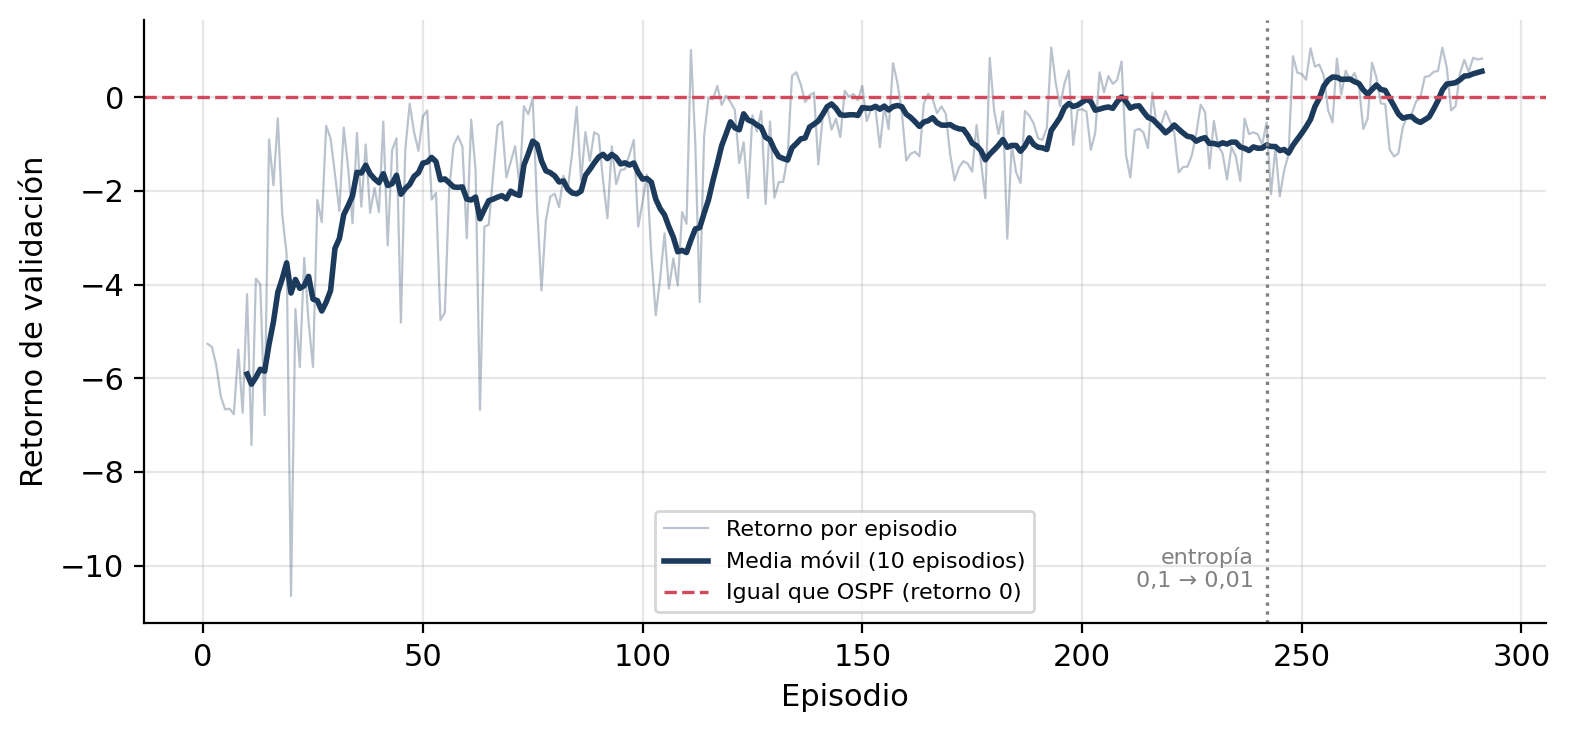
\includegraphics[width=\textwidth]{imagenes/fig_ent_recompensa}
	\caption[Retorno de validación durante el entrenamiento]{Retorno de validación por episodio y su media móvil de 10 episodios. La línea discontinua marca el retorno nulo, que equivale a igualar a OSPF, y la vertical punteada, la reducción del coeficiente de entropía $c_2$ en el episodio 242. El retorno es adimensional y el eje horizontal indica episodios de entrenamiento (iteraciones de PPO).}
	\label{fig:ent_recompensa}
\end{figure}

Al principio del entrenamiento, el retorno medio es de $-5{,}3$: un agente sin entrenar elige caminos casi al azar y termina en configuraciones peores que la de OSPF. A medida que aprende, el retorno crece, y en los mejores episodios supera el cero, con un máximo de $+1{,}06$. Es decir, el número de episodios de entrenamiento no indica cuánto tarda una optimización, sino cuánto tarda el agente en aprender una política cuya configuración final mejora a OSPF de forma consistente; esto solo ocurre en la mayoría de los episodios tras reducir el coeficiente de entropía $c_2$ de la función de pérdida de PPO (Ecuación~\eqref{eq:ppo_loss}), como se analiza en la Sección~\ref{sec:res_entropia}. Además, el retorno y la MLU media de validación están casi perfectamente relacionados (coeficiente de correlación $r = -0{,}998$): los episodios con mayor retorno son, casi sin excepción, los de menor MLU. El término de dispersión añadido no desvía, por tanto, al agente de su objetivo principal, y el retorno es un buen criterio para elegir el modelo.

\subsection{Calidad del enrutamiento durante el entrenamiento}\label{sec:res_mlu_entrenamiento}

La Figura~\ref{fig:ent_mlu} muestra la MLU de validación al final de cada episodio: la media de las 60 matrices y la de la peor de ellas, es decir, la que tiene la MLU más alta en ese episodio.

\begin{figure}[H]
	\centering
	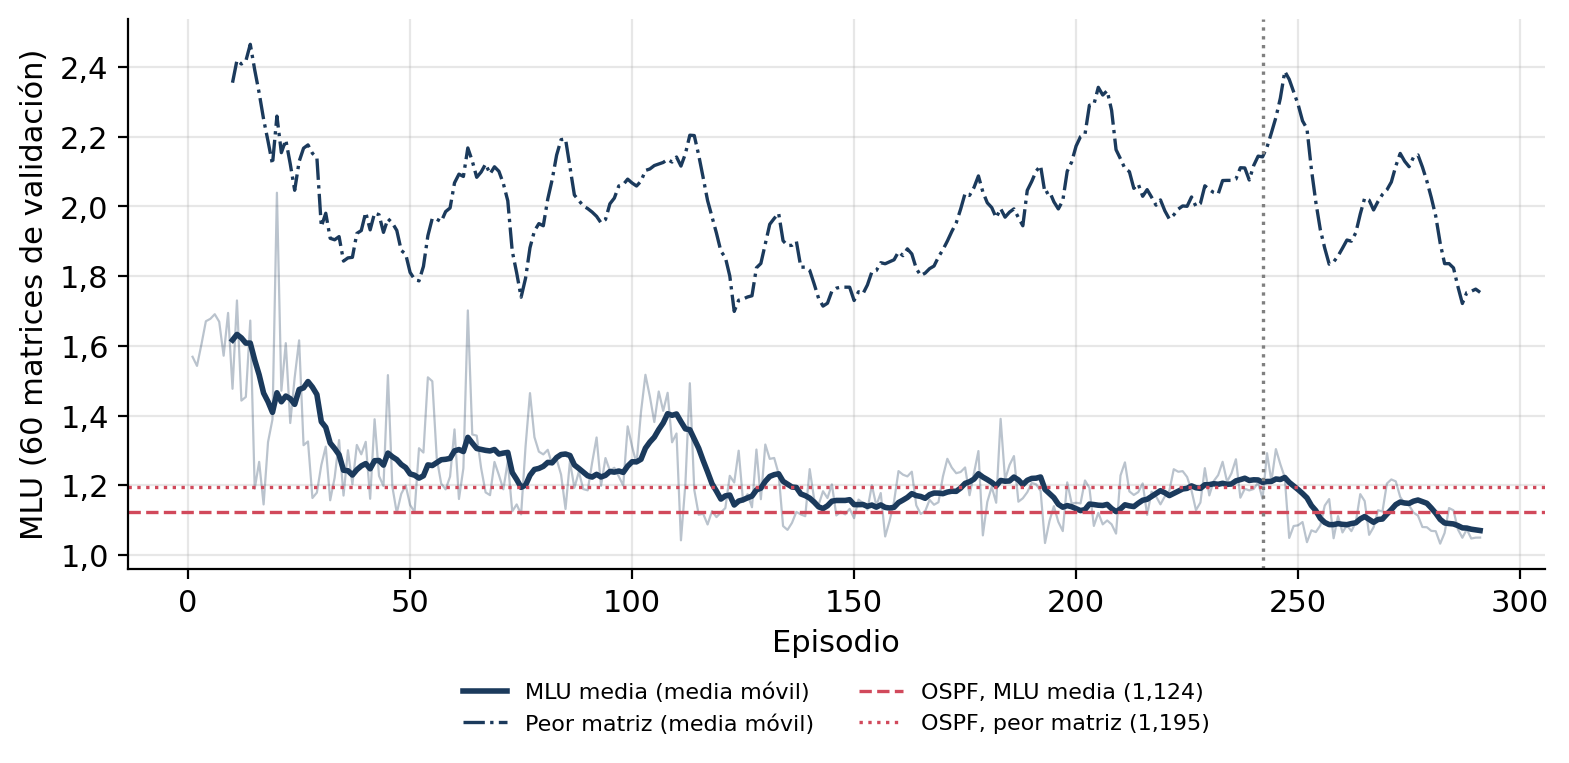
\includegraphics[width=\textwidth]{imagenes/fig_ent_mlu}
	\caption[MLU de validación durante el entrenamiento]{MLU de validación durante el entrenamiento: media de las 60 matrices de validación y MLU de la peor matriz en cada episodio, con su media móvil de 10 episodios, frente a los valores de OSPF (1,124 y 1,195). La MLU es adimensional (carga entre capacidad). La línea vertical marca la reducción del coeficiente de entropía $c_2$.}
	\label{fig:ent_mlu}
\end{figure}

Con OSPF, la MLU media de validación es de 1,124: en promedio, el enlace más cargado recibe un 12\,\% más de tráfico que su capacidad (Sección~\ref{sec:datos}). El agente baja de ese valor a lo largo del entrenamiento, hasta alcanzar 1,033 en el episodio 282, un 8,1\,\% menos. También reduce la dispersión de la carga, de 0,219 con OSPF a unos 0,20, de modo que la MLU no se reduce a costa de desequilibrar el resto de la red.

El comportamiento en el peor caso es distinto. La curva superior de la figura representa, en cada episodio, la MLU de la matriz de validación con mayor MLU al final del episodio, que no es siempre la misma, ya que depende de las decisiones del agente en cada momento. Esta MLU se mantiene por encima de la del peor caso de OSPF (1,195) durante todo el entrenamiento. Es decir, un agente que mejora a OSPF en media puede empeorarlo en matrices concretas. Por este motivo, ENERO conserva siempre la mejor configuración encontrada durante la optimización, que como mínimo es la de OSPF, y la refina después con la LS.

\subsection{Efecto de la reducción de la entropía}\label{sec:res_entropia}

Durante el entrenamiento, la función de pérdida de PPO incluye un término que premia la entropía de la política, es decir, de la distribución de probabilidad que el actor asigna a los nodos intermedios candidatos en cada decisión, ponderado por el coeficiente $c_2$ (Ecuación~\eqref{eq:ppo_loss}). Una entropía alta significa que las probabilidades están repartidas entre muchos candidatos, lo que favorece la exploración; una entropía baja, que el agente concentra la probabilidad en pocos de ellos. La Tabla~\ref{tab:res_entropia} compara el retorno de validación antes y después de reducir $c_2$ de 0,1 a 0,01 en el episodio 242.
\begin{table}[H]
	\centering
	\footnotesize
	\begin{adjustbox}{max width=\textwidth}
	\begin{tabular}{lccc}
		\toprule
		\textbf{Tramo} & \textbf{Episodios} & \textbf{Retorno medio} & \textbf{Episodios con retorno $> 0$} \\
		\midrule
		Entropía $c_2 = 0{,}1$ (últimos 100) & 143--242 & $-0{,}64$ & 19 de 100 (19\,\%) \\
		Entropía $c_2 = 0{,}01$ & 243--291 & $+0{,}02$ & 28 de 49 (57\,\%) \\
		Últimos 10 episodios & 282--291 & $+0{,}55$ & 8 de 10 (80\,\%) \\
		\bottomrule
	\end{tabular}
	\end{adjustbox}
	\caption{Retorno de validación antes y después de reducir el coeficiente de entropía $c_2$ de la política.}
	\label{tab:res_entropia}
\end{table}

Con $c_2 = 0{,}1$, la configuración final del agente mejoraba a OSPF solo en episodios aislados; tras reducir $c_2$, lo hace en la mayoría. Premiar la entropía favorece la exploración, pero introduce aleatoriedad en la política; al reducir su peso, el agente consolida las acciones que mejor funcionan y su comportamiento se vuelve más estable. El mejor retorno, en cambio, apenas cambia: 1,056 en el episodio 282 frente a 1,063 en el 193.

% =====================================================================
\section{Selección del modelo base}\label{sec:res_seleccion}

El episodio 193 obtuvo el mayor retorno de validación de todo el entrenamiento. Sin embargo, en ese momento no era posible saber si el agente seguiría mejorando: el retorno oscila mucho de un episodio a otro y el coeficiente de entropía seguía siendo alto, de modo que la política aún no se había consolidado. Por ello se continuó el entrenamiento, guardando un \textit{checkpoint} en cada episodio, y el modelo se eligió al final comparando los mejores candidatos con datos que no se habían utilizado para seguir el entrenamiento.

Los candidatos fueron el 193, el de mayor retorno antes de reducir la entropía; el 282, con el mayor retorno después de la reducción y la mejor MLU media de todo el entrenamiento; y el 252, otro buen candidato de la fase de entropía baja. Se compararon sobre las matrices 20 a 49 de la partición \texttt{EVALUATE} de las topologías de entrenamiento, que no se habían usado en la validación (que emplea las matrices 0 a 19). La Tabla~\ref{tab:res_seleccion} recoge la mejora sobre OSPF de la etapa DRL con dos criterios: la mejor configuración del episodio, que es la que ENERO conserva, y la configuración al final del episodio.

\begin{table}[H]
	\centering
	\footnotesize
	\begin{adjustbox}{max width=\textwidth}
	\begin{tabular}{lcccc}
		\toprule
		\textbf{Checkpoint} & \textbf{BtAsiaPac} & \textbf{Garr199905} & \textbf{Goodnet} & \textbf{Media} \\
		\midrule
		\multicolumn{5}{l}{\textit{Mejor configuración del episodio}} \\
		193 & 41,1\,\% & 5,1\,\% & 9,6\,\% & 18,6\,\% \\
		282 & 40,4\,\% & 3,9\,\% & 11,6\,\% & 18,6\,\% \\
		252 & 39,7\,\% & 6,1\,\% & 10,4\,\% & 18,8\,\% \\
		\midrule
		\multicolumn{5}{l}{\textit{Configuración al final del episodio}} \\
		193 & 41,0\,\% & $-16{,}6$\,\% & $-2{,}7$\,\% & 7,2\,\% \\
		282 & 36,7\,\% & $-10{,}4$\,\% & $+1{,}4$\,\% & 9,2\,\% \\
		252 & 38,5\,\% & $-15{,}7$\,\% & $-1{,}9$\,\% & 7,0\,\% \\
		\bottomrule
	\end{tabular}
	\end{adjustbox}
	\caption[Mejora sobre OSPF de los checkpoints candidatos]{Mejora de la MLU sobre OSPF de la etapa DRL de los \textit{checkpoints} candidatos, en las matrices 20 a 49 de \texttt{EVALUATE} de las topologías de entrenamiento. Cada \textit{checkpoint} es un modelo ya entrenado que se evalúa sin seguir aprendiendo.}
	\label{tab:res_seleccion}
\end{table}

Con la mejor configuración del episodio, los tres candidatos son prácticamente iguales. La diferencia aparece al final del episodio: el 282 es el que menos empeora y el único que termina por encima de OSPF en Goodnet. Por esa mayor robustez, por tener la mejor MLU media y por proceder de la fase estable del entrenamiento, se eligió el \textit{checkpoint} 282 como modelo base. La comparación deja además dos observaciones útiles:

\begin{itemize}
	\item \textbf{Conservar la mejor configuración es esencial}. En Garr199905, los tres candidatos terminan el episodio peor que OSPF, mientras que su mejor configuración lo mejora: la política acierta en las primeras demandas y deshace después parte de lo conseguido. Este comportamiento es coherente con el factor de descuento $\gamma = 0{,}95$ (Ecuación~\eqref{eq:retorno}), con el que las recompensas del final de un episodio largo tienen poco peso (Sección~\ref{sec:analisis_recompensa}), y justifica el diseño de ENERO.
	\item \textbf{Políticas distintas pueden rendir igual}. Los \textit{checkpoints} 282 y 193 eligen el mismo nodo intermedio en solo el 20--26\,\% de las decisiones en BtAsiaPac y Garr199905, y, sin embargo, obtienen mejoras casi idénticas. Existen muchas formas de desviar el tráfico con resultados muy similares.
\end{itemize}

Conviene distinguir aquí dos costes. El entrenamiento, de unas 87 horas, se realiza una sola vez, con las tres topologías de entrenamiento a la vez (Sección~\ref{sec:hiperparametros_base}), y antes de desplegar el agente, del mismo modo que se diseña cualquier otro sistema antes de ponerlo en servicio. No hay que repetirlo para cada topología: el agente entrenado se aplica directamente, sin volver a entrenar, a cualquier matriz de tráfico y a topologías que no ha visto, como las de las Secciones~\ref{sec:res_calidad} y~\ref{sec:res_mayores}. Los resultados de la Tabla~\ref{tab:res_seleccion} corresponden a esos modelos ya entrenados, que optimizan cada matriz de tráfico nueva sin volver a aprender: en las redes de este tamaño, la etapa DRL tarda unos pocos segundos por matriz y la optimización completa con la LS, del orden de 10 a 20 segundos (Sección~\ref{sec:res_energia}). Esa rapidez en operación es la ventaja que persigue ENERO frente a los métodos clásicos: OSPF no necesita un optimizador centralizado, porque cada enrutador calcula sus caminos de forma distribuida, aunque a cambio de recursos de la red (intercambio de mensajes de estado de enlace) y de un retardo de convergencia; pero no tiene en cuenta la carga y deja una MLU considerablemente peor, y la formulación exacta del enrutamiento por punto intermedio es un problema de programación entera NP-hard, cuyo tiempo de resolución puede crecer rápidamente con el tamaño de la red (Sección~\ref{sec:prog_mat}). La Sección~\ref{sec:res_milp} comprueba si esa ventaja se cumple en las redes evaluadas.

% =====================================================================
\section{Resultados de la compresión en validación}\label{sec:res_compresion}

Esta sección presenta el resultado de cada técnica de compresión durante su propio proceso. Todas las cifras son mejoras de la MLU sobre OSPF de la etapa DRL (Ecuación~\eqref{eq:mejora_ospf}), medidas en las matrices de validación de las topologías de entrenamiento (Sección~\ref{sec:datos}). Con estas matrices, el modelo base obtiene una mejora del 18,1\,\%, que es la referencia de esta sección; la cifra difiere ligeramente del 18,6\,\% de la Tabla~\ref{tab:res_seleccion} porque esta se calculó sobre otras matrices. Estos resultados sirvieron para fijar la configuración de cada técnica; la evaluación definitiva, en topologías no vistas, se presenta en la Sección~\ref{sec:res_calidad}.

\subsection{Poda}\label{sec:res_poda}

La Figura~\ref{fig:poda_barrido} muestra la mejora sobre OSPF del modelo base podado a distintos niveles, sin reentrenar, y la que se obtiene al reentrenar con PPO los niveles del 50 y del 90\,\%. El eje horizontal indica el porcentaje de parámetros del actor que valen cero; como los sesgos y la normalización de capa no se podan, podar el 50\,\% de cada matriz equivale a un 48,4\,\% del total de parámetros, y podar el 90\,\%, a un 87,1\,\%.

\begin{figure}[H]
	\centering
	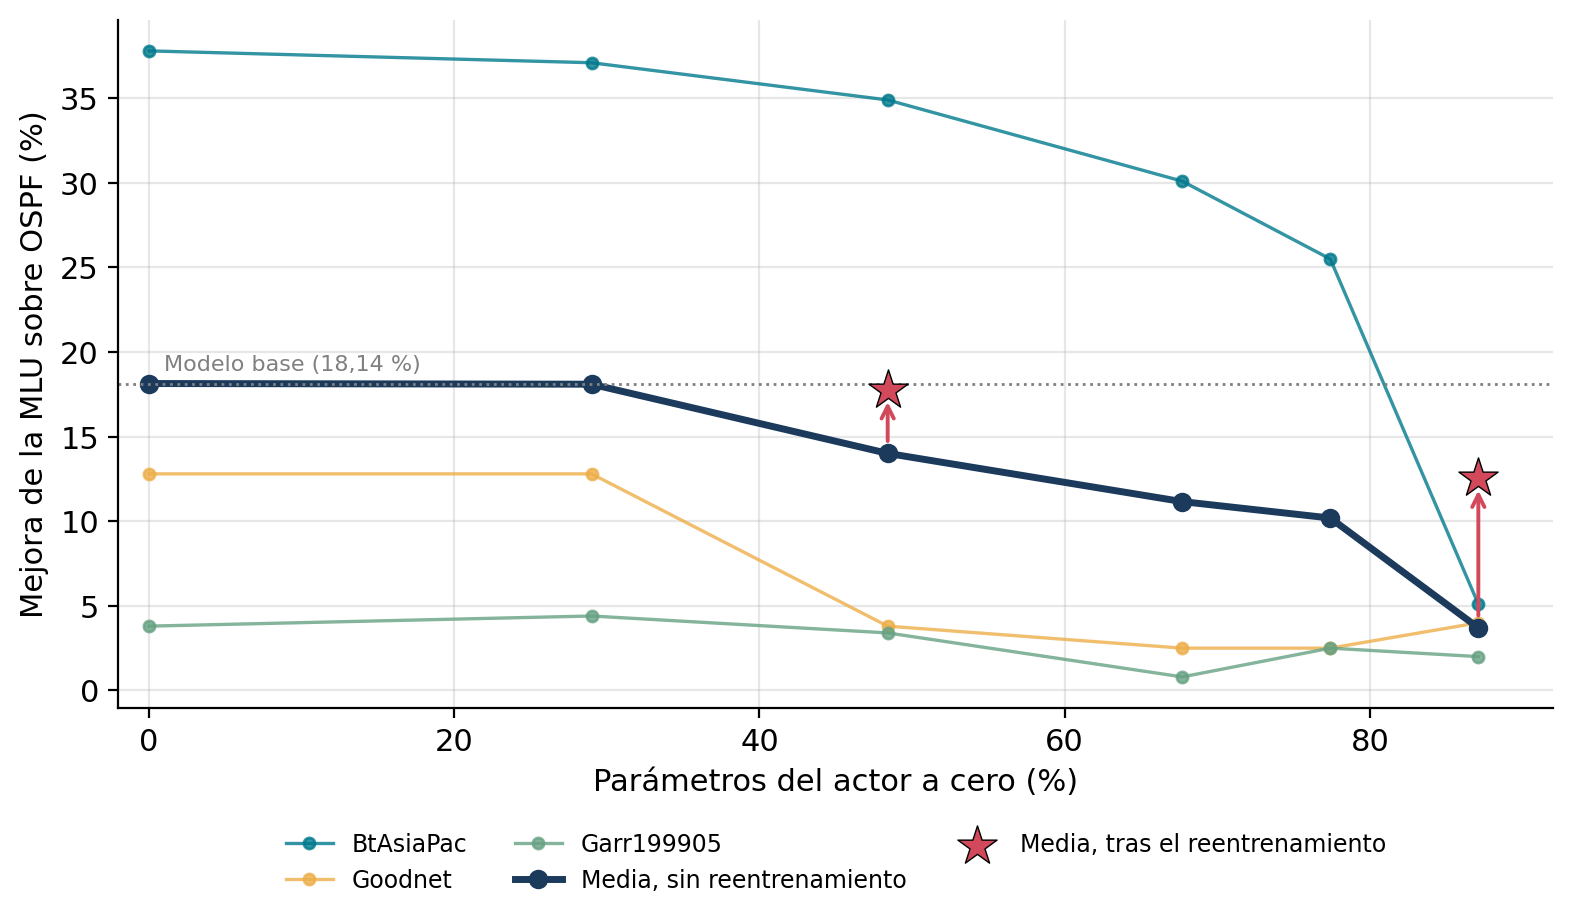
\includegraphics[width=0.95\textwidth]{imagenes/fig_poda_barrido}
	\caption[Mejora sobre OSPF en función del nivel de poda]{Mejora de la MLU sobre OSPF de la etapa DRL en las matrices de validación, en función del porcentaje de parámetros del actor a cero, por topología y en media, sin reentrenamiento. Las estrellas indican la media tras reentrenar los modelos podados al 50 y al 90\,\%.}
	\label{fig:poda_barrido}
\end{figure}

El modelo tiene una redundancia considerable: con un 29\,\% de los parámetros a cero conserva prácticamente toda la mejora del modelo base (18,1\,\%) sin reentrenar. A partir de ese nivel, la calidad disminuye, con un ritmo que depende de la topología. El reentrenamiento recupera la mayor parte de la pérdida: al 50\,\%, la mejora pasa del 14,0 al 17,8\,\%, el 98\,\% de la del modelo base; al 90\,\%, con solo el 13\,\% de los parámetros, pasa del 3,7 al 12,6\,\%, dos tercios de la del modelo base.

\subsection{Cuantización}\label{sec:res_cuantizacion}

La cuantización no requiere reentrenar, por lo que antes de la evaluación completa se comprobó su fidelidad, es decir, cuánto se parecen sus salidas a las del modelo original. Para ello se utilizaron 120 estados obtenidos con matrices de entrenamiento (Sección~\ref{sec:flujo_cuantizacion}) y se midieron dos indicadores: el error absoluto medio de los \textit{logits}, que son las puntuaciones que el actor asigna a cada candidato antes de convertirlas en probabilidades, y el porcentaje de estados en los que el modelo cuantizado elige el mismo candidato que el original. La Tabla~\ref{tab:res_cuantizacion} recoge ambos indicadores junto con el tamaño de cada fichero.

\begin{table}[H]
	\centering
	\footnotesize
	\begin{adjustbox}{max width=\textwidth}
	\begin{tabular}{lcccc}
		\toprule
		\textbf{Variante} & \textbf{Tamaño} & \textbf{Frente a TFLite FP32} & \textbf{Error medio en \textit{logits}} & \textbf{Decisiones iguales} \\
		\midrule
		TFLite FP32 (ref.) & 133,5~KB & -- & 0,00002 & 100\,\% \\
		FP16 & 100,7~KB & $-24{,}6$\,\% & 0,054 & 100\,\% \\
		INT8 dinámico & 80,1~KB & $-40{,}0$\,\% & 2,83 & 76,7\,\% \\
		\bottomrule
	\end{tabular}
	\end{adjustbox}
	\caption[Tamaño y fidelidad de las variantes cuantizadas]{Tamaño y fidelidad de las variantes cuantizadas frente al modelo original, en 120 estados de las topologías de entrenamiento. Los \textit{logits} son adimensionales.}
	\label{tab:res_cuantizacion}
\end{table}

La conversión a TensorFlow Lite no altera el modelo: la variante TFLite FP32, que no está cuantizada, toma las mismas decisiones que el original con un error despreciable, de modo que cualquier diferencia de las otras variantes se debe a la cuantización. FP16 conserva todas las decisiones, mientras que INT8 dinámico cambia una de cada cuatro, con un error medio en los \textit{logits} unas 50 veces mayor que el de FP16. La explicación más probable está en la arquitectura del actor, que aplica ocho veces seguidas las mismas funciones de mensaje y actualización (Sección~\ref{sec:agente}): el error de redondeo introducido en cada iteración se acumula en las siguientes. Las GNN recurrentes parecen, por tanto, más sensibles a la cuantización que las redes con una sola pasada por cada capa.

En cuanto al tamaño, la reducción es menor de lo que sugiere el número de bits. Los pesos del actor ocupan unos 50~KB en FP32, 25~KB en FP16 y 13~KB en INT8, pero los ficheros solo se reducen 1,3 y 1,7 veces respecto a la referencia. El motivo es que un fichero de TensorFlow Lite contiene, además de los pesos, la descripción del grafo de operaciones, en la que las ocho iteraciones del paso de mensajes aparecen desplegadas, y esa parte no se cuantiza. En un modelo tan pequeño, la estructura ocupa más que los pesos; en modelos mucho mayores, en los que los pesos dominan el tamaño, la reducción sería más próxima a la teórica.

\subsection{Destilación}\label{sec:res_destilacion}

La Tabla~\ref{tab:res_destilacion} compara las tres configuraciones de destilación probadas (Sección~\ref{sec:flujo_destilacion}). Para cada una se indica la mejora sobre OSPF de la etapa DRL del mejor estudiante en validación y su proporción respecto a la del maestro, que es el modelo base.

\begin{table}[H]
	\centering
	\footnotesize
	\begin{adjustbox}{max width=\textwidth}
	\begin{tabular}{lcccc}
		\toprule
		\textbf{Configuración} & \textbf{$\alpha$} & \textbf{$\tau$} & \textbf{Mejora del mejor estudiante} & \textbf{Respecto al maestro} \\
		\midrule
		Inicial & 0,7 (con término MSE) & 2 & 13,46\,\% & 74\,\% \\
		Sin MSE & 1 & 2 & 17,83\,\% & 98\,\% \\
		Sin MSE, $\tau = 4$ & 1 & 4 & 18,24\,\% & 100\,\% \\
		\bottomrule
	\end{tabular}
	\end{adjustbox}
	\caption[Resultados de las configuraciones de destilación]{Mejora de la MLU sobre OSPF de la etapa DRL del mejor estudiante de cada configuración, en las matrices de validación. El maestro obtiene un 18,14\,\%.}
	\label{tab:res_destilacion}
\end{table}

La pérdida de destilación combina dos términos (Ecuación~\eqref{eq:kd_total}). El principal, la divergencia KL, mide cuánto se parecen las distribuciones de probabilidad del maestro y del estudiante sobre los candidatos: solo tiene en cuenta qué candidatos prefiere cada modelo y en qué proporción. El auxiliar es el error cuadrático medio (MSE, \textit{Mean Squared Error}): el promedio de los cuadrados de las diferencias entre los \textit{logits} de ambos modelos, es decir, entre los valores numéricos que asignan a cada candidato antes de convertirlos en probabilidades. El peso $\alpha$ reparte la importancia entre ambos.

Con la configuración inicial, $\alpha = 0{,}7$, la pérdida tomaba valores de cientos y oscilaba sin tendencia, el estudiante coincidía con el maestro en solo el 40--55\,\% de las decisiones y su mejora en validación crecía hasta la época 15 y caía después. La causa era el término MSE. Los \textit{logits} del maestro tienen valores grandes, de modo que sus diferencias al cuadrado dominaban la pérdida y obligaban al estudiante a copiar los valores exactos. Pero para decidir solo importa el orden relativo de los \textit{logits}: sumar la misma constante a todos no cambia la decisión. El estudiante, con la mitad de dimensión, no podía reproducir esos valores, y ese objetivo competía con el de la divergencia KL. Al eliminar el MSE ($\alpha = 1$), el estudiante pasa a conservar el 98\,\% de la mejora del maestro.

La temperatura $\tau$ controla cuánto se suavizan las distribuciones antes de compararlas (Ecuación~\eqref{eq:softmax_temp}). Por ejemplo, con \textit{logits} $(5, 4, 1)$, la \textit{softmax} sin suavizar ($\tau = 1$) da probabilidades $(0{,}72,\ 0{,}27,\ 0{,}01)$, mientras que con $\tau = 4$ da $(0{,}47,\ 0{,}36,\ 0{,}17)$: la opción preferida sigue siendo la misma, pero la distribución suavizada indica que la segunda es casi igual de adecuada y que la tercera no es descartable. El maestro, entrenado al final con un coeficiente de entropía bajo, es muy determinista, y con $\tau = 2$ sus distribuciones siguen concentradas casi por completo en un candidato, de modo que aportan poca información sobre los demás. Con $\tau = 4$, el estudiante recibe esa información adicional sobre qué alternativas considera el maestro casi igual de buenas, y su mejora sube de 17,83 a 18,24\,\%. La diferencia es pequeña y está dentro del margen de variación entre ejecuciones, pero va en el sentido esperado. Con esta configuración, el estudiante iguala al maestro en validación con unas 4,6 veces menos parámetros, y es la que se utiliza en el resto del capítulo.

% =====================================================================
\section{Coste de los modelos comprimidos}\label{sec:res_coste}

A partir de esta sección, todos los resultados corresponden al uso de los modelos ya entrenados. La Tabla~\ref{tab:res_coste} recoge el tamaño de cada modelo y su latencia, medida en las topologías de evaluación como la mediana del tiempo de una decisión, es decir, de una llamada al actor con todos los candidatos de una demanda (Sección~\ref{sec:metricas}).

\begin{table}[H]
	\centering
	\footnotesize
	\begin{adjustbox}{max width=\textwidth}
	\begin{tabular}{lrrrrr}
		\toprule
		& & & \textbf{Pesos} & \textbf{Comprimido} & \textbf{Latencia} \\
		\textbf{Modelo} & \textbf{Parámetros} & \textbf{No nulos} & \textbf{(FP32)} & \textbf{(gzip)} & \textbf{mediana} \\
		\midrule
		Original & 12\,737 & 12\,737 & 49,8~KB & 46,0~KB & 16,1~ms \\
		Podado50 & 12\,737 & 6\,577 & 49,8~KB & 28,3~KB & 16,1~ms \\
		Podado90 & 12\,737 & 1\,647 & 49,8~KB & 10,0~KB & 16,1~ms \\
		Estudiante & 2\,753 & 2\,753 & 10,8~KB & 9,9~KB & 5,1~ms \\
		\midrule
		TFLite FP32 & -- & -- & 133,5~KB & 83,5~KB & 72,3~ms \\
		FP16 & -- & -- & 100,7~KB & 50,5~KB & 72,2~ms \\
		INT8 dinámico & -- & -- & 80,1~KB & 27,7~KB & 121,6~ms \\
		\bottomrule
	\end{tabular}
	\end{adjustbox}
	\caption[Tamaño y latencia de los modelos evaluados]{Tamaño y latencia de los modelos evaluados. Para los modelos de TensorFlow Lite, la columna de pesos indica el tamaño del fichero completo. La latencia es la mediana del tiempo por decisión en las tres topologías de evaluación.}
	\label{tab:res_coste}
\end{table}

La poda reduce a la mitad o a la octava parte los parámetros no nulos, pero no el tamaño de las matrices, que conservan los ceros. Su ganancia aparece al almacenar el modelo comprimido: con \texttt{gzip}, el modelo podado al 50\,\% ocupa un 38\,\% menos que el original y el podado al 90\,\%, un 78\,\% menos. En cambio, no reduce la latencia, porque las operaciones de la red multiplican igualmente las matrices completas, incluidos los ceros (Sección~\ref{sec:poda}).

El estudiante es el único modelo que reduce la latencia: con la mitad de dimensión y la mitad de iteraciones, tarda 5,1~ms por decisión frente a los 16,1~ms del original, 3,2 veces menos. La ganancia es mayor cuanto mayor es la topología, porque el coste de cada decisión crece con el número de enlaces y de candidatos (Sección~\ref{sec:drl_te}).

Las variantes de TensorFlow Lite, en cambio, son entre 4,5 y 7,6 veces más lentas que el original ejecutado con TensorFlow. Se comprobó que la diferencia no se debe al número de hilos de cálculo ni a que el intérprete tenga que adaptarse al tamaño de cada entrada: fijando el mismo número de hilos en ambos formatos y midiendo aparte esa adaptación, la diferencia se mantiene. La causa está en la estructura del modelo convertido: las 8 iteraciones del paso de mensajes se despliegan en unas 300 operaciones elementales, porque la activación SELU, la normalización de capa y la celda GRU se descomponen en multiplicaciones, sumas y selecciones, y el intérprete las ejecuta una a una. INT8 dinámico es el más lento porque, además, en cada capa convierte las activaciones a enteros y las devuelve a coma flotante. En este modelo y en este procesador, la cuantización con TensorFlow Lite no aporta velocidad.

% =====================================================================
\section{Calidad del enrutamiento en topologías no vistas}\label{sec:res_calidad}

Esta sección presenta la evaluación principal: todos los modelos, ya entrenados, optimizan las 50 matrices de evaluación de EliBackbone, HurricaneElectric y Janetbackbone, tres topologías que no se han utilizado en ningún momento del entrenamiento, de la compresión ni de la selección de modelos.

\subsection{Resultados globales}

La Tabla~\ref{tab:res_global} resume los resultados medios sobre las 150 matrices. Para cada modelo se indica la mejora de la MLU sobre OSPF (Ecuación~\eqref{eq:mejora_ospf}) que consigue la etapa DRL y la que consigue ENERO completo, es decir, la etapa DRL seguida de la LS (DRL + LS); la distancia de ENERO completo a la cota LP (Ecuación~\eqref{eq:margen_lp}), que indica cuánto le falta para llegar al mínimo teórico y es mejor cuanto menor; y el tiempo medio que tarda en optimizar una matriz. La Figura~\ref{fig:res_mejora} desglosa la mejora por topología.

\begin{table}[H]
	\centering
	\footnotesize
	\setlength{\tabcolsep}{4pt}
	\begin{adjustbox}{max width=\textwidth}
	\begin{tabular}{lcccc}
		\toprule
		& \multicolumn{2}{c}{\textbf{Mejora sobre OSPF}} & \textbf{Distancia a la} & \textbf{Tiempo} \\
		\textbf{Método} & \textbf{DRL} & \textbf{DRL + LS} & \textbf{cota LP (DRL + LS)} & \textbf{por matriz} \\
		\midrule
		Original & 12,6\,\% & 34,3\,\% & 30,7\,\% & 20,0~s \\
		Podado50 & 16,5\,\% & 35,0\,\% & 29,3\,\% & 19,4~s \\
		Podado90 & 5,5\,\% & 32,6\,\% & 34,0\,\% & 21,5~s \\
		Estudiante (media de 4 semillas) & 14,6\,\% & 34,5\,\% & 30,4\,\% & 14,9~s$^{*}$ \\
		TFLite FP32 & 12,6\,\% & 34,3\,\% & 30,7\,\% & 24,8~s \\
		FP16 & 12,7\,\% & 34,5\,\% & 30,4\,\% & 24,9~s \\
		INT8 dinámico & 11,6\,\% & 34,0\,\% & 31,4\,\% & 28,7~s \\
		\midrule
		LS desde OSPF (sin agente) & -- & 31,2\,\% & 36,7\,\% & 17,0~s \\
		\bottomrule
	\end{tabular}
	\end{adjustbox}
	\caption[Resultados medios en las topologías de evaluación]{Resultados medios sobre las 150 matrices de las tres topologías de evaluación. $^{*}$Tiempo del estudiante de la semilla 9, el único medido sin otras cargas en el equipo.}
	\label{tab:res_global}
\end{table}

\begin{figure}[H]
	\centering
	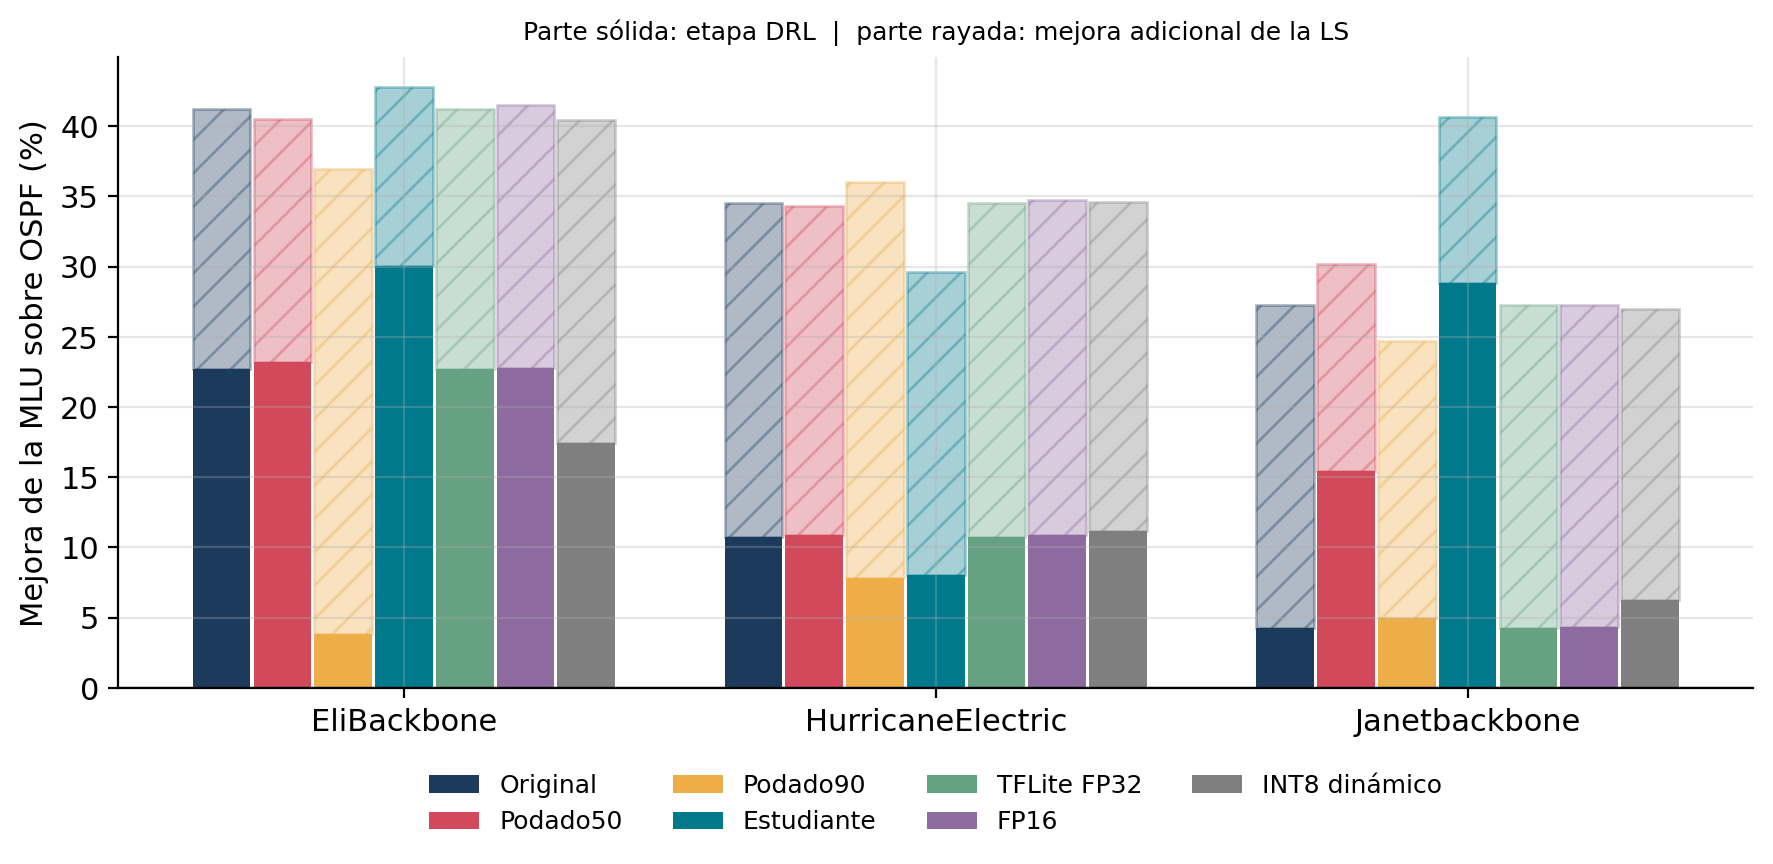
\includegraphics[width=\textwidth]{imagenes/fig_mejora_ospf}
	\caption[Mejora sobre OSPF por topología y modelo]{Mejora media de la MLU sobre OSPF por topología y modelo. La parte sólida de cada barra corresponde a la etapa DRL y la rayada, a lo que añade la LS. El estudiante es el de la semilla 9.}
	\label{fig:res_mejora}
\end{figure}

El resultado principal es que \textbf{la compresión conserva la calidad del enrutamiento}. Con la LS, todos los modelos comprimidos mejoran a OSPF entre un 32,6 y un 35,0\,\% de media, frente al 34,3\,\% del original, y todos superan a la LS aplicada sin agente (31,2\,\%): el agente, comprimido o no, proporciona a la LS un mejor punto de partida.

Para comprobar si las diferencias con el original son reales o se deben a la variabilidad entre matrices, se aplicó la prueba de Wilcoxon a las diferencias de MLU emparejadas por matriz (Sección~\ref{sec:metricas}). El valor $p$ de la prueba es la probabilidad de observar una diferencia al menos tan grande como la medida si ambos modelos fueran igual de buenos; con un valor inferior a 0,05, la diferencia se considera significativa. Para el modelo podado al 50\,\%, FP16 e INT8 dinámico, los valores de $p$ son 0,46, 0,08 y 0,63, de modo que no se observan diferencias estadísticamente significativas entre su calidad y la del original. El modelo podado al 90\,\% es ligeramente peor, con diferencias estadísticamente significativas ($p = 0{,}0008$), aunque la LS compensa casi toda su desventaja en la etapa DRL. La variante TFLite FP32 obtiene exactamente los mismos resultados que el original, lo que confirma la fidelidad de la conversión.\label{sec:res_semillas}

En el caso del estudiante, el primer modelo destilado (semilla 9) obtuvo una mejora del 37,7\,\%, superior a la del original. Para comprobar si ese resultado era estable, la destilación se repitió con otras tres semillas aleatorias, que cambian la inicialización de los pesos del estudiante y el orden en que recibe los datos; no se realizaron más repeticiones porque cada destilación y su evaluación ocupan el equipo varias horas. Los cuatro estudiantes obtienen en validación resultados muy parecidos, entre un 17,0 y un 18,6\,\% de mejora en la etapa DRL, pero en las topologías de evaluación su mejora con LS varía entre el 32,3 y el 37,7\,\%. En media, el estudiante mejora a OSPF un 34,5\,\%, prácticamente lo mismo que el original, y esa es la cifra que figura en la tabla. La destilación conserva, por tanto, la calidad del original reduciendo su latencia 3,2 veces, pero el resultado de un estudiante concreto varía con el entrenamiento, por lo que conviene validarlo en la red en la que se vaya a desplegar.

\subsection{Acuerdo de decisiones}

El acuerdo de decisiones indica en qué porcentaje de las decisiones un modelo comprimido elige el mismo candidato que el original ante el mismo estado (Sección~\ref{sec:metricas}). En las topologías de evaluación es del 99,3\,\% para FP16 y del 53\,\% para INT8 dinámico, pero mucho menor en los modelos cuyos pesos se vuelven a entrenar durante la compresión, siempre con las topologías de entrenamiento y nunca con las de evaluación: del 21\,\% para el podado al 50\,\% y el estudiante, y del 8\,\% para el podado al 90\,\%. A pesar de ello, el podado al 50\,\% no presenta diferencias estadísticamente significativas con el original, el estudiante obtiene en media la misma calidad y el podado al 90\,\% solo es ligeramente peor. Los modelos reentrenados no reproducen las decisiones del original, sino que aprenden su propia política, de calidad similar en media, como ya se vio al comparar los \textit{checkpoints} candidatos (Sección~\ref{sec:res_seleccion}). Por eso un agente comprimido debe evaluarse por la calidad de la tarea completa y no por la fidelidad de sus salidas (Sección~\ref{sec:comp_part}).

\subsection{Generalización y distancia a la cota LP}\label{sec:res_generalizacion}

La etapa DRL del modelo original mejora a OSPF un 12,6\,\% en las topologías de evaluación, frente al 18,6\,\% que obtiene en matrices no utilizadas de las topologías de entrenamiento (Sección~\ref{sec:res_seleccion}). La diferencia se concentra en Janetbackbone, la topología de evaluación más grande, donde la etapa DRL solo mejora a OSPF un 4,3\,\%; aun así, la LS compensa buena parte de la diferencia y ENERO completo mejora a OSPF un 27,3\,\% en esa red. Es la limitación conocida de los agentes entrenados con pocas topologías, que el propio artículo de ENERO señala \cite{ALMASAN2022109166}. En este trabajo se utilizaron las mismas tres topologías de entrenamiento que en el artículo original, porque cada topología adicional alarga el entrenamiento, que en CPU ya requiere cerca de cuatro días. Entre los modelos comprimidos, el único que generaliza claramente peor es el podado al 90\,\%: su etapa DRL conservaba un 12,6\,\% de mejora en validación, pero en las topologías de evaluación se queda en un 5,5\,\%, lo que indica que una poda tan extrema reduce su capacidad de adaptarse a redes nuevas.

La distancia a la cota LP completa este análisis. La cota es la MLU que se obtendría si el tráfico de cada demanda pudiera repartirse libremente entre todos los caminos (Sección~\ref{sec:lp}), algo que ENERO no permite, porque cada demanda sigue un único camino con, como mucho, un nodo intermedio. Es, por tanto, una referencia optimista del margen de mejora, aunque en estas redes resulta ser casi alcanzable: la mejor configuración con un único nodo intermedio por demanda queda a menos de un 0,4\,\% de ella (Sección~\ref{sec:res_milp}). Con el modelo original, ENERO completo queda a un 5\,\% de la cota en EliBackbone, a un 38\,\% en HurricaneElectric y a un 49\,\% en Janetbackbone, siempre más cerca que la LS sin agente (14, 40 y 56\,\%). En la red más pequeña, ENERO se encuentra muy próximo al límite teórico, mientras que en las mayores queda un margen de mejora que podría aprovecharse entrenando con topologías más parecidas a ellas o resolviendo el problema de forma exacta (Sección~\ref{sec:res_milp}).

% =====================================================================
\section{Evaluación en redes mayores}\label{sec:res_escalabilidad}\label{sec:res_tipo_red}\label{sec:res_mayores}

Para comprobar si las conclusiones se mantienen en redes más grandes y distintas de las de entrenamiento, se evaluaron las siete topologías adicionales, de 30 a 43 nodos, con 10 matrices cada una (Sección~\ref{sec:datos}). La Tabla~\ref{tab:res_escal} recoge la mejora sobre OSPF de ENERO completo con cada modelo, junto con la de la LS sin agente y la de la cota LP. Esta última es la mejora máxima teórica, que ningún método puede superar. El grado medio de cada red es el número medio de enlaces por nodo, una medida de la densidad de su estructura; las topologías de evaluación principales tienen un grado medio de 3,0 a 3,1.

\begin{table}[H]
	\centering
	\footnotesize
	\setlength{\tabcolsep}{3.5pt}
	\begin{adjustbox}{max width=\textwidth}
	\begin{tabular}{lcc|ccccc|cc}
		\toprule
		& & \textbf{Grado} & \multicolumn{5}{c|}{\textbf{ENERO completo (DRL + LS)}} & \textbf{LS sin} & \textbf{Cota} \\
		\textbf{Topología} & \textbf{Nodos} & \textbf{medio} & \textbf{Original} & \textbf{Estudiante} & \textbf{Podado50} & \textbf{Podado90} & \textbf{INT8} & \textbf{agente} & \textbf{LP} \\
		\midrule
		WideJpn & 30 & 2,2 & 18,7\,\% & 18,9\,\% & 18,7\,\% & 18,7\,\% & 18,7\,\% & 18,7\,\% & 36,8\,\% \\
		GtsPoland & 33 & 2,2 & 15,7\,\% & 15,0\,\% & 14,9\,\% & 15,2\,\% & 15,6\,\% & 15,0\,\% & 35,2\,\% \\
		Bics & 33 & 2,9 & 25,1\,\% & 24,6\,\% & 26,3\,\% & 21,4\,\% & 22,2\,\% & 16,3\,\% & 29,6\,\% \\
		Evolink & 37 & 2,4 & 9,4\,\% & 9,2\,\% & 9,4\,\% & 9,4\,\% & 9,4\,\% & 9,3\,\% & 16,8\,\% \\
		Cesnet200511 & 39 & 2,3 & 19,9\,\% & 18,8\,\% & 19,3\,\% & 18,1\,\% & 20,9\,\% & 18,0\,\% & 50,3\,\% \\
		LambdaNet & 42 & 2,2 & 11,1\,\% & 10,6\,\% & 11,3\,\% & 9,6\,\% & 10,4\,\% & 10,6\,\% & 17,1\,\% \\
		Sanet & 43 & 2,1 & 13,7\,\% & 14,0\,\% & 12,8\,\% & 13,9\,\% & 13,0\,\% & 14,4\,\% & 15,2\,\% \\
		\midrule
		\textbf{Media} & & & \textbf{16,2\,\%} & \textbf{15,9\,\%} & \textbf{16,1\,\%} & \textbf{15,2\,\%} & \textbf{15,7\,\%} & \textbf{14,6\,\%} & \textbf{28,7\,\%} \\
		\bottomrule
	\end{tabular}
	\end{adjustbox}
	\caption[Resultados en las redes mayores]{Mejora media de la MLU sobre OSPF de ENERO completo (DRL + LS) en las siete redes mayores, con 10 matrices por topología, junto con la de la LS sin agente y la de la cota LP, que es la máxima teórica. El grado medio es el número medio de enlaces por nodo. El estudiante es el de la semilla 9.}
	\label{tab:res_escal}
\end{table}

La primera conclusión es que \textbf{la compresión sigue siendo robusta en redes mayores}. En las 70 matrices, el estudiante y el modelo podado al 50\,\% siguen sin presentar diferencias estadísticamente significativas con el original ($p = 0{,}92$ y $0{,}64$ en la prueba de Wilcoxon), y las diferencias del podado al 90\,\% y de INT8 dinámico son pequeñas, de un punto porcentual o menos de media. Los modelos comprimidos se comportan, por tanto, como el original también fuera de las topologías de evaluación principales.

La Tabla~\ref{tab:res_escal} permite ver también cuánto se acerca ENERO al límite teórico en estas redes. Con el modelo original, obtiene de media el 56\,\% de la mejora máxima posible (16,2 frente a 28,7\,\%), con valores que van desde el 40\,\% de Cesnet200511 hasta el 90\,\% de Sanet. A diferencia de lo observado en las topologías de evaluación principales, en las que la distancia a la cota crece con el tamaño de la red (Sección~\ref{sec:res_generalizacion}), aquí no se aprecia una tendencia clara con el número de nodos: la red más grande, Sanet, es la que queda más cerca de la cota.

La segunda conclusión se refiere al propio agente: \textbf{su aportación depende de lo parecida que sea la red a las de entrenamiento}. En Bics, la única de las nuevas con un grado medio cercano a 3, como las de evaluación y dos de las tres de entrenamiento, ENERO mejora a la LS sin agente en casi 9 puntos porcentuales (25,1 frente a 16,3\,\%). En las otras seis, más dispersas (grado medio de 2,1 a 2,4), la diferencia es pequeña y la mayor parte de la mejora la consigue la LS. La Figura~\ref{fig:res_tipo_red} lo resume para las diez topologías.

\begin{figure}[H]
	\centering
	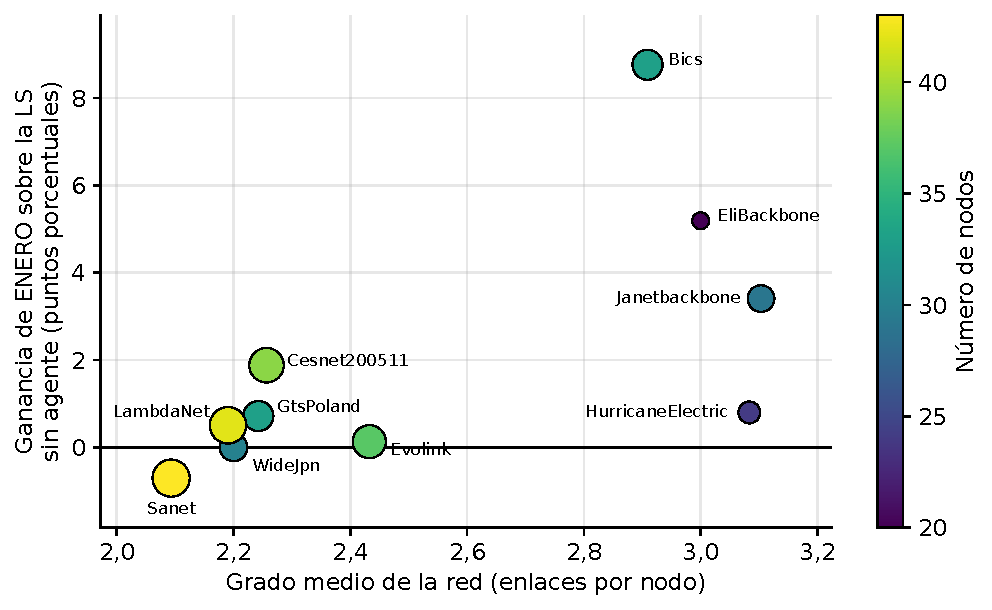
\includegraphics[width=\textwidth]{imagenes/fig_tipo_red}
	\caption[Aportación de ENERO según el grado medio de la red]{Diferencia, en puntos porcentuales, entre la mejora sobre OSPF de ENERO completo (modelo original) y la de la LS sin agente, frente al grado medio de cada topología. Un valor positivo indica que el agente mejora el resultado de la LS. El tamaño y el color de cada punto indican el número de nodos.}
	\label{fig:res_tipo_red}
\end{figure}

El par formado por Bics y GtsPoland, ambas con 33 nodos y con un grado medio de 2,9 y 2,2, respectivamente, indica que lo determinante es la estructura de la red más que su tamaño: en la primera ENERO aporta 8,8 puntos sobre la LS, y en la segunda, 0,7. Con pocas topologías por grupo y 10 matrices en las nuevas, esta conclusión es orientativa, pero coincide con lo que cabe esperar de un agente entrenado con solo tres redes pequeñas (17 a 23 nodos), dos de ellas con grado medio de 3 o más: generaliza bien a redes de su tipo y peor a redes distintas. En consecuencia, para desplegar ENERO en un tipo de red concreto, conviene entrenarlo, o al menos ajustarlo, con topologías de ese tipo, y comprimirlo después.

En cuanto al tiempo, el de ENERO crece con el tamaño de la red, desde unos 8~s por matriz en EliBackbone a entre 85 y 145~s en las redes de 39 a 43 nodos, porque aumentan a la vez el número de demandas críticas, el de candidatos y el coste de cada iteración de la LS. En estas redes, la LS ocupa casi todo el tiempo, de modo que la menor latencia del estudiante apenas se aprecia en el total (141 frente a 145~s en Cesnet200511): la compresión del agente es más útil cuanto mayor es el peso de la etapa DRL en la optimización.

% =====================================================================
\section{Tiempo de optimización e impacto energético}\label{sec:res_energia}

\subsection{Reparto del tiempo de optimización}

La Figura~\ref{fig:res_tiempos} desglosa el tiempo medio de optimización de una matriz en las tres topologías de evaluación entre la etapa DRL, que incluye la construcción de los grafos de los candidatos y las llamadas al actor, y la LS.

\begin{figure}[H]
	\centering
	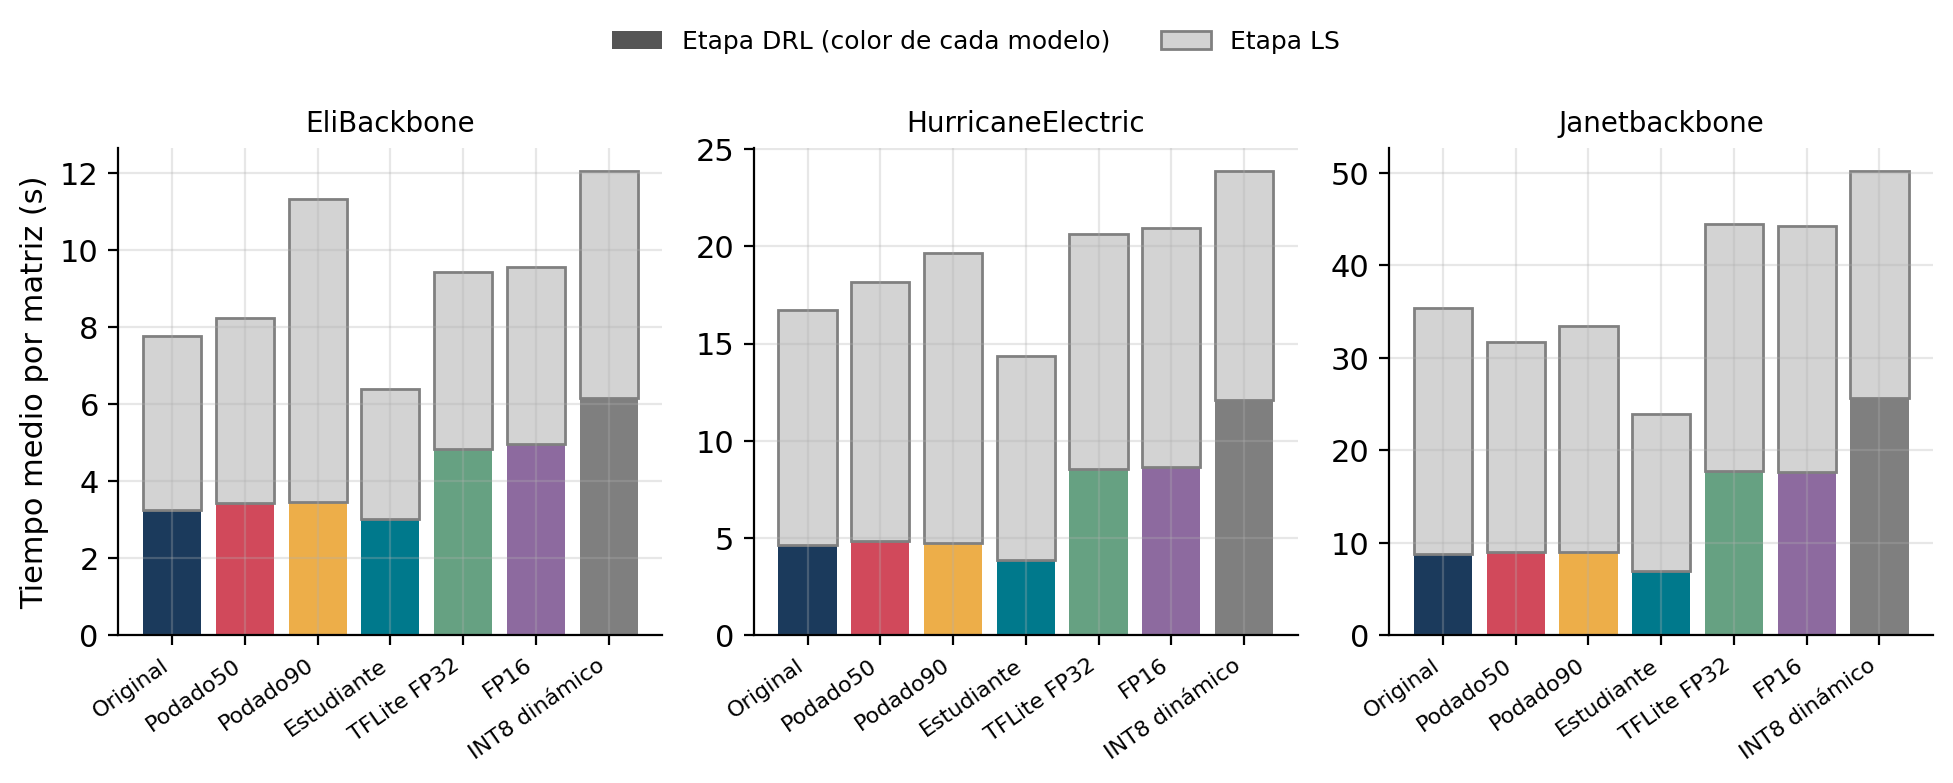
\includegraphics[width=\textwidth]{imagenes/fig_tiempos}
	\caption[Reparto del tiempo de optimización]{Tiempo medio de optimización de una matriz de tráfico, en segundos, repartido entre la etapa DRL y la LS, para cada modelo, en las tres topologías de evaluación. El estudiante es el de la semilla 9.}
	\label{fig:res_tiempos}
\end{figure}

Con los modelos de TensorFlow, la LS ocupa entre el 69 y el 73\,\% del tiempo total, y la etapa DRL, entre 4,6 y 5,8~s por matriz. Dentro de esta etapa, la inferencia de la red es solo una parte: la mayor parte del tiempo se dedica a construir los grafos de los candidatos y a simular la red en Python. Por ello, acelerar la red neuronal tiene un efecto limitado sobre el tiempo total.

El estudiante reduce el tiempo total entre un 5 y un 25\,\%. El 5\,\% se debe a su menor latencia, que reduce la etapa DRL de 5,6 a 4,6~s por matriz, y lo consigue cualquier estudiante. Cuando, además, proporciona a la LS un mejor punto de partida, como el de la semilla 9, esta necesita menos iteraciones para converger (27 frente a 43 en Janetbackbone, donde el tiempo total se reduce en torno a un tercio), y el ahorro medio en las tres topologías alcanza el 25\,\%.

\subsection{Impacto energético}

La Tabla~\ref{tab:res_energia} estima la energía de cada optimización con la Ecuación~\eqref{eq:energia}, como el producto de la potencia media del procesador medida durante el entrenamiento (23,9~W, Sección~\ref{sec:costes_energia}) por el tiempo de optimización de una matriz. Para dar una idea del consumo en operación, la extrapola a un año suponiendo una optimización cada 5 minutos.

\begin{table}[H]
	\centering
	\footnotesize
	\setlength{\tabcolsep}{4pt}
	\begin{adjustbox}{max width=\textwidth}
	\begin{tabular}{lccccc}
		\toprule
		& \textbf{Tiempo} & \textbf{Tiempo total} & \textbf{Energía por} & \textbf{Energía} & \textbf{Frente al} \\
		\textbf{Método} & \textbf{etapa DRL} & \textbf{por matriz} & \textbf{optimización} & \textbf{anual} & \textbf{original} \\
		\midrule
		Original & 5,56~s & 19,96~s & 477~J & 13,9~kWh & -- \\
		Podado50 & 5,78~s & 19,37~s & 463~J & 13,5~kWh & $-3$\,\% \\
		Podado90 & 5,75~s & 21,46~s & 513~J & 15,0~kWh & $+8$\,\% \\
		Estudiante (semilla 9) & 4,61~s & 14,89~s & 356~J & 10,4~kWh & $-25$\,\% \\
		TFLite FP32 & 10,39~s & 24,85~s & 594~J & 17,3~kWh & $+25$\,\% \\
		FP16 & 10,44~s & 24,94~s & 596~J & 17,4~kWh & $+25$\,\% \\
		INT8 dinámico & 14,64~s & 28,70~s & 686~J & 20,0~kWh & $+44$\,\% \\
		\bottomrule
	\end{tabular}
	\end{adjustbox}
	\caption[Energía estimada por optimización y anual]{Tiempo medio por matriz en las topologías de evaluación y energía estimada por optimización y por año (una optimización cada 5 minutos, $N_{\text{ejec}} = 105\,120$), con una potencia de 23,9~W.}
	\label{tab:res_energia}
\end{table}

Las cifras absolutas son pequeñas, porque corresponden a un único optimizador en un procesador de bajo consumo; lo relevante son las diferencias relativas, que se multiplican cuando el optimizador se ejecuta en muchos controladores o con mayor frecuencia. El estudiante es la única variante que reduce el consumo de forma apreciable, entre un 5 y un 25\,\% según la calidad del punto de partida que proporcione a la LS. La poda apenas modifica el consumo, y la cuantización con TensorFlow Lite lo aumenta en este procesador, porque alarga el tiempo de optimización. La estimación utiliza la potencia de la CPU bajo carga sostenida, por lo que es aproximada; la comparación entre modelos, que depende sobre todo de los tiempos medidos, es más fiable que los valores absolutos.

Estas cifras permiten también comparar la energía que se consume una sola vez con la que se ahorra en operación (Sección~\ref{sec:costes_energia}). El entrenamiento del agente base consumió unos 2,1~kWh en el procesador (23,9~W durante unas 87 horas). Con una optimización cada 5 minutos, el ahorro del estudiante igualaría esa energía en unos siete meses en el mejor caso (ahorro del 25\,\%) y en unos tres años en el peor (5\,\%). El coste que añade realmente la compresión es el de la destilación, que ocupa el equipo solo unas horas, por lo que se amortiza mucho antes.

% =====================================================================
\section{Comparación con la formulación exacta}\label{sec:res_milp}

Las secciones anteriores comparan cada modelo comprimido con el original, y muestran que la compresión reduce su coste sin empeorar el enrutamiento. Queda por responder una pregunta previa desde el punto de vista práctico: si ENERO, original o comprimido, es una buena forma de resolver este problema. Para ello se compara con las dos variantes de la formulación exacta MILP del enrutamiento por punto intermedio (Sección~\ref{sec:milp}), sobre las mismas matrices y en el mismo equipo. La Tabla~\ref{tab:res_milp} recoge la mejora sobre OSPF y el tiempo por matriz de cada método en las diez topologías, y la Figura~\ref{fig:res_calidad_tiempo} los representa de forma conjunta. De los modelos comprimidos se incluye el estudiante, que es el más rápido; el resto obtiene una calidad y unos tiempos similares a los del original (Secciones~\ref{sec:res_calidad} y~\ref{sec:res_energia}).

\begin{table}[H]
	\centering
	\footnotesize
	\setlength{\tabcolsep}{4pt}
	\begin{adjustbox}{max width=\textwidth}
	\begin{tabular}{lccccc}
		\toprule
		& \textbf{ENERO} & \textbf{ENERO} & \textbf{MILP} & \textbf{MILP} & \textbf{Cota} \\
		\textbf{Topología} & \textbf{original} & \textbf{estudiante} & \textbf{demandas críticas} & \textbf{todas las demandas} & \textbf{LP} \\
		\midrule
		EliBackbone & 41,3 (7,8) & 42,8 (6,4) & 41,5 (0,39) & 44,0 (9,5) & 44,1 \\
		HurricaneElectric & 34,5 (16,7) & 29,6 (14,4) & 41,2 (0,16) & 52,5 (9,8) & 52,7 \\
		Janetbackbone & 27,3 (35,4) & 40,6 (23,9) & 38,1 (0,31) & 51,0 (10,1) & 51,1 \\
		\textit{Media} & 34,3 (20,0) & 37,7 (14,9) & 40,3 (0,28) & 49,2 (9,8) & 49,3 \\
		\midrule
		WideJpn & 18,7 (42,1) & 18,9 (40,1) & 24,1 (0,20) & 36,8 (0,53) & 36,8 \\
		GtsPoland & 15,7 (32,8) & 15,0 (40,5) & 27,3 (4,3) & 35,1 (10,0) & 35,2 \\
		Bics & 25,1 (34,9) & 24,6 (31,1) & 26,6 (0,86) & 29,6 (8,7) & 29,6 \\
		Evolink & 9,4 (50,1) & 9,2 (47,2) & 10,8 (0,24) & 16,8 (2,2) & 16,8 \\
		Cesnet200511 & 19,9 (145,4) & 18,8 (141,1) & 37,0 (0,08) & 50,1 (4,8) & 50,3 \\
		LambdaNet & 11,1 (86,4) & 10,6 (86,5) & 15,2 (0,47) & 17,1 (8,8) & 17,1 \\
		Sanet & 13,7 (87,9) & 14,0 (91,6) & 15,2 (0,80) & 15,1 (10,1) & 15,2 \\
		\textit{Media} & 16,2 (68,5) & 15,9 (68,3) & 22,3 (0,99) & 28,7 (6,5) & 28,7 \\
		\bottomrule
	\end{tabular}
	\end{adjustbox}
	\caption[Comparación de ENERO con la formulación exacta MILP]{Mejora media de la MLU sobre OSPF (\%) y, entre paréntesis, tiempo medio por matriz (s) de ENERO completo (DRL + LS) con el modelo original y con el estudiante de la semilla 9, y de las dos variantes del MILP con un límite de 10~s, en las tres topologías de evaluación principales (50 matrices cada una) y en las siete redes mayores (10 matrices cada una). La última columna es la mejora máxima teórica que da la cota LP.}
	\label{tab:res_milp}
\end{table}

\begin{figure}[H]
	\centering
	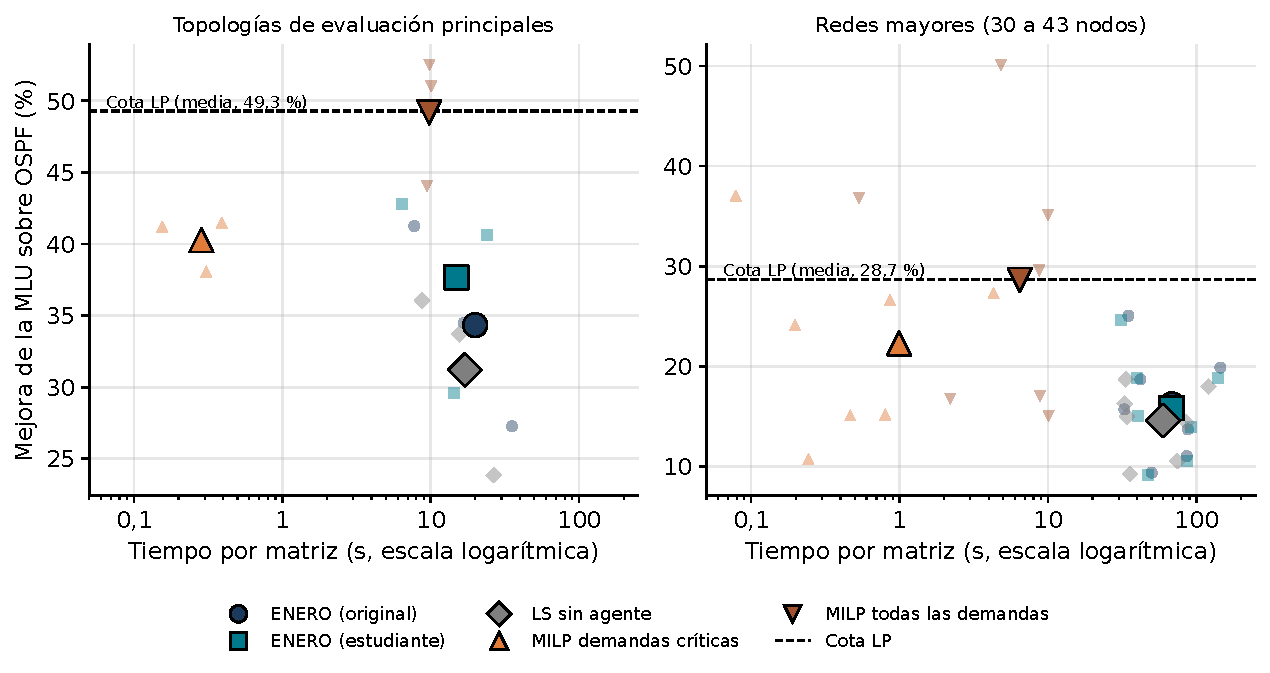
\includegraphics[width=\textwidth]{imagenes/fig_calidad_tiempo}
	\caption[Calidad frente a tiempo de optimización de cada método]{Mejora de la MLU sobre OSPF frente al tiempo por matriz, en escala logarítmica, de ENERO (modelo original y estudiante), la LS sin agente y las dos variantes del MILP. Los puntos pequeños corresponden a cada topología y los grandes, a la media de cada método. La línea discontinua marca la mejora media de la cota LP en cada grupo de redes.}
	\label{fig:res_calidad_tiempo}
\end{figure}

El primer resultado se refiere a la calidad. \textbf{El MILP sobre las demandas críticas mejora a ENERO original en las diez topologías}: un 40,3\,\% de media en las topologías principales y un 22,3\,\% en las redes mayores, frente al 34,3 y el 16,2\,\% de ENERO, que además aplica la LS. Como este MILP decide las mismas demandas que la etapa DRL, su resultado es el que obtendría el agente con una política perfecta, y la diferencia con ENERO mide cuánto se aleja de ese óptimo la política aprendida. Esa diferencia es pequeña en las redes parecidas a las de entrenamiento, como EliBackbone o Bics, y muy grande en las demás: en Cesnet200511, el MILP mejora a OSPF un 37,0\,\% y ENERO, un 19,9\,\%. Es la misma pauta de generalización observada en la Sección~\ref{sec:res_mayores}, ahora medida frente a un óptimo y no frente a la LS. El estudiante de la semilla 9 es el único modelo que supera a este MILP, en EliBackbone y Janetbackbone. Es posible porque la LS vuelve a seleccionar las demandas críticas a partir de la configuración que entrega la etapa DRL, de modo que puede modificar demandas que el MILP mantiene en su camino de OSPF.

El MILP sobre todas las demandas obtiene un 49,2\,\% de mejora media en las topologías principales y un 28,7\,\% en las mayores, prácticamente lo mismo que la cota LP (49,3 y 28,7\,\%). En todas las redes queda a menos de un 0,4\,\% de ella. Por tanto, en estas redes la restricción de un único nodo intermedio por demanda apenas limita la calidad, como apuntaban los resultados previos sobre el enrutamiento por segmentos \cite{bhatia2015optimized}, y casi toda la distancia entre ENERO y la cota LP (Sección~\ref{sec:res_generalizacion}) se debe al método de optimización y no al esquema de enrutamiento.

El segundo resultado se refiere al tiempo. \textbf{El MILP sobre las demandas críticas tarda de media 0,28~s por matriz en las topologías principales y 0,99~s en las redes mayores, unas 70 veces menos que ENERO} (20,0 y 68,5~s). Con el límite de 10~s, alcanzó el óptimo demostrado en 67 de las 70 matrices de las redes mayores; las tres restantes, en GtsPoland, quedaron a menos de un 0,2\,\% de la cota inferior que da el \textit{solver}, y con 60~s también se resolvieron de forma óptima. El MILP sobre todas las demandas tiene unas siete veces más variables y tarda más, 9,8 y 6,5~s de media, pero sigue siendo más rápido que ENERO en todas las redes salvo EliBackbone, la más pequeña. En las redes mayores agota el límite de 10~s en 37 de las 70 matrices; aun así, sus soluciones quedan a menos de un 0,5\,\% de la cota inferior, y con 60~s alcanza el óptimo en 60 de ellas, con 18,8~s de media. Este comportamiento es una ventaja práctica del método exacto: aunque se detenga antes de terminar, entrega una solución válida e indica cuánto puede alejarse del óptimo, algo que ENERO no proporciona. Como el tiempo del MILP no incluye la construcción del modelo en Python (Sección~\ref{sec:milp}), la comparación favorece algo al método exacto, pero la diferencia con ENERO es de casi dos órdenes de magnitud. Tampoco la compresión la reduce de forma apreciable: el estudiante, el modelo más rápido, sigue tardando entre 50 y 70 veces más que el MILP sobre las demandas críticas, y obtiene peor resultado que él en ocho de las diez redes.

El tercer resultado se refiere al coste de puesta en marcha y a la aplicabilidad. ENERO necesita un entrenamiento previo de unas 87 horas en CPU, a lo que se suma el de la compresión, y su calidad depende de que la red se parezca a las de entrenamiento: para desplegarlo en un tipo de red distinto habría que volver a entrenarlo o ajustarlo. El MILP no necesita entrenamiento; se construye a partir de la topología y de la matriz de tráfico de cada momento, por lo que se aplica igual a cualquier red y se adapta de forma inmediata a cambios en la topología. La diferencia también se refleja en la energía. Con el mismo modelo de la Sección~\ref{sec:res_energia}, una optimización con el MILP sobre las demandas críticas consume unos 7~J en las topologías principales, frente a los 477~J de ENERO original y los 356~J del estudiante, lo que supone unos 0,2~kWh al año frente a 13,9 y 10,4~kWh. Solo la energía del entrenamiento del agente base (unos 2,1~kWh) bastaría para más de diez años de optimizaciones con el MILP. La cifra es orientativa, porque la potencia del procesador durante la resolución puede diferir de la medida en el entrenamiento, pero la diferencia es lo bastante grande para no depender de ese detalle.

La ventaja del método exacto tiene un límite. El número de variables del MILP crece con el número de demandas y de candidatos, y el tiempo de resolución de un problema entero puede crecer de forma exponencial con su tamaño (Sección~\ref{sec:prog_mat}). Ese crecimiento ya se aprecia en la variante de todas las demandas, que agota el límite de 10~s en parte de las matrices de cinco de las siete redes mayores. Las redes evaluadas tienen como máximo 43 nodos, así que este trabajo no permite afirmar a partir de qué tamaño el MILP dejaría de resolverse en un tiempo razonable, que es donde un agente entrenado podría resultar competitivo.

En conjunto, \textbf{en las redes evaluadas, la formulación exacta es preferible a ENERO, original o comprimido, en calidad, en tiempo por optimización y en coste de puesta en marcha}. La compresión cumple su objetivo, ya que reduce el coste del agente sin empeorar el enrutamiento, pero no cambia esta comparación, porque la desventaja de ENERO no está en el tamaño de la red neuronal, sino en el propio enfoque de aprendizaje.

% =====================================================================
\section{Síntesis de resultados y recomendaciones}\label{sec:res_sintesis}

La Tabla~\ref{tab:res_sintesis} resume los efectos de cada técnica frente al modelo original en las topologías de evaluación principales.

\begin{table}[H]
	\centering
	\footnotesize
	\setlength{\tabcolsep}{4pt}
	\begin{adjustbox}{max width=\textwidth}
	\begin{tabular}{l>{\raggedright\arraybackslash}p{2.9cm}>{\raggedright\arraybackslash}p{2.1cm}>{\raggedright\arraybackslash}p{3.0cm}>{\raggedright\arraybackslash}p{1.6cm}}
		\toprule
		& \textbf{Tamaño} & \textbf{Latencia} & \textbf{Calidad (DRL + LS)} & \textbf{Energía} \\
		\midrule
		Podado50 & $-38$\,\% (gzip) & Sin cambio & Sin diferencias significativas & $-3$\,\% \\
		Podado90 & $-78$\,\% (gzip) & Sin cambio & Ligeramente peor, diferencia significativa ($-1{,}7$ puntos) & $+8$\,\% \\
		FP16 & $-25$\,\% (frente a TFLite FP32) & 4,5 veces mayor & Sin diferencias significativas & $+25$\,\% \\
		INT8 dinámico & $-40$\,\% (frente a TFLite FP32) & 7,6 veces mayor & Sin diferencias significativas & $+44$\,\% \\
		Estudiante & $-78$\,\% de parámetros & 3,2 veces menor & Similar en media & $-5$ a $-25$\,\% \\
		\bottomrule
	\end{tabular}
	\end{adjustbox}
	\caption{Síntesis de los efectos de cada técnica de compresión frente al modelo original.}
	\label{tab:res_sintesis}
\end{table}

La destilación es la técnica que mejor se adapta a este problema: es la única que reduce la latencia en un procesador de propósito general, porque modifica la arquitectura y no solo la representación de los pesos, y conserva en media la calidad del original, también en redes mayores. Su principal limitación es que el resultado de un estudiante concreto varía con el entrenamiento, por lo que conviene validarlo antes de desplegarlo. La poda moderada reduce el almacenamiento sin pérdida de calidad, pero sus beneficios en tiempo requerirían hardware capaz de aprovechar los ceros. La cuantización reduce el tamaño del fichero, pero en un modelo tan pequeño la ganancia es limitada y, con TensorFlow Lite, aumenta el tiempo de ejecución en este procesador.

En función del tipo de red, los resultados permiten orientar la elección:
\begin{itemize}
	\item \textbf{En redes parecidas a las de entrenamiento} (grado medio en torno a 3 y tamaño similar), el agente mejora claramente a la LS y su compresión resulta útil: con poda moderada si la restricción es el almacenamiento, o con destilación si lo es la latencia.
	\item \textbf{En redes mayores o más dispersas}, todos los modelos comprimidos rinden como el original, pero el agente aporta menos sobre la LS. Antes de comprimirlo convendría entrenarlo con topologías de ese tipo.
	\item \textbf{Si la restricción es el almacenamiento o la distribución del modelo}, el estudiante es la opción más compacta sin pérdida de calidad (9,9~KB comprimido), seguido de INT8 dinámico y de la poda al 50\,\% (27,7 y 28,3~KB).
\end{itemize}

Estas recomendaciones indican cómo comprimir el agente si se opta por ENERO. Sin embargo, al valorar los métodos no solo por la calidad del enrutamiento, sino también por su aplicabilidad práctica, la conclusión es otra: \textbf{en redes de hasta unas decenas de nodos, como las evaluadas, la metodología más adecuada es la formulación exacta (Sección~\ref{sec:res_milp}). El MILP sobre las demandas críticas es la opción más práctica, porque resuelve de forma óptima el problema de la etapa DRL en menos de un segundo y sin entrenamiento previo; el MILP sobre todas las demandas es preferible si prima la calidad, ya que alcanza prácticamente la cota LP en unos segundos. ENERO y sus versiones comprimidas solo podrían tener interés en redes mucho mayores, en las que el método exacto deje de resolverse en un tiempo razonable.}

%
\chapter{Conclusiones}\label{cap:con}

El trabajo partía de una pregunta: si se puede reducir de forma apreciable el coste de ejecutar un agente DRL+GNN para ingeniería de tráfico sin empeorar el enrutamiento que produce. Para responderla se puso en marcha el agente de ENERO con bibliotecas actuales, se entrenó un agente base con una recompensa corregida, se le aplicaron poda, cuantización y destilación, y los modelos resultantes se evaluaron en tres topologías que no habían intervenido en ningún momento del proceso y, después, en siete redes mayores. Para valorar el alcance práctico de los resultados, ENERO, original y comprimido, se comparó además con la formulación exacta del mismo problema. Este capítulo recoge lo que se ha aprendido (Sección~\ref{sec:con_conclusiones}), con qué límites (Sección~\ref{sec:con_limitaciones}), qué quedaría por hacer (Sección~\ref{sec:con_futuro}) y una valoración personal (Sección~\ref{sec:con_valoracion}).

% =====================================================================
\section{Conclusiones}\label{sec:con_conclusiones}

La respuesta es que sí: el coste del agente se puede reducir de forma importante sin empeorar el enrutamiento, aunque cada técnica lo consigue en un aspecto distinto y su beneficio depende del hardware y del tipo de red. Sin embargo, la comparación con la formulación exacta lleva a una conclusión de mayor alcance, que se recoge al final de esta sección: en las redes estudiadas, ni ENERO ni sus versiones comprimidas son la mejor forma de resolver este problema.

La primera conclusión es que \textbf{la compresión conserva la calidad del enrutamiento}. En las 150 matrices de las tres topologías de evaluación, todos los modelos comprimidos, seguidos de la LS, mejoran la MLU de OSPF entre un 32,6 y un 35,0\,\% de media, frente al 34,3\,\% del modelo original, y todos superan a la LS aplicada sin agente. El modelo podado al 50\,\% y las variantes FP16 e INT8 de rango dinámico no presentan diferencias estadísticamente significativas con el original, y el estudiante obtiene en media la misma calidad; solo la poda extrema, al 90\,\%, es ligeramente peor, con diferencias estadísticamente significativas. El resultado se mantiene en las siete redes mayores, donde los modelos comprimidos siguen rindiendo como el original.

La segunda es que \textbf{la destilación es la técnica más adecuada para un procesador convencional}. El estudiante tiene 4,6 veces menos parámetros y es el único modelo que acelera la inferencia, 3,2 veces, porque reduce la arquitectura y no solo la forma de guardar los pesos. Conserva en media la calidad del original y reduce entre un 5 y un 25\,\% el tiempo y la energía de cada optimización, según la calidad del punto de partida que entregue a la LS. Al repetir la destilación con varias semillas se vio que el resultado de un estudiante concreto varía de un entrenamiento a otro, por lo que conviene validarlo en la red de destino antes de desplegarlo. El estudio de configuraciones mostró también que, para destilar este agente, conviene comparar solo las distribuciones de probabilidad del maestro y del estudiante, con una temperatura alta, y no sus valores numéricos.

La tercera es que \textbf{la poda y la cuantización reducen el tamaño, pero no el tiempo, en un procesador convencional}. El agente tiene bastante redundancia: casi un tercio de sus pesos se pueden eliminar sin reentrenar y, reentrenando, el modelo podado a la mitad conserva el 98\,\% de la mejora del original y ocupa un 38\,\% menos comprimido. Pero la poda no estructurada solo acelera con hardware que aproveche los ceros. La cuantización con TensorFlow Lite reduce el fichero entre un 25 y un 40\,\%, aunque en un modelo tan pequeño el grafo de operaciones ocupa más que los pesos, y en este procesador resulta más lenta que TensorFlow porque el modelo convertido se ejecuta operación a operación.

La cuarta es que \textbf{en ENERO la red neuronal no es el cuello de botella}. La LS ocupa en torno al 70\,\% del tiempo de optimización, y dentro de la etapa DRL pesa más construir los grafos de los candidatos y simular la red que la inferencia. Comprimir el agente mejora sobre todo la parte que depende de él, y la calidad de la solución que entrega a la LS influye tanto como su velocidad.

La quinta conclusión es que \textbf{el agente aporta más en redes parecidas a las de entrenamiento}. En las topologías con una estructura similar, ENERO mejora claramente a la LS sin agente y queda cerca del óptimo de su propio espacio de búsqueda; en redes mayores y más dispersas, su aportación es menor y se aleja mucho de ese óptimo. Si se utiliza ENERO, la recomendación práctica es entrenar o ajustar el agente con topologías del tipo en que se va a desplegar y comprimirlo después: con poda moderada si importa el almacenamiento, o con destilación si importa la latencia.

La sexta es que \textbf{el acuerdo de decisiones no sirve para medir la calidad de un agente comprimido}. Modelos que coinciden con el original en una de cada cinco decisiones obtienen una calidad similar, porque hay muchas formas casi igual de buenas de desviar el tráfico. A diferencia de lo habitual al comprimir clasificadores, la evaluación debe hacerse sobre la tarea completa.

Por último, la conclusión de mayor alcance se refiere a la metodología. Tras evaluar ENERO y sus versiones comprimidas no solo por la calidad del enrutamiento, sino también por su aplicabilidad práctica (el tiempo de cada optimización, el coste de entrenar y ajustar el agente y su capacidad de generalizar a redes distintas), \textbf{la metodología más adecuada para redes de hasta unas decenas de nodos es la formulación exacta del enrutamiento por punto intermedio como MILP}. Resuelto sobre las mismas demandas críticas que el agente, el MILP obtiene el óptimo del problema que aborda ENERO en menos de un segundo de media, unas 70 veces más rápido, con mejor resultado que ENERO original en las diez redes evaluadas y sin entrenamiento previo. Resuelto sobre todas las demandas, alcanza prácticamente la cota de programación lineal en unos segundos. El aprendizaje por refuerzo profundo, en cambio, requiere días de entrenamiento, generaliza mal a redes distintas de las de entrenamiento y, precisamente en esas redes, queda lejos del óptimo. La compresión reduce el coste del agente, pero no cambia esta conclusión, porque la desventaja de ENERO no está en el tamaño de su red neuronal, sino en el enfoque. Su posible interés queda limitado a redes mucho mayores, en las que el método exacto deje de resolverse en un tiempo razonable, algo que este trabajo no ha podido comprobar.

En cuanto a los objetivos de la Sección~\ref{sec:int_objetivos}, se ha revisado el estado del arte, se ha migrado ENERO a Gymnasium y entrenado un agente base en CPU, se ha corregido la recompensa, se han aplicado las tres familias de compresión y se han evaluado con una metodología que separa el coste de la red del de la optimización completa e incluye la cota de programación lineal, el acuerdo de decisiones y contrastes estadísticos emparejados. También se ha estimado el impacto energético de cada alternativa y se ha comparado ENERO, original y comprimido, con la formulación exacta del problema, en calidad y en aplicabilidad práctica.

% =====================================================================
\section{Limitaciones}\label{sec:con_limitaciones}

Las conclusiones anteriores deben leerse teniendo en cuenta las siguientes limitaciones:

\begin{itemize}
	\item \textbf{Simulación y hardware}. Todo se ha hecho en simulación y en un único procesador de propósito general. En hardware con soporte para operaciones dispersas o aritmética entera, la poda y la cuantización podrían comportarse de otra forma, y la cuantización solo se ha probado con TensorFlow Lite.
	\item \textbf{Pocas topologías de entrenamiento}. El agente se entrena con tres topologías, lo que limita su generalización a redes de otro tipo. Las siete redes mayores se evaluaron con 10 matrices cada una, de modo que las conclusiones sobre ellas son orientativas. Esta limitación se debe al tiempo disponible.
	\item \textbf{Variabilidad entre entrenamientos}. Solo se ha medido para la destilación, con cuatro semillas, porque cada repetición ocupa el equipo varias horas. El agente base y la poda corresponden a un único entrenamiento.
	\item \textbf{Ajuste limitado de hiperparámetros}. Los hiperparámetros se fijaron tras pocas pruebas por el coste de cada entrenamiento en CPU.
	\item \textbf{Tamaño de las redes y otros optimizadores}. Las redes evaluadas tienen como máximo 43 nodos. En ellas el MILP se resuelve en segundos, pero no se ha comprobado cómo crece su tiempo en redes de cientos de nodos, que es donde un agente entrenado podría compensar. Tampoco se ha comparado con otros optimizadores, como DEFO, y el tiempo medido del MILP no incluye la construcción del modelo.
	\item \textbf{Estimación energética}. La energía se estima con la potencia media de la CPU bajo carga y los tiempos medidos, sin medir el consumo durante cada evaluación.
\end{itemize}

% =====================================================================
\section{Trabajo futuro}\label{sec:con_futuro}

De los resultados y de las limitaciones se desprenden varias líneas de trabajo:

\begin{itemize}
	\item \textbf{Entrenar para la red de destino}. Entrenar o ajustar el agente con topologías del tipo en que se va a desplegar, y comprobar que la compresión conserva esa mejora, es el paso más directo para aumentar su aportación en redes grandes o dispersas.
	\item \textbf{Combinar técnicas}. Podar o cuantizar el estudiante destilado podría acumular beneficios, y destilar hacia estudiantes aún más pequeños permitiría localizar el límite de capacidad del modelo.
	\item \textbf{Poda estructurada}. Eliminar neuronas o dimensiones completas del estado, en lugar de pesos sueltos, produce modelos densos más pequeños que sí se aceleran en cualquier hardware.
	\item \textbf{Otros motores de inferencia}. Probar la cuantización con motores que fusionen las operaciones del grafo, o en hardware con aritmética entera, donde debería aparecer su ventaja en velocidad.
	\item \textbf{Más topologías y semillas}. Repetir con varias semillas el agente base y la poda, y buscar un criterio de validación que permita anticipar qué estudiante generalizará mejor.
	\item \textbf{Escalabilidad del MILP y enfoques híbridos}. Medir el tiempo del MILP en redes de cientos de nodos, para localizar el tamaño a partir del cual un agente entrenado podría compensar, y estudiar enfoques que combinen ambos métodos: usar la solución del agente como punto de partida del MILP, o usar las soluciones del MILP para entrenar o destilar el agente.
	\item \textbf{Acelerar el resto del optimizador}. Como la red no es el cuello de botella, hay margen en la construcción de los grafos, la simulación de la red y la LS, por ejemplo vectorizándolas o limitando la búsqueda a los candidatos mejor valorados por el agente.
	\item \textbf{Porcentaje de demandas críticas}. Estudiar cómo influye el porcentaje de demandas críticas en la calidad y en el tiempo de optimización según el tamaño de la red, y si conviene adaptarlo a cada topología.
\end{itemize}

% =====================================================================
\section{Valoración personal}\label{sec:con_valoracion}

Cuando empecé el trabajo apenas conocía el aprendizaje por refuerzo y las redes neuronales de grafos (solo por encima), y no tenía claro cómo encajaban en la gestión de una red. Entender ENERO desde el artículo hasta el código me obligó a juntar cosas que en el grado había visto en asignaturas distintas: enrutamiento, optimización y aprendizaje automático.

Lo que más tiempo me ha llevado no ha sido la compresión, sino conseguir que todo lo demás funcionara bien. Algunos errores no daban ningún fallo visible: la primera evaluación de los modelos de TensorFlow Lite les pasaba un solo grafo en lugar de los de todos los candidatos, y el agente elegía siempre la primera acción sin que nada lo indicara; el sesgo de la recompensa solo apareció al revisar el entorno línea a línea. Corregirlos obligó a repetir buena parte del trabajo en septiembre y octubre, pero ahora puedo defender cada cifra de la memoria.

También he tenido que aprender a planificar con experimentos que duran días. Con un portátil con GPU no compatible, con el procesador a unos 95~$^\circ$C durante días enteros, cada entrenamiento había que pensarlo bien antes de lanzarlo, trocearlo para poder reanudarlo cuando se cortaba y repartir el trabajo entre dos equipos.

Por último, me quedo con que algunos resultados no salieron como esperaba. El primer estudiante destilado parecía mejor que su maestro, y solo al repetir la destilación con otras semillas vi que el resultado variaba de un entrenamiento a otro; me ha enseñado a no fiarme de un único entrenamiento. Tampoco esperaba que la red neuronal no fuera el cuello de botella del optimizador, y eso me hizo entender que, para valorar una técnica de compresión, hay que medirla dentro del sistema completo y no solo sobre el modelo.

Lo que más me ha hecho reflexionar ha sido la comparación con el MILP. Empecé el trabajo dando por hecho que un agente entrenado era la forma más moderna y eficaz de resolver este problema, y me costó aceptar un resultado que no favorecía al método que estaba estudiando. Me ha enseñado que una comparación entre métodos tiene que hacerse sin ideas preconcebidas, y que un resultado negativo, si está bien medido, tiene tanto valor como uno positivo.

%
\appendix
%
\chapter{Topologías de evaluación}\label{anx:topologias}
La Figura~\ref{fig:estructura_redes_evaluacion} muestra la estructura de las tres topologías de la evaluación principal (Tabla~\ref{tab:topologias}).

\begin{figure}[H]
	\centering
	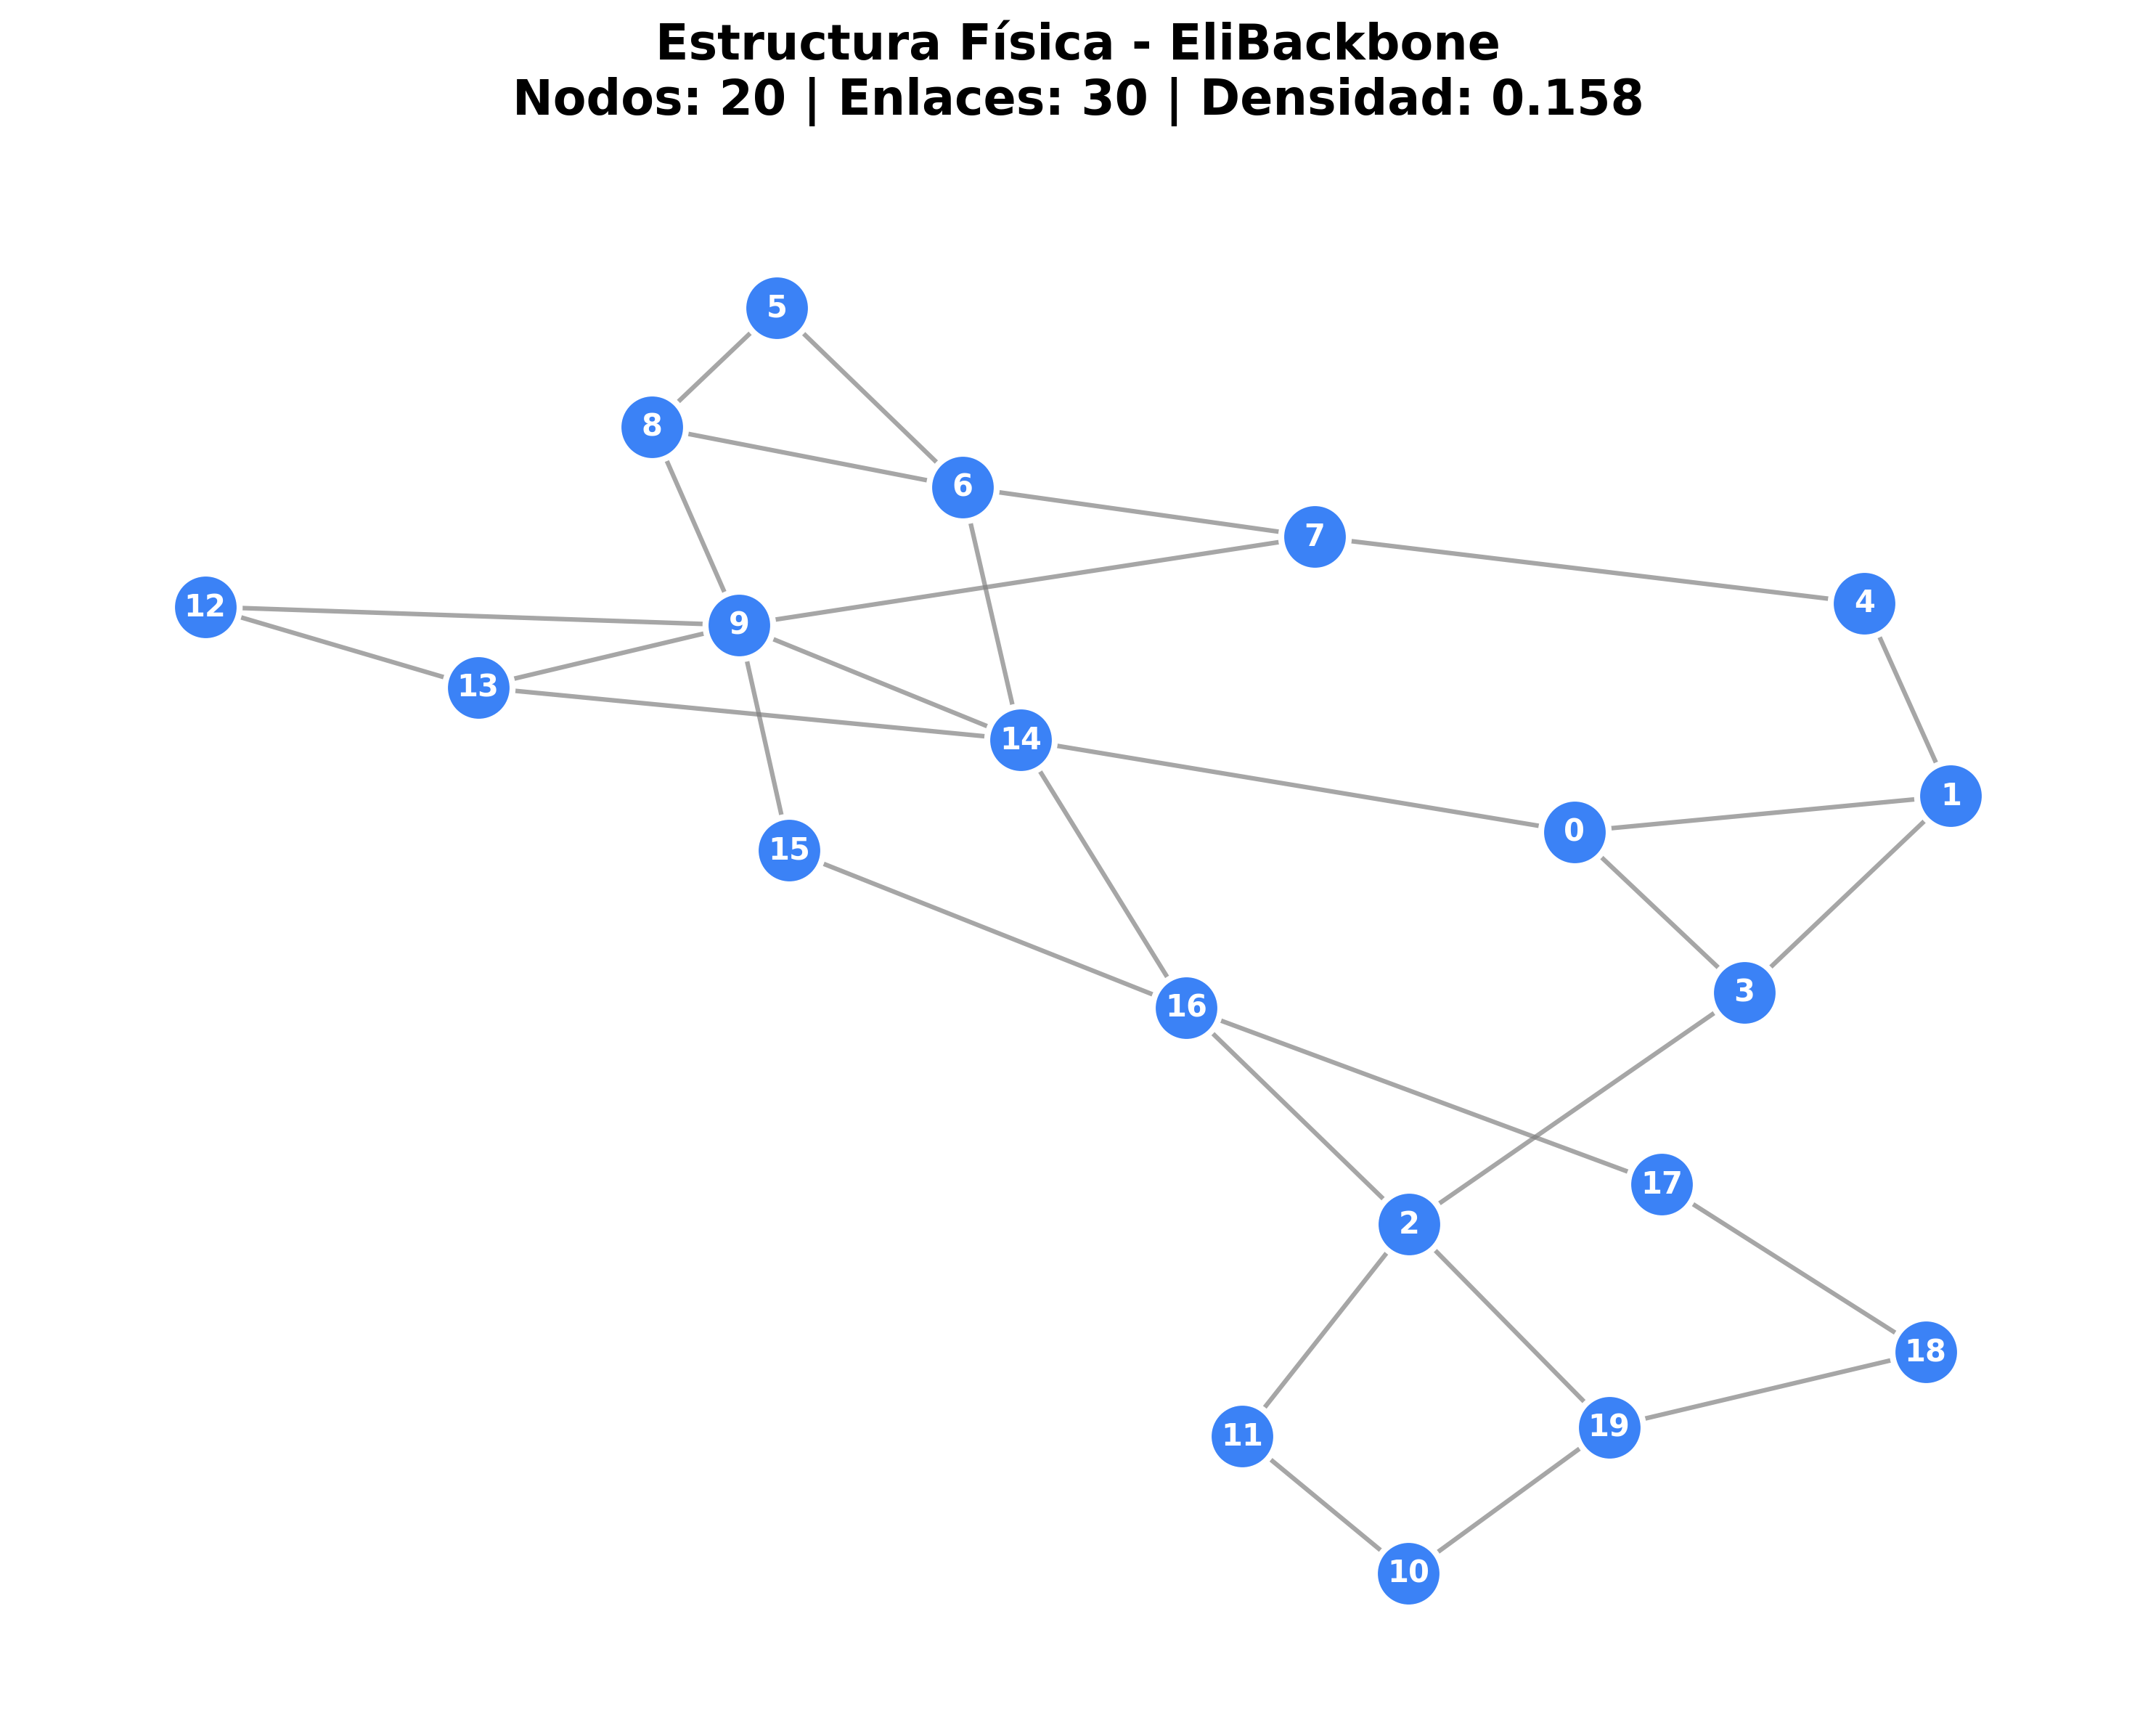
\includegraphics[width=0.5\textwidth]{imagenes/EliBackbone_estructura.png}\\[2mm]
	{\small (a) EliBackbone}\\[4mm]
	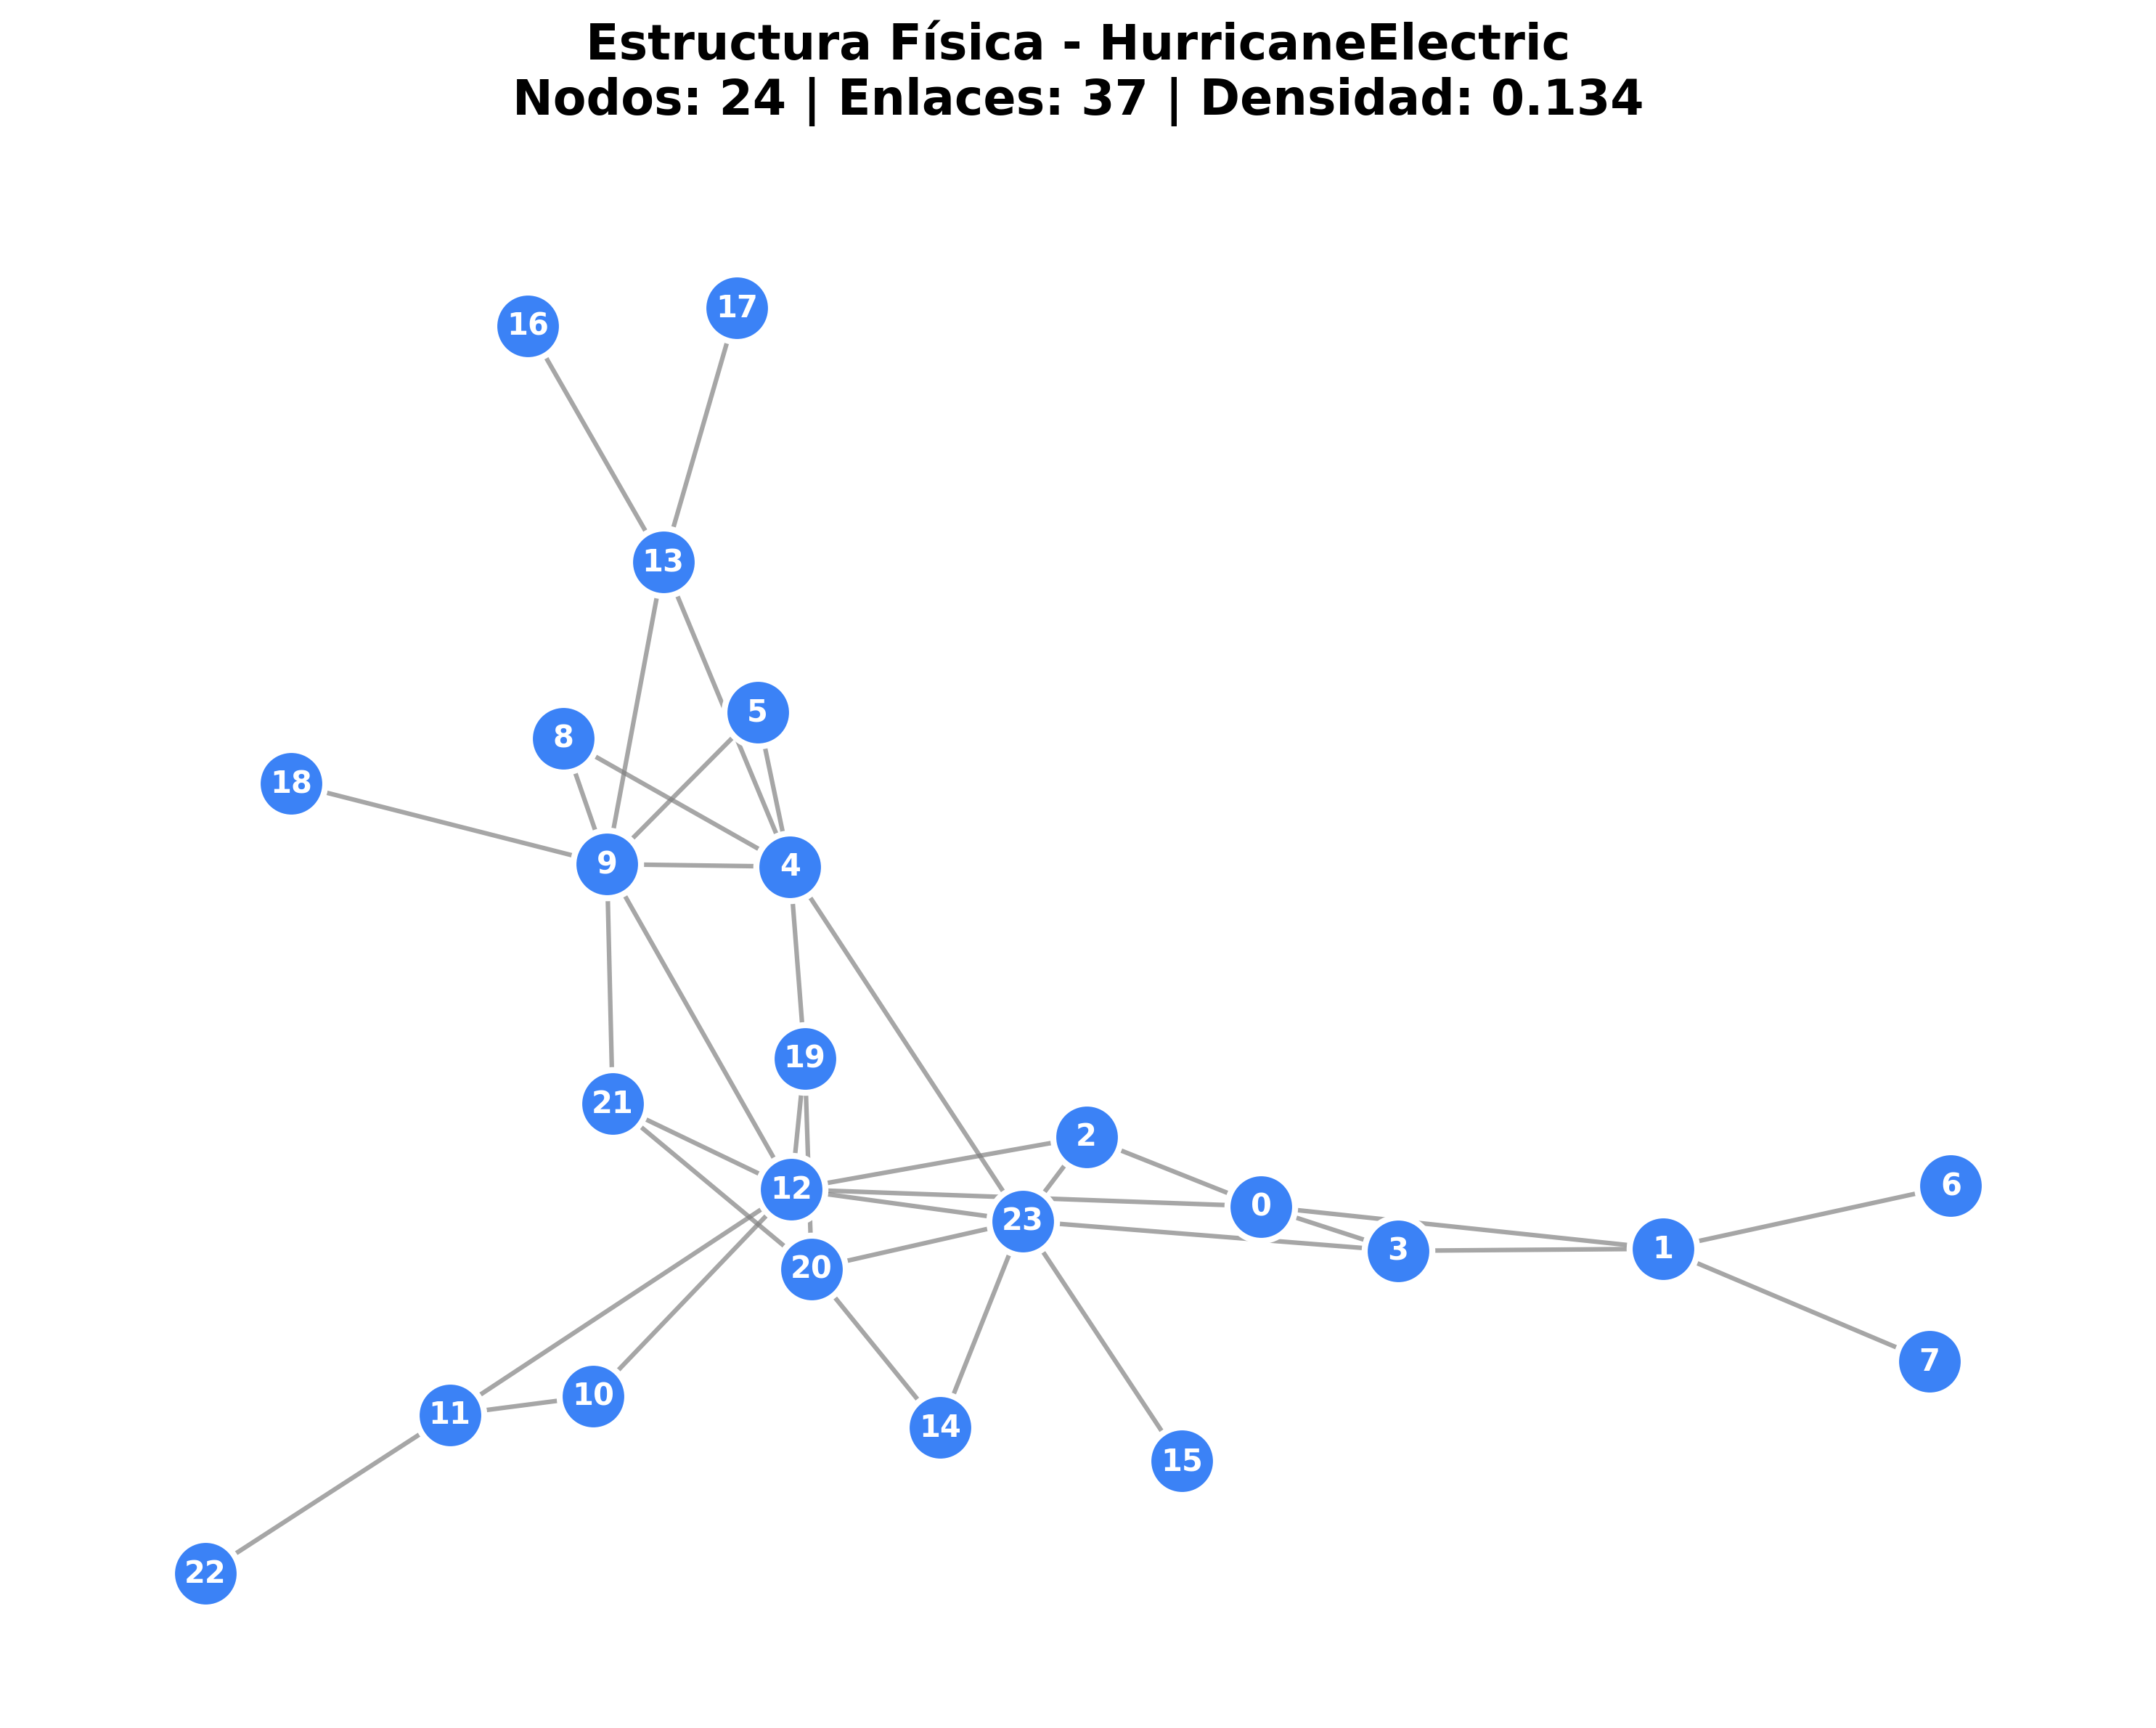
\includegraphics[width=0.5\textwidth]{imagenes/HurricaneElectric_estructura.png}\\[2mm]
	{\small (b) HurricaneElectric}\\[4mm]
	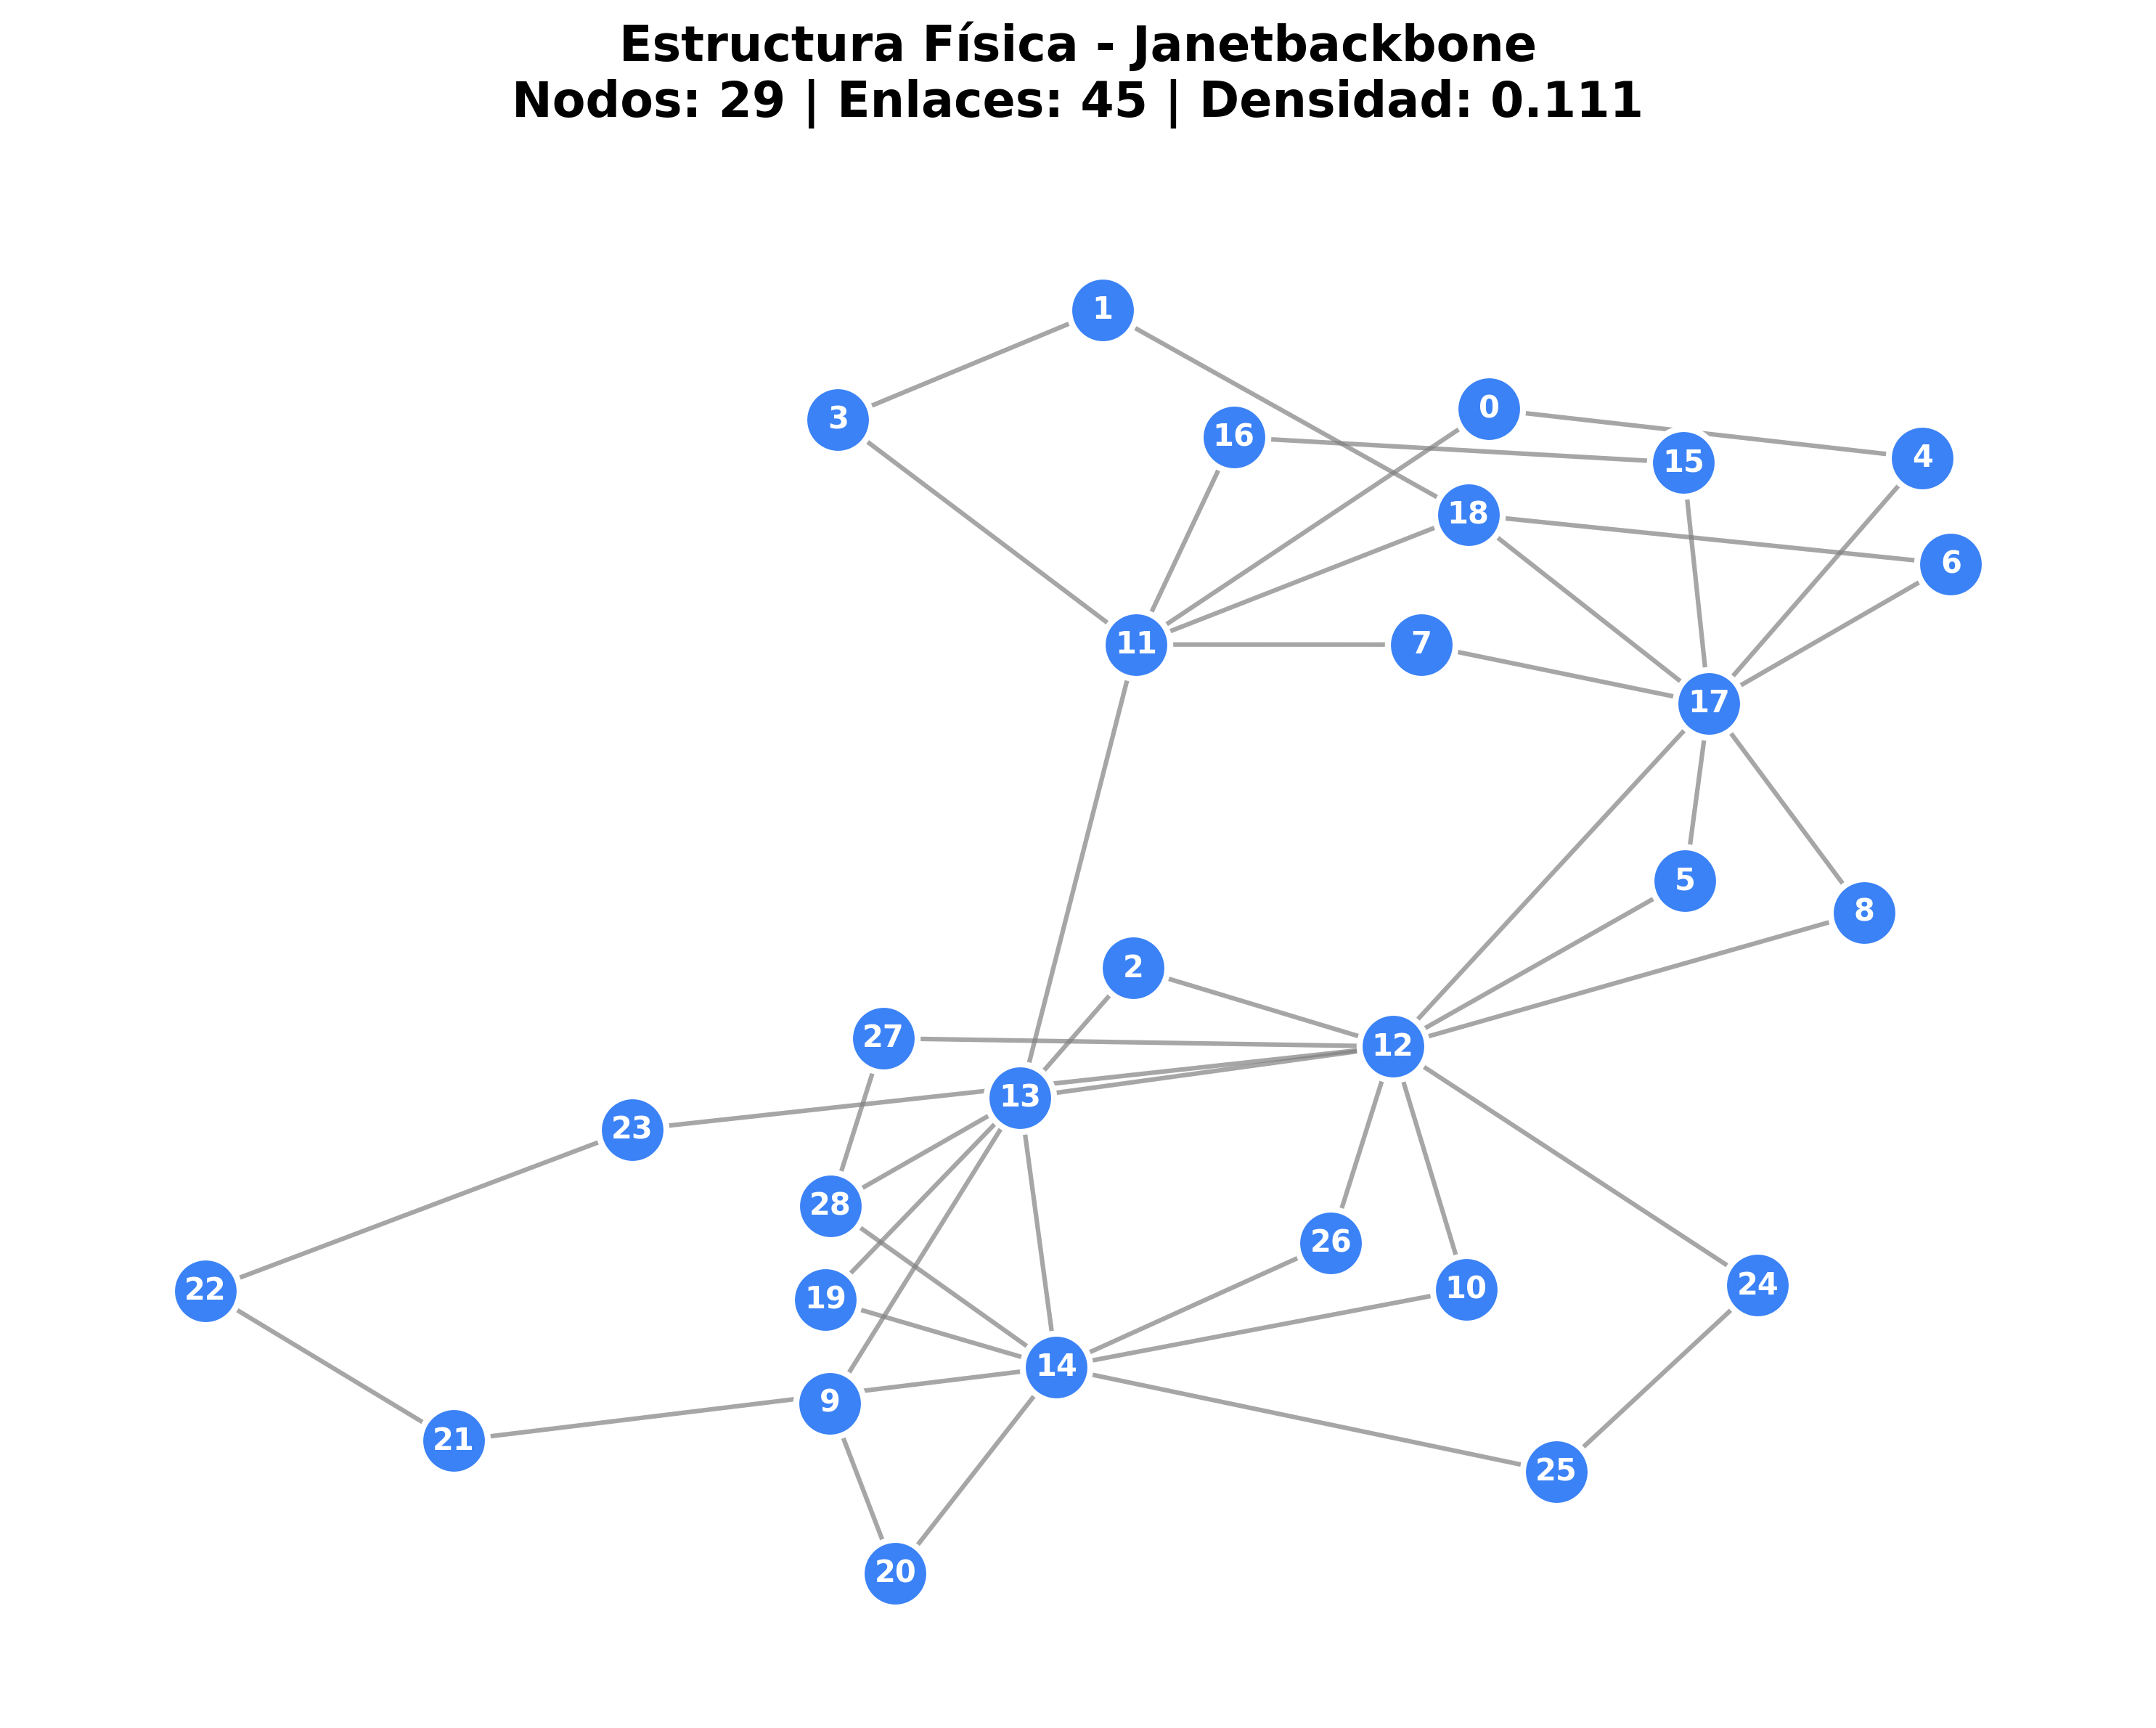
\includegraphics[width=0.5\textwidth]{imagenes/Janetbackbone_estructura.png}\\[2mm]
	{\small (c) Janetbackbone}
	\caption{Estructura de las topologías de evaluación.}
	\label{fig:estructura_redes_evaluacion}
\end{figure}

%
\bibliographystyle{unsrt}
\addcontentsline{toc}{chapter}{Bibliografía}
% \nocite{*} eliminado: solo aparecen en la bibliografía las referencias citadas
\bibliography{bibliografia/bibliografia}
%
%\appendix
%\input{apendices/manual_usuario/manual_usuario}
%%\input{apendices/paper/paper}
%\input{glosario/entradas_glosario}
% \addcontentsline{toc}{chapter}{Glosario}
% \printglossary

\end{document}
